%!TEX root = ../main.tex
% GENERADO por scripts/diccionario/generar.py — no editar a mano.

% 47 tablas, 375 columnas.

\subsection{Esquema \texttt{identidad} (M1)}\label{dd:identidad}

Identidad y perfiles: cuentas de usuario, verificación del tutor (credenciales, especialidades y \gls{cap}), autorizaciones y consentimientos de los menores, y control de reintentos. Tablas: 11. Su diagrama entidad-relación es la figura~\ref{fig:der-identidad}.

\begin{figure}[htbp]
    \centering
    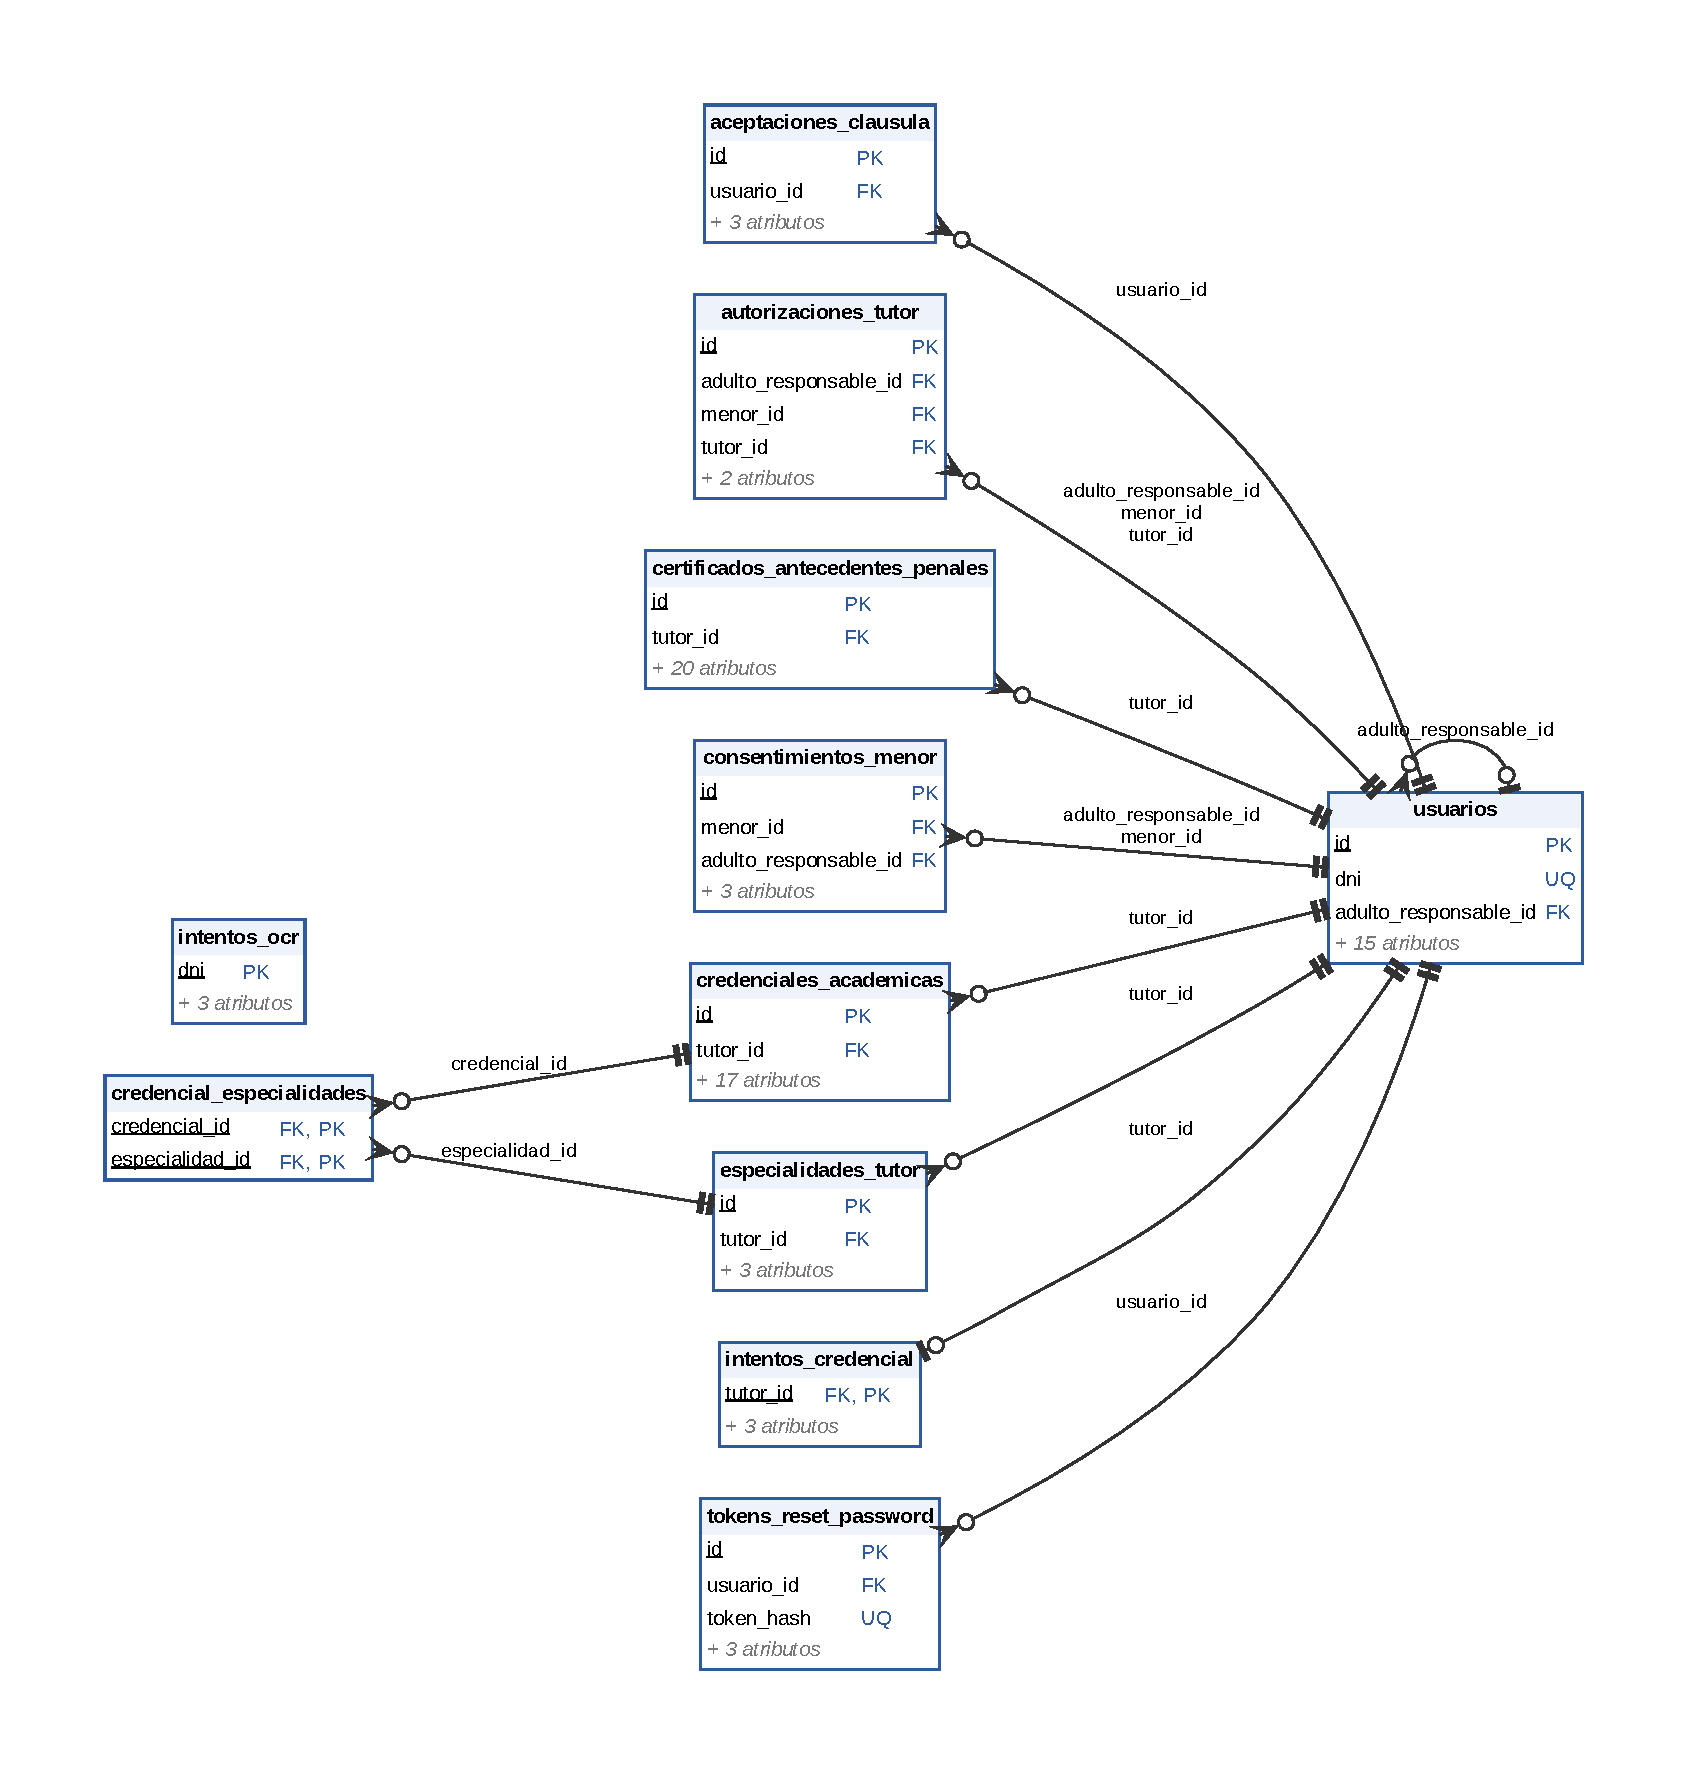
\includegraphics[scale=0.525]{figuras/der/identidad}
    \caption{Diagrama entidad-relación del esquema \texttt{identidad} (M1)}
    \label{fig:der-identidad}
\end{figure}

\subsubsection{\texorpdfstring{\texttt{identidad.aceptaciones\_\allowbreak{}clausula}}{identidad.aceptaciones\_clausula}}\label{dd:identidad.aceptaciones_clausula}

Consentimiento expreso (Ley 25.326): qué usuario aceptó qué versión de qué cláusula (Términos, grabación del audio) y cuándo. \emph{Migraciones:} V36.

{\small
\begin{xltabular}{\textwidth}{@{}>{\raggedright\arraybackslash}p{3.6cm} >{\raggedright\arraybackslash}p{2.3cm} >{\raggedright\arraybackslash}p{1cm} >{\centering\arraybackslash}p{0.85cm} L@{}}
    \toprule
    \tb{Atributo} & \tb{Tipo} & \tb{Clave} & \tb{Nulo} & \tb{Descripción} \\
    \midrule
    \endfirsthead
    \toprule
    \tb{Atributo} & \tb{Tipo} & \tb{Clave} & \tb{Nulo} & \tb{Descripción} \\
    \midrule
    \endhead
    \bottomrule
    \endfoot
    \texttt{id} & \texttt{uuid} & PK & no & Identificador (UUID generado por la base) \\
    \texttt{usuario\_\allowbreak{}id} & \texttt{uuid} & FK & no & Usuario que acepta \\
    \texttt{clausula} & \texttt{varchar(\allowbreak{}50)} &  & no & Cláusula aceptada \\
    \texttt{version} & \texttt{varchar(\allowbreak{}20)} &  & no & Versión del texto aceptado \\
    \texttt{aceptada\_\allowbreak{}at} & \texttt{timestamptz} &  & no & Fecha y hora de la aceptación. Por defecto: \texttt{now(\allowbreak{})} \\
\end{xltabular}
}

{\small
\begin{xltabular}{\textwidth}{@{}>{\raggedright\arraybackslash}p{1.7cm} >{\raggedright\arraybackslash}p{4.6cm} L@{}}
    \toprule
    \tb{Tipo} & \tb{Nombre} & \tb{Definición} \\
    \midrule
    \endfirsthead
    \toprule
    \tb{Tipo} & \tb{Nombre} & \tb{Definición} \\
    \midrule
    \endhead
    \bottomrule
    \endfoot
    FK & \texttt{aceptaciones\_\allowbreak{}clausula\_\allowbreak{}usuario\_\allowbreak{}id\_\allowbreak{}fkey} & \texttt{(\allowbreak{}usuario\_\allowbreak{}id) $\rightarrow$ identidad.usuarios(\allowbreak{}id)} \\
    PK & \texttt{aceptaciones\_\allowbreak{}clausula\_\allowbreak{}pkey} & \texttt{(\allowbreak{}id)} \\
    UNIQUE & \texttt{aceptaciones\_\allowbreak{}clausula\_\allowbreak{}usuario\_\allowbreak{}id\_\allowbreak{}clausula\_\allowbreak{}version\_\allowbreak{}key} & \texttt{(\allowbreak{}usuario\_\allowbreak{}id,\allowbreak{} clausula,\allowbreak{} version)} \\
\end{xltabular}
}

\subsubsection{\texorpdfstring{\texttt{identidad.autorizaciones\_\allowbreak{}tutor}}{identidad.autorizaciones\_tutor}}\label{dd:identidad.autorizaciones_tutor}

Tutores que el Adulto Responsable autorizó para cada uno de sus menores. Un menor solo puede tomar clase con un tutor autorizado. \emph{Migraciones:} V2.

{\small
\begin{xltabular}{\textwidth}{@{}>{\raggedright\arraybackslash}p{3.6cm} >{\raggedright\arraybackslash}p{2.3cm} >{\raggedright\arraybackslash}p{1cm} >{\centering\arraybackslash}p{0.85cm} L@{}}
    \toprule
    \tb{Atributo} & \tb{Tipo} & \tb{Clave} & \tb{Nulo} & \tb{Descripción} \\
    \midrule
    \endfirsthead
    \toprule
    \tb{Atributo} & \tb{Tipo} & \tb{Clave} & \tb{Nulo} & \tb{Descripción} \\
    \midrule
    \endhead
    \bottomrule
    \endfoot
    \texttt{id} & \texttt{uuid} & PK & no & Identificador (UUID generado por la base) \\
    \texttt{adulto\_\allowbreak{}responsable\_\allowbreak{}id} & \texttt{uuid} & FK & no & Adulto Responsable que autoriza \\
    \texttt{menor\_\allowbreak{}id} & \texttt{uuid} & FK & no & Menor al que se aplica la autorización \\
    \texttt{tutor\_\allowbreak{}id} & \texttt{uuid} & FK & no & Tutor autorizado \\
    \texttt{no\_\allowbreak{}confiable} & \texttt{boolean} &  & no & El adulto marcó al tutor como no confiable; bloquea nuevas reservas. Por defecto: \texttt{false} \\
    \texttt{created\_\allowbreak{}at} & \texttt{timestamptz} &  & no & Fecha y hora de la autorización. Por defecto: \texttt{now(\allowbreak{})} \\
\end{xltabular}
}

{\small
\begin{xltabular}{\textwidth}{@{}>{\raggedright\arraybackslash}p{1.7cm} >{\raggedright\arraybackslash}p{4.6cm} L@{}}
    \toprule
    \tb{Tipo} & \tb{Nombre} & \tb{Definición} \\
    \midrule
    \endfirsthead
    \toprule
    \tb{Tipo} & \tb{Nombre} & \tb{Definición} \\
    \midrule
    \endhead
    \bottomrule
    \endfoot
    FK & \texttt{autorizaciones\_\allowbreak{}tutor\_\allowbreak{}adulto\_\allowbreak{}responsable\_\allowbreak{}id\_\allowbreak{}fkey} & \texttt{(\allowbreak{}adulto\_\allowbreak{}responsable\_\allowbreak{}id) $\rightarrow$ identidad.usuarios(\allowbreak{}id)} \\
    FK & \texttt{autorizaciones\_\allowbreak{}tutor\_\allowbreak{}menor\_\allowbreak{}id\_\allowbreak{}fkey} & \texttt{(\allowbreak{}menor\_\allowbreak{}id) $\rightarrow$ identidad.usuarios(\allowbreak{}id)} \\
    FK & \texttt{autorizaciones\_\allowbreak{}tutor\_\allowbreak{}tutor\_\allowbreak{}id\_\allowbreak{}fkey} & \texttt{(\allowbreak{}tutor\_\allowbreak{}id) $\rightarrow$ identidad.usuarios(\allowbreak{}id)} \\
    PK & \texttt{autorizaciones\_\allowbreak{}tutor\_\allowbreak{}pkey} & \texttt{(\allowbreak{}id)} \\
    UNIQUE & \texttt{uq\_\allowbreak{}autorizacion} & \texttt{(\allowbreak{}adulto\_\allowbreak{}responsable\_\allowbreak{}id,\allowbreak{} menor\_\allowbreak{}id,\allowbreak{} tutor\_\allowbreak{}id)} \\
\end{xltabular}
}

\subsubsection{\texorpdfstring{\texttt{identidad.certificados\_\allowbreak{}antecedentes\_\allowbreak{}penales}}{identidad.certificados\_antecedentes\_penales}}\label{dd:identidad.certificados_antecedentes_penales}

\gls{cap} del tutor: habilita a dar clases a menores. Incluye la cola de verificación de la firma digital con el validador oficial (ADR-M1-10). \emph{Migraciones:} V6, V50.

{\small
\begin{xltabular}{\textwidth}{@{}>{\raggedright\arraybackslash}p{3.6cm} >{\raggedright\arraybackslash}p{2.3cm} >{\raggedright\arraybackslash}p{1cm} >{\centering\arraybackslash}p{0.85cm} L@{}}
    \toprule
    \tb{Atributo} & \tb{Tipo} & \tb{Clave} & \tb{Nulo} & \tb{Descripción} \\
    \midrule
    \endfirsthead
    \toprule
    \tb{Atributo} & \tb{Tipo} & \tb{Clave} & \tb{Nulo} & \tb{Descripción} \\
    \midrule
    \endhead
    \bottomrule
    \endfoot
    \texttt{id} & \texttt{uuid} & PK & no & Identificador (UUID generado por la base) \\
    \texttt{tutor\_\allowbreak{}id} & \texttt{uuid} & FK & no & Tutor que presenta el certificado \\
    \texttt{archivo\_\allowbreak{}url} & \texttt{varchar(\allowbreak{}500)} &  & no & Referencia interna del archivo subido \\
    \texttt{fecha\_\allowbreak{}emision} & \texttt{date} &  & no & Fecha de emisión del certificado \\
    \texttt{vence\_\allowbreak{}at} & \texttt{date} &  & no & Fecha de vencimiento \\
    \texttt{estado} & \texttt{varchar(\allowbreak{}20)} &  & no & PENDIENTE, APROBADO, RECHAZADO, EN\_REVISION\_LEGAL (nunca se resuelve sola) o VENCIDO. Por defecto: \texttt{\textquotesingle{}PENDIENTE\textquotesingle{}} \\
    \texttt{tiene\_\allowbreak{}antecedentes} & \texttt{boolean} &  & no & El certificado informa antecedentes. Por defecto: \texttt{false} \\
    \texttt{categoria\_\allowbreak{}antecedente} & \texttt{varchar(\allowbreak{}255)} &  & sí & Categoría del antecedente informado, si lo hay \\
    \texttt{numero\_\allowbreak{}intento} & \texttt{integer} &  & no & Número de intento dentro del ciclo actual (1 a 3). Por defecto: \texttt{1} \\
    \texttt{ciclo\_\allowbreak{}espera\_\allowbreak{}hasta} & \texttt{timestamptz} &  & sí & Fin de la espera tras agotar los intentos del ciclo \\
    \texttt{admin\_\allowbreak{}revisor\_\allowbreak{}id} & \texttt{uuid} &  & sí & Usuario administrador que resolvió la revisión; sin clave foránea declarada \\
    \texttt{created\_\allowbreak{}at} & \texttt{timestamptz} &  & no & Fecha y hora de presentación. Por defecto: \texttt{now(\allowbreak{})} \\
    \texttt{revisado\_\allowbreak{}at} & \texttt{timestamptz} &  & sí & Fecha y hora de la resolución \\
    \texttt{firma\_\allowbreak{}estado} & \texttt{varchar(\allowbreak{}30)} &  & no & Estado de la verificación de la firma digital en la cola. Por defecto: \texttt{\textquotesingle{}NO\_\allowbreak{}VERIFICADA\textquotesingle{}} \\
    \texttt{firma\_\allowbreak{}detalle} & \texttt{varchar(\allowbreak{}500)} &  & sí & Detalle corto del resultado del validador (no se guarda la respuesta completa) \\
    \texttt{firma\_\allowbreak{}firmante} & \texttt{varchar(\allowbreak{}300)} &  & sí & Firmante informado por el validador \\
    \texttt{firma\_\allowbreak{}sha256} & \texttt{varchar(\allowbreak{}64)} &  & sí & Hash del archivo enviado; el resultado solo vale si el validador informa el mismo \\
    \texttt{firma\_\allowbreak{}solicitud\_\allowbreak{}id} & \texttt{varchar(\allowbreak{}120)} &  & sí & Identificador de la solicitud en el validador \\
    \texttt{firma\_\allowbreak{}intentos} & \texttt{integer} &  & no & Intentos de verificación realizados. Por defecto: \texttt{0} \\
    \texttt{firma\_\allowbreak{}proximo\_\allowbreak{}intento\_\allowbreak{}at} & \texttt{timestamptz} &  & sí & Momento del próximo envío o consulta de la cola \\
    \texttt{firma\_\allowbreak{}enviada\_\allowbreak{}at} & \texttt{timestamptz} &  & sí & Fecha y hora del envío al validador \\
    \texttt{firma\_\allowbreak{}verificada\_\allowbreak{}at} & \texttt{timestamptz} &  & sí & Fecha y hora del resultado del validador \\
\end{xltabular}
}

{\small
\begin{xltabular}{\textwidth}{@{}>{\raggedright\arraybackslash}p{1.7cm} >{\raggedright\arraybackslash}p{4.6cm} L@{}}
    \toprule
    \tb{Tipo} & \tb{Nombre} & \tb{Definición} \\
    \midrule
    \endfirsthead
    \toprule
    \tb{Tipo} & \tb{Nombre} & \tb{Definición} \\
    \midrule
    \endhead
    \bottomrule
    \endfoot
    CHECK & \texttt{certificados\_\allowbreak{}antecedentes\_\allowbreak{}penales\_\allowbreak{}estado\_\allowbreak{}check} & \texttt{estado IN (\allowbreak{}\textquotesingle{}PENDIENTE\textquotesingle{},\allowbreak{} \textquotesingle{}APROBADO\textquotesingle{},\allowbreak{} \textquotesingle{}RECHAZADO\textquotesingle{},\allowbreak{} \textquotesingle{}EN\_\allowbreak{}REVISION\_\allowbreak{}LEGAL\textquotesingle{},\allowbreak{} \textquotesingle{}VENCIDO\textquotesingle{})} \\
    CHECK & \texttt{certificados\_\allowbreak{}antecedentes\_\allowbreak{}penales\_\allowbreak{}firma\_\allowbreak{}estado\_\allowbreak{}check} & \texttt{firma\_\allowbreak{}estado IN (\allowbreak{}\textquotesingle{}NO\_\allowbreak{}VERIFICADA\textquotesingle{},\allowbreak{} \textquotesingle{}PENDIENTE\textquotesingle{},\allowbreak{} \textquotesingle{}EN\_\allowbreak{}PROCESO\textquotesingle{},\allowbreak{} \textquotesingle{}VALIDA\textquotesingle{},\allowbreak{} \textquotesingle{}INVALIDA\textquotesingle{},\allowbreak{} \textquotesingle{}FIRMANTE\_\allowbreak{}NO\_\allowbreak{}RECONOCIDO\textquotesingle{},\allowbreak{} \textquotesingle{}ERROR\textquotesingle{})} \\
    CHECK & \texttt{certificados\_\allowbreak{}antecedentes\_\allowbreak{}penales\_\allowbreak{}numero\_\allowbreak{}intento\_\allowbreak{}check} & \texttt{(\allowbreak{}numero\_\allowbreak{}intento \textgreater{}= 1) AND (\allowbreak{}numero\_\allowbreak{}intento \textless{}= 3)} \\
    FK & \texttt{certificados\_\allowbreak{}antecedentes\_\allowbreak{}penales\_\allowbreak{}tutor\_\allowbreak{}id\_\allowbreak{}fkey} & \texttt{(\allowbreak{}tutor\_\allowbreak{}id) $\rightarrow$ identidad.usuarios(\allowbreak{}id)} \\
    PK & \texttt{certificados\_\allowbreak{}antecedentes\_\allowbreak{}penales\_\allowbreak{}pkey} & \texttt{(\allowbreak{}id)} \\
    Índice & \texttt{idx\_\allowbreak{}cap\_\allowbreak{}estado\_\allowbreak{}vence} & \texttt{(\allowbreak{}estado,\allowbreak{} vence\_\allowbreak{}at)} \\
    Índice & \texttt{idx\_\allowbreak{}cap\_\allowbreak{}firma\_\allowbreak{}cola} & \texttt{(\allowbreak{}firma\_\allowbreak{}estado,\allowbreak{} firma\_\allowbreak{}proximo\_\allowbreak{}intento\_\allowbreak{}at)} \\
    Índice & \texttt{idx\_\allowbreak{}cap\_\allowbreak{}tutor} & \texttt{(\allowbreak{}tutor\_\allowbreak{}id)} \\
\end{xltabular}
}

\subsubsection{\texorpdfstring{\texttt{identidad.consentimientos\_\allowbreak{}menor}}{identidad.consentimientos\_menor}}\label{dd:identidad.consentimientos_menor}

Consentimiento del Adulto Responsable para el uso de la plataforma por el menor, con la versión del texto aceptado. \emph{Migraciones:} V2.

{\small
\begin{xltabular}{\textwidth}{@{}>{\raggedright\arraybackslash}p{3.6cm} >{\raggedright\arraybackslash}p{2.3cm} >{\raggedright\arraybackslash}p{1cm} >{\centering\arraybackslash}p{0.85cm} L@{}}
    \toprule
    \tb{Atributo} & \tb{Tipo} & \tb{Clave} & \tb{Nulo} & \tb{Descripción} \\
    \midrule
    \endfirsthead
    \toprule
    \tb{Atributo} & \tb{Tipo} & \tb{Clave} & \tb{Nulo} & \tb{Descripción} \\
    \midrule
    \endhead
    \bottomrule
    \endfoot
    \texttt{id} & \texttt{uuid} & PK & no & Identificador (UUID generado por la base) \\
    \texttt{menor\_\allowbreak{}id} & \texttt{uuid} & FK & no & Menor al que se refiere el consentimiento \\
    \texttt{adulto\_\allowbreak{}responsable\_\allowbreak{}id} & \texttt{uuid} & FK & no & Adulto Responsable que lo otorga \\
    \texttt{version\_\allowbreak{}texto} & \texttt{varchar(\allowbreak{}50)} &  & no & Versión del texto de consentimiento aceptado \\
    \texttt{aceptado\_\allowbreak{}at} & \texttt{timestamptz} &  & no & Fecha y hora de la aceptación. Por defecto: \texttt{now(\allowbreak{})} \\
    \texttt{revocado\_\allowbreak{}at} & \texttt{timestamptz} &  & sí & Fecha y hora de la revocación; nulo si sigue vigente \\
\end{xltabular}
}

{\small
\begin{xltabular}{\textwidth}{@{}>{\raggedright\arraybackslash}p{1.7cm} >{\raggedright\arraybackslash}p{4.6cm} L@{}}
    \toprule
    \tb{Tipo} & \tb{Nombre} & \tb{Definición} \\
    \midrule
    \endfirsthead
    \toprule
    \tb{Tipo} & \tb{Nombre} & \tb{Definición} \\
    \midrule
    \endhead
    \bottomrule
    \endfoot
    FK & \texttt{consentimientos\_\allowbreak{}menor\_\allowbreak{}adulto\_\allowbreak{}responsable\_\allowbreak{}id\_\allowbreak{}fkey} & \texttt{(\allowbreak{}adulto\_\allowbreak{}responsable\_\allowbreak{}id) $\rightarrow$ identidad.usuarios(\allowbreak{}id)} \\
    FK & \texttt{consentimientos\_\allowbreak{}menor\_\allowbreak{}menor\_\allowbreak{}id\_\allowbreak{}fkey} & \texttt{(\allowbreak{}menor\_\allowbreak{}id) $\rightarrow$ identidad.usuarios(\allowbreak{}id)} \\
    PK & \texttt{consentimientos\_\allowbreak{}menor\_\allowbreak{}pkey} & \texttt{(\allowbreak{}id)} \\
    Índice & \texttt{idx\_\allowbreak{}consentimientos\_\allowbreak{}menor} & \texttt{(\allowbreak{}menor\_\allowbreak{}id)} \\
\end{xltabular}
}

\subsubsection{\texorpdfstring{\texttt{identidad.credencial\_\allowbreak{}especialidades}}{identidad.credencial\_especialidades}}\label{dd:identidad.credencial_especialidades}

Tabla asociativa: qué especialidades cubre una credencial aprobada. La elige el administrador al aprobar; si el tutor borra la especialidad, la cobertura se borra con ella. \emph{Migraciones:} V56.

{\small
\begin{xltabular}{\textwidth}{@{}>{\raggedright\arraybackslash}p{3.6cm} >{\raggedright\arraybackslash}p{2.3cm} >{\raggedright\arraybackslash}p{1cm} >{\centering\arraybackslash}p{0.85cm} L@{}}
    \toprule
    \tb{Atributo} & \tb{Tipo} & \tb{Clave} & \tb{Nulo} & \tb{Descripción} \\
    \midrule
    \endfirsthead
    \toprule
    \tb{Atributo} & \tb{Tipo} & \tb{Clave} & \tb{Nulo} & \tb{Descripción} \\
    \midrule
    \endhead
    \bottomrule
    \endfoot
    \texttt{credencial\_\allowbreak{}id} & \texttt{uuid} & FK, PK & no & Credencial aprobada \\
    \texttt{especialidad\_\allowbreak{}id} & \texttt{uuid} & FK, PK & no & Especialidad cubierta \\
\end{xltabular}
}

{\small
\begin{xltabular}{\textwidth}{@{}>{\raggedright\arraybackslash}p{1.7cm} >{\raggedright\arraybackslash}p{4.6cm} L@{}}
    \toprule
    \tb{Tipo} & \tb{Nombre} & \tb{Definición} \\
    \midrule
    \endfirsthead
    \toprule
    \tb{Tipo} & \tb{Nombre} & \tb{Definición} \\
    \midrule
    \endhead
    \bottomrule
    \endfoot
    FK & \texttt{credencial\_\allowbreak{}especialidades\_\allowbreak{}credencial\_\allowbreak{}id\_\allowbreak{}fkey} & \texttt{(\allowbreak{}credencial\_\allowbreak{}id) $\rightarrow$ identidad.credenciales\_\allowbreak{}academicas(\allowbreak{}id)} \\
    FK & \texttt{credencial\_\allowbreak{}especialidades\_\allowbreak{}especialidad\_\allowbreak{}id\_\allowbreak{}fkey} & \texttt{(\allowbreak{}especialidad\_\allowbreak{}id) $\rightarrow$ identidad.especialidades\_\allowbreak{}tutor(\allowbreak{}id)} \texttt{ON DELETE CASCADE} \\
    PK & \texttt{credencial\_\allowbreak{}especialidades\_\allowbreak{}pkey} & \texttt{(\allowbreak{}credencial\_\allowbreak{}id,\allowbreak{} especialidad\_\allowbreak{}id)} \\
    Índice & \texttt{idx\_\allowbreak{}credencial\_\allowbreak{}especialidades\_\allowbreak{}esp} & \texttt{(\allowbreak{}especialidad\_\allowbreak{}id)} \\
\end{xltabular}
}

\subsubsection{\texorpdfstring{\texttt{identidad.credenciales\_\allowbreak{}academicas}}{identidad.credenciales\_academicas}}\label{dd:identidad.credenciales_academicas}

Documento que respalda la formación del tutor, con su triaje automático y la decisión del administrador de moderación. \emph{Migraciones:} V2, V56.

{\small
\begin{xltabular}{\textwidth}{@{}>{\raggedright\arraybackslash}p{3.6cm} >{\raggedright\arraybackslash}p{2.3cm} >{\raggedright\arraybackslash}p{1cm} >{\centering\arraybackslash}p{0.85cm} L@{}}
    \toprule
    \tb{Atributo} & \tb{Tipo} & \tb{Clave} & \tb{Nulo} & \tb{Descripción} \\
    \midrule
    \endfirsthead
    \toprule
    \tb{Atributo} & \tb{Tipo} & \tb{Clave} & \tb{Nulo} & \tb{Descripción} \\
    \midrule
    \endhead
    \bottomrule
    \endfoot
    \texttt{id} & \texttt{uuid} & PK & no & Identificador (UUID generado por la base) \\
    \texttt{tutor\_\allowbreak{}id} & \texttt{uuid} & FK & no & Tutor que presenta la credencial \\
    \texttt{tipo\_\allowbreak{}documento} & \texttt{varchar(\allowbreak{}30)} &  & no & Clase de documento; los tres primeros valores son del esquema anterior a V56 y se siguen admitiendo \\
    \texttt{archivo\_\allowbreak{}url} & \texttt{varchar(\allowbreak{}500)} &  & no & Referencia interna del archivo subido \\
    \texttt{estado} & \texttt{varchar(\allowbreak{}20)} &  & no & PENDIENTE, APROBADO o RECHAZADO. Por defecto: \texttt{\textquotesingle{}PENDIENTE\textquotesingle{}} \\
    \texttt{numero\_\allowbreak{}intento} & \texttt{integer} &  & no & Número de intento dentro del ciclo actual (1 a 3). Por defecto: \texttt{1} \\
    \texttt{ciclo\_\allowbreak{}espera\_\allowbreak{}hasta} & \texttt{timestamptz} &  & sí & Fin de la espera tras agotar los intentos del ciclo \\
    \texttt{admin\_\allowbreak{}revisor\_\allowbreak{}id} & \texttt{uuid} &  & sí & Usuario administrador que resolvió la revisión; sin clave foránea declarada \\
    \texttt{created\_\allowbreak{}at} & \texttt{timestamptz} &  & no & Fecha y hora de presentación. Por defecto: \texttt{now(\allowbreak{})} \\
    \texttt{revisado\_\allowbreak{}at} & \texttt{timestamptz} &  & sí & Fecha y hora de la resolución \\
    \texttt{institucion} & \texttt{varchar(\allowbreak{}200)} &  & sí & Institución que emitió el título \\
    \texttt{denominacion} & \texttt{varchar(\allowbreak{}200)} &  & sí & Nombre del título o de la carrera \\
    \texttt{anio\_\allowbreak{}egreso} & \texttt{integer} &  & sí & Año de egreso (1900 a 2100) \\
    \texttt{es\_\allowbreak{}digital} & \texttt{boolean} &  & sí & El documento es un título digital con enlace de verificación \\
    \texttt{enlace\_\allowbreak{}verificacion} & \texttt{varchar(\allowbreak{}500)} &  & sí & Enlace de verificación del título digital \\
    \texttt{nombre\_\allowbreak{}coincide} & \texttt{boolean} &  & sí & Resultado del \gls{ocr} contra el nombre del \gls{dni}; nulo si no se pudo comparar. Solo marca, nunca rechaza \\
    \texttt{metodo\_\allowbreak{}verificacion} & \texttt{varchar(\allowbreak{}20)} &  & sí & Cómo se aprobó: contra el registro oficial o solo con el documento \\
    \texttt{motivo\_\allowbreak{}rechazo} & \texttt{varchar(\allowbreak{}30)} &  & sí & Motivo codificado del rechazo \\
    \texttt{detalle\_\allowbreak{}rechazo} & \texttt{varchar(\allowbreak{}500)} &  & sí & Explicación libre del rechazo para el tutor \\
\end{xltabular}
}

{\small
\begin{xltabular}{\textwidth}{@{}>{\raggedright\arraybackslash}p{1.7cm} >{\raggedright\arraybackslash}p{4.6cm} L@{}}
    \toprule
    \tb{Tipo} & \tb{Nombre} & \tb{Definición} \\
    \midrule
    \endfirsthead
    \toprule
    \tb{Tipo} & \tb{Nombre} & \tb{Definición} \\
    \midrule
    \endhead
    \bottomrule
    \endfoot
    CHECK & \texttt{credenciales\_\allowbreak{}academicas\_\allowbreak{}anio\_\allowbreak{}egreso\_\allowbreak{}check} & \texttt{(\allowbreak{}anio\_\allowbreak{}egreso \textgreater{}= 1900) AND (\allowbreak{}anio\_\allowbreak{}egreso \textless{}= 2100)} \\
    CHECK & \texttt{credenciales\_\allowbreak{}academicas\_\allowbreak{}estado\_\allowbreak{}check} & \texttt{estado IN (\allowbreak{}\textquotesingle{}PENDIENTE\textquotesingle{},\allowbreak{} \textquotesingle{}APROBADO\textquotesingle{},\allowbreak{} \textquotesingle{}RECHAZADO\textquotesingle{})} \\
    CHECK & \texttt{credenciales\_\allowbreak{}academicas\_\allowbreak{}metodo\_\allowbreak{}verificacion\_\allowbreak{}check} & \texttt{metodo\_\allowbreak{}verificacion IN (\allowbreak{}\textquotesingle{}REGISTRO\_\allowbreak{}OFICIAL\textquotesingle{},\allowbreak{} \textquotesingle{}SOLO\_\allowbreak{}DOCUMENTO\textquotesingle{})} \\
    CHECK & \texttt{credenciales\_\allowbreak{}academicas\_\allowbreak{}motivo\_\allowbreak{}rechazo\_\allowbreak{}check} & \texttt{motivo\_\allowbreak{}rechazo IN (\allowbreak{}\textquotesingle{}ILEGIBLE\textquotesingle{},\allowbreak{} \textquotesingle{}NO\_\allowbreak{}ES\_\allowbreak{}TITULO\textquotesingle{},\allowbreak{} \textquotesingle{}NOMBRE\_\allowbreak{}NO\_\allowbreak{}COINCIDE\textquotesingle{},\allowbreak{} \textquotesingle{}NO\_\allowbreak{}FIGURA\_\allowbreak{}EN\_\allowbreak{}REGISTRO\textquotesingle{},\allowbreak{} \textquotesingle{}DATOS\_\allowbreak{}NO\_\allowbreak{}COINCIDEN\textquotesingle{},\allowbreak{} \textquotesingle{}ENLACE\_\allowbreak{}INVALIDO\textquotesingle{},\allowbreak{} \textquotesingle{}OTRO\textquotesingle{})} \\
    CHECK & \texttt{credenciales\_\allowbreak{}academicas\_\allowbreak{}numero\_\allowbreak{}intento\_\allowbreak{}check} & \texttt{(\allowbreak{}numero\_\allowbreak{}intento \textgreater{}= 1) AND (\allowbreak{}numero\_\allowbreak{}intento \textless{}= 3)} \\
    CHECK & \texttt{credenciales\_\allowbreak{}academicas\_\allowbreak{}tipo\_\allowbreak{}documento\_\allowbreak{}check} & \texttt{tipo\_\allowbreak{}documento IN (\allowbreak{}\textquotesingle{}TITULO\textquotesingle{},\allowbreak{} \textquotesingle{}CERTIFICADO\_\allowbreak{}ANALITICO\textquotesingle{},\allowbreak{} \textquotesingle{}MATRICULA\textquotesingle{},\allowbreak{} \textquotesingle{}SECUNDARIO\textquotesingle{},\allowbreak{} \textquotesingle{}TERCIARIO\_\allowbreak{}NO\_\allowbreak{}DOCENTE\textquotesingle{},\allowbreak{} \textquotesingle{}PROFESORADO\textquotesingle{},\allowbreak{} \textquotesingle{}UNIVERSITARIO\textquotesingle{},\allowbreak{} \textquotesingle{}ALUMNO\_\allowbreak{}UNIVERSITARIO\textquotesingle{},\allowbreak{} \textquotesingle{}MATRICULA\_\allowbreak{}PROFESIONAL\textquotesingle{},\allowbreak{} \textquotesingle{}OTRO\textquotesingle{})} \\
    FK & \texttt{credenciales\_\allowbreak{}academicas\_\allowbreak{}tutor\_\allowbreak{}id\_\allowbreak{}fkey} & \texttt{(\allowbreak{}tutor\_\allowbreak{}id) $\rightarrow$ identidad.usuarios(\allowbreak{}id)} \\
    PK & \texttt{credenciales\_\allowbreak{}academicas\_\allowbreak{}pkey} & \texttt{(\allowbreak{}id)} \\
    Índice & \texttt{idx\_\allowbreak{}credenciales\_\allowbreak{}estado} & \texttt{(\allowbreak{}estado)} \\
    Índice & \texttt{idx\_\allowbreak{}credenciales\_\allowbreak{}tutor} & \texttt{(\allowbreak{}tutor\_\allowbreak{}id)} \\
\end{xltabular}
}

\subsubsection{\texorpdfstring{\texttt{identidad.especialidades\_\allowbreak{}tutor}}{identidad.especialidades\_tutor}}\label{dd:identidad.especialidades_tutor}

Materias que el tutor declara enseñar (de una a tres) con el nivel máximo. Su estado de verificación no se guarda: se deriva de las credenciales aprobadas que la cubren. Se usa solo con \path{tinku.especialidades.habilitado}. \emph{Migraciones:} V56.

{\small
\begin{xltabular}{\textwidth}{@{}>{\raggedright\arraybackslash}p{3.6cm} >{\raggedright\arraybackslash}p{2.3cm} >{\raggedright\arraybackslash}p{1cm} >{\centering\arraybackslash}p{0.85cm} L@{}}
    \toprule
    \tb{Atributo} & \tb{Tipo} & \tb{Clave} & \tb{Nulo} & \tb{Descripción} \\
    \midrule
    \endfirsthead
    \toprule
    \tb{Atributo} & \tb{Tipo} & \tb{Clave} & \tb{Nulo} & \tb{Descripción} \\
    \midrule
    \endhead
    \bottomrule
    \endfoot
    \texttt{id} & \texttt{uuid} & PK & no & Identificador (UUID generado por la base) \\
    \texttt{tutor\_\allowbreak{}id} & \texttt{uuid} & FK & no & Tutor que declara la especialidad \\
    \texttt{materia} & \texttt{varchar(\allowbreak{}100)} &  & no & Materia del catálogo de temas \\
    \texttt{nivel\_\allowbreak{}maximo} & \texttt{varchar(\allowbreak{}20)} &  & no & Nivel más alto que puede enseñar: PRIMARIO, SECUNDARIO o UNIVERSITARIO \\
    \texttt{created\_\allowbreak{}at} & \texttt{timestamptz} &  & no & Fecha y hora de creación de la fila. Por defecto: \texttt{now(\allowbreak{})} \\
\end{xltabular}
}

{\small
\begin{xltabular}{\textwidth}{@{}>{\raggedright\arraybackslash}p{1.7cm} >{\raggedright\arraybackslash}p{4.6cm} L@{}}
    \toprule
    \tb{Tipo} & \tb{Nombre} & \tb{Definición} \\
    \midrule
    \endfirsthead
    \toprule
    \tb{Tipo} & \tb{Nombre} & \tb{Definición} \\
    \midrule
    \endhead
    \bottomrule
    \endfoot
    CHECK & \texttt{especialidades\_\allowbreak{}tutor\_\allowbreak{}nivel\_\allowbreak{}maximo\_\allowbreak{}check} & \texttt{nivel\_\allowbreak{}maximo IN (\allowbreak{}\textquotesingle{}PRIMARIO\textquotesingle{},\allowbreak{} \textquotesingle{}SECUNDARIO\textquotesingle{},\allowbreak{} \textquotesingle{}UNIVERSITARIO\textquotesingle{})} \\
    FK & \texttt{especialidades\_\allowbreak{}tutor\_\allowbreak{}tutor\_\allowbreak{}id\_\allowbreak{}fkey} & \texttt{(\allowbreak{}tutor\_\allowbreak{}id) $\rightarrow$ identidad.usuarios(\allowbreak{}id)} \\
    PK & \texttt{especialidades\_\allowbreak{}tutor\_\allowbreak{}pkey} & \texttt{(\allowbreak{}id)} \\
    UNIQUE & \texttt{uq\_\allowbreak{}especialidad\_\allowbreak{}tutor\_\allowbreak{}materia} & \texttt{(\allowbreak{}tutor\_\allowbreak{}id,\allowbreak{} materia)} \\
    Índice & \texttt{idx\_\allowbreak{}especialidades\_\allowbreak{}tutor} & \texttt{(\allowbreak{}tutor\_\allowbreak{}id)} \\
\end{xltabular}
}

\subsubsection{\texorpdfstring{\texttt{identidad.intentos\_\allowbreak{}credencial}}{identidad.intentos\_credencial}}\label{dd:identidad.intentos_credencial}

Ciclos de reintento de credencial agotados por cada tutor, para escalar la espera (24, 48, 96 horas\ldots). La comparten credenciales y \gls{cap}. \emph{Migraciones:} V5.

{\small
\begin{xltabular}{\textwidth}{@{}>{\raggedright\arraybackslash}p{3.6cm} >{\raggedright\arraybackslash}p{2.3cm} >{\raggedright\arraybackslash}p{1cm} >{\centering\arraybackslash}p{0.85cm} L@{}}
    \toprule
    \tb{Atributo} & \tb{Tipo} & \tb{Clave} & \tb{Nulo} & \tb{Descripción} \\
    \midrule
    \endfirsthead
    \toprule
    \tb{Atributo} & \tb{Tipo} & \tb{Clave} & \tb{Nulo} & \tb{Descripción} \\
    \midrule
    \endhead
    \bottomrule
    \endfoot
    \texttt{tutor\_\allowbreak{}id} & \texttt{uuid} & FK, PK & no & Tutor al que corresponde el contador \\
    \texttt{veces\_\allowbreak{}ciclo\_\allowbreak{}agotado} & \texttt{integer} &  & no & Cantidad de ciclos agotados; la espera es $24 \cdot 2^n$ horas. Por defecto: \texttt{0} \\
    \texttt{proximo\_\allowbreak{}intento\_\allowbreak{}permitido} & \texttt{timestamptz} &  & sí & Fin de la espera actual; nulo si no hay espera \\
    \texttt{updated\_\allowbreak{}at} & \texttt{timestamptz} &  & no & Fecha y hora de la última modificación. Por defecto: \texttt{now(\allowbreak{})} \\
\end{xltabular}
}

{\small
\begin{xltabular}{\textwidth}{@{}>{\raggedright\arraybackslash}p{1.7cm} >{\raggedright\arraybackslash}p{4.6cm} L@{}}
    \toprule
    \tb{Tipo} & \tb{Nombre} & \tb{Definición} \\
    \midrule
    \endfirsthead
    \toprule
    \tb{Tipo} & \tb{Nombre} & \tb{Definición} \\
    \midrule
    \endhead
    \bottomrule
    \endfoot
    FK & \texttt{intentos\_\allowbreak{}credencial\_\allowbreak{}tutor\_\allowbreak{}id\_\allowbreak{}fkey} & \texttt{(\allowbreak{}tutor\_\allowbreak{}id) $\rightarrow$ identidad.usuarios(\allowbreak{}id)} \\
    PK & \texttt{intentos\_\allowbreak{}credencial\_\allowbreak{}pkey} & \texttt{(\allowbreak{}tutor\_\allowbreak{}id)} \\
\end{xltabular}
}

\subsubsection{\texorpdfstring{\texttt{identidad.intentos\_\allowbreak{}ocr}}{identidad.intentos\_ocr}}\label{dd:identidad.intentos_ocr}

Reintentos de la foto del \gls{dni} en el alta, por \gls{dni} declarado. La espera se evalúa al leer, sin trabajo programado. \emph{Migraciones:} V4, V52.

{\small
\begin{xltabular}{\textwidth}{@{}>{\raggedright\arraybackslash}p{3.6cm} >{\raggedright\arraybackslash}p{2.3cm} >{\raggedright\arraybackslash}p{1cm} >{\centering\arraybackslash}p{0.85cm} L@{}}
    \toprule
    \tb{Atributo} & \tb{Tipo} & \tb{Clave} & \tb{Nulo} & \tb{Descripción} \\
    \midrule
    \endfirsthead
    \toprule
    \tb{Atributo} & \tb{Tipo} & \tb{Clave} & \tb{Nulo} & \tb{Descripción} \\
    \midrule
    \endhead
    \bottomrule
    \endfoot
    \texttt{dni} & \texttt{varchar(\allowbreak{}20)} & PK & no & \gls{dni} declarado por quien intenta registrarse \\
    \texttt{intentos\_\allowbreak{}consumidos} & \texttt{integer} &  & no & Fotos ilegibles en el ciclo actual; el tope lo fija la aplicación (\path{tinku.ocr.max-intentos}). Por defecto: \texttt{0} \\
    \texttt{proximo\_\allowbreak{}intento\_\allowbreak{}permitido} & \texttt{timestamptz} &  & sí & Fin de la espera de 24 horas; nulo si no hay espera \\
    \texttt{updated\_\allowbreak{}at} & \texttt{timestamptz} &  & no & Fecha y hora de la última modificación. Por defecto: \texttt{now(\allowbreak{})} \\
\end{xltabular}
}

{\small
\begin{xltabular}{\textwidth}{@{}>{\raggedright\arraybackslash}p{1.7cm} >{\raggedright\arraybackslash}p{4.6cm} L@{}}
    \toprule
    \tb{Tipo} & \tb{Nombre} & \tb{Definición} \\
    \midrule
    \endfirsthead
    \toprule
    \tb{Tipo} & \tb{Nombre} & \tb{Definición} \\
    \midrule
    \endhead
    \bottomrule
    \endfoot
    CHECK & \texttt{intentos\_\allowbreak{}ocr\_\allowbreak{}intentos\_\allowbreak{}consumidos\_\allowbreak{}check} & \texttt{intentos\_\allowbreak{}consumidos \textgreater{}= 0} \\
    PK & \texttt{intentos\_\allowbreak{}ocr\_\allowbreak{}pkey} & \texttt{(\allowbreak{}dni)} \\
\end{xltabular}
}

\subsubsection{\texorpdfstring{\texttt{identidad.tokens\_\allowbreak{}reset\_\allowbreak{}password}}{identidad.tokens\_reset\_password}}\label{dd:identidad.tokens_reset_password}

Recuperación de contraseña: token opaco de un solo uso. Se guarda solo su hash, de modo que una filtración de la tabla no permite restablecer cuentas. \emph{Migraciones:} V23.

{\small
\begin{xltabular}{\textwidth}{@{}>{\raggedright\arraybackslash}p{3.6cm} >{\raggedright\arraybackslash}p{2.3cm} >{\raggedright\arraybackslash}p{1cm} >{\centering\arraybackslash}p{0.85cm} L@{}}
    \toprule
    \tb{Atributo} & \tb{Tipo} & \tb{Clave} & \tb{Nulo} & \tb{Descripción} \\
    \midrule
    \endfirsthead
    \toprule
    \tb{Atributo} & \tb{Tipo} & \tb{Clave} & \tb{Nulo} & \tb{Descripción} \\
    \midrule
    \endhead
    \bottomrule
    \endfoot
    \texttt{id} & \texttt{uuid} & PK & no & Identificador (UUID generado por la aplicación) \\
    \texttt{usuario\_\allowbreak{}id} & \texttt{uuid} & FK & no & Usuario que pidió el restablecimiento \\
    \texttt{token\_\allowbreak{}hash} & \texttt{varchar(\allowbreak{}64)} & UQ & no & Hash SHA-256 (64 caracteres hexadecimales) del token enviado por correo \\
    \texttt{expira\_\allowbreak{}en} & \texttt{timestamptz} &  & no & Vencimiento del token \\
    \texttt{usado\_\allowbreak{}en} & \texttt{timestamptz} &  & sí & Fecha y hora de uso; nulo si no se usó \\
    \texttt{created\_\allowbreak{}at} & \texttt{timestamptz} &  & no & Fecha y hora de creación de la fila. Por defecto: \texttt{now(\allowbreak{})} \\
\end{xltabular}
}

{\small
\begin{xltabular}{\textwidth}{@{}>{\raggedright\arraybackslash}p{1.7cm} >{\raggedright\arraybackslash}p{4.6cm} L@{}}
    \toprule
    \tb{Tipo} & \tb{Nombre} & \tb{Definición} \\
    \midrule
    \endfirsthead
    \toprule
    \tb{Tipo} & \tb{Nombre} & \tb{Definición} \\
    \midrule
    \endhead
    \bottomrule
    \endfoot
    FK & \texttt{tokens\_\allowbreak{}reset\_\allowbreak{}password\_\allowbreak{}usuario\_\allowbreak{}id\_\allowbreak{}fkey} & \texttt{(\allowbreak{}usuario\_\allowbreak{}id) $\rightarrow$ identidad.usuarios(\allowbreak{}id)} \\
    PK & \texttt{tokens\_\allowbreak{}reset\_\allowbreak{}password\_\allowbreak{}pkey} & \texttt{(\allowbreak{}id)} \\
    UNIQUE & \texttt{tokens\_\allowbreak{}reset\_\allowbreak{}password\_\allowbreak{}token\_\allowbreak{}hash\_\allowbreak{}key} & \texttt{(\allowbreak{}token\_\allowbreak{}hash)} \\
    Índice & \texttt{ix\_\allowbreak{}tokens\_\allowbreak{}reset\_\allowbreak{}password\_\allowbreak{}usuario} & \texttt{(\allowbreak{}usuario\_\allowbreak{}id)} \\
\end{xltabular}
}

\subsubsection{\texorpdfstring{\texttt{identidad.usuarios}}{identidad.usuarios}}\label{dd:identidad.usuarios}

Cuenta de cada persona registrada. Un adulto tiene al menos una de dos capacidades (estudiante y Adulto Responsable); un menor siempre está vinculado a su Adulto Responsable. Los administradores también son usuarios (ver \path{admin.admins}). \emph{Migraciones:} V2, V5, V6, V7, V8, V9, V12, V13, V14, V16, V17, V18, V22, V23, V27, V28, V32, V33, V36, V39, V41, V46, V56, V58.

{\small
\begin{xltabular}{\textwidth}{@{}>{\raggedright\arraybackslash}p{3.6cm} >{\raggedright\arraybackslash}p{2.3cm} >{\raggedright\arraybackslash}p{1cm} >{\centering\arraybackslash}p{0.85cm} L@{}}
    \toprule
    \tb{Atributo} & \tb{Tipo} & \tb{Clave} & \tb{Nulo} & \tb{Descripción} \\
    \midrule
    \endfirsthead
    \toprule
    \tb{Atributo} & \tb{Tipo} & \tb{Clave} & \tb{Nulo} & \tb{Descripción} \\
    \midrule
    \endhead
    \bottomrule
    \endfoot
    \texttt{id} & \texttt{uuid} & PK & no & Identificador (UUID generado por la base) \\
    \texttt{dni} & \texttt{varchar(\allowbreak{}20)} & UQ & no & \gls{dni} verificado por \gls{ocr} al registrarse; es el identificador de inicio de sesión \\
    \texttt{nombre} & \texttt{varchar(\allowbreak{}150)} &  & no & Nombre, tal como figura en el \gls{dni} \\
    \texttt{apellido} & \texttt{varchar(\allowbreak{}150)} &  & no & Apellido, tal como figura en el \gls{dni} \\
    \texttt{fecha\_\allowbreak{}nacimiento} & \texttt{date} &  & no & Fecha de nacimiento; define si la cuenta es de un menor \\
    \texttt{tipo} & \texttt{varchar(\allowbreak{}20)} &  & no & Tipo de cuenta: ADULTO, MENOR o TUTOR \\
    \texttt{capacidad\_\allowbreak{}estudiante} & \texttt{boolean} &  & no & El adulto toma clases para sí mismo. Por defecto: \texttt{false} \\
    \texttt{capacidad\_\allowbreak{}adulto\_\allowbreak{}responsable} & \texttt{boolean} &  & no & El adulto tiene menores a cargo. Por defecto: \texttt{false} \\
    \texttt{adulto\_\allowbreak{}responsable\_\allowbreak{}id} & \texttt{uuid} & FK & sí & Adulto Responsable del menor; obligatorio solo para el tipo MENOR \\
    \texttt{password\_\allowbreak{}hash} & \texttt{varchar(\allowbreak{}255)} &  & no & Hash de la contraseña (nunca la contraseña) \\
    \texttt{estado\_\allowbreak{}cuenta} & \texttt{varchar(\allowbreak{}20)} &  & no & ACTIVA, SUSPENDIDA o BAJA; una baja anonimiza los datos en lugar de borrar la fila (ADR-M1-05). Por defecto: \texttt{\textquotesingle{}ACTIVA\textquotesingle{}} \\
    \texttt{created\_\allowbreak{}at} & \texttt{timestamptz} &  & no & Fecha y hora del alta. Por defecto: \texttt{now(\allowbreak{})} \\
    \texttt{activo\_\allowbreak{}para\_\allowbreak{}matching} & \texttt{boolean} &  & no & El tutor puede aparecer en las búsquedas; lo apagan el vencimiento del \gls{cap} y las sanciones. Por defecto: \texttt{false} \\
    \texttt{email} & \texttt{varchar(\allowbreak{}255)} &  & sí & Correo de contacto; único entre los no nulos. Es nulo en cuentas anteriores a V18 \\
    \texttt{bio} & \texttt{varchar(\allowbreak{}500)} &  & sí & Presentación del tutor en su perfil público (hasta 500 caracteres) \\
    \texttt{foto\_\allowbreak{}ref} & \texttt{text} &  & sí & Referencia interna de la foto de perfil en el almacenamiento (nunca una URL pública) \\
    \texttt{credentials\_\allowbreak{}version} & \texttt{integer} &  & no & Versión de las credenciales; cambia con la contraseña e invalida los \gls{jwt} emitidos antes. Por defecto: \texttt{0} \\
    \texttt{acepta\_\allowbreak{}menores} & \texttt{boolean} &  & no & Preferencia del tutor de dar clases a menores; con \texttt{false} no aparece para ningún menor. Por defecto: \texttt{true} \\
\end{xltabular}
}

{\small
\begin{xltabular}{\textwidth}{@{}>{\raggedright\arraybackslash}p{1.7cm} >{\raggedright\arraybackslash}p{4.6cm} L@{}}
    \toprule
    \tb{Tipo} & \tb{Nombre} & \tb{Definición} \\
    \midrule
    \endfirsthead
    \toprule
    \tb{Tipo} & \tb{Nombre} & \tb{Definición} \\
    \midrule
    \endhead
    \bottomrule
    \endfoot
    CHECK & \texttt{chk\_\allowbreak{}adulto\_\allowbreak{}tiene\_\allowbreak{}capacidad} & \texttt{(\allowbreak{}tipo \textless{}\textgreater{} \textquotesingle{}ADULTO\textquotesingle{}) OR (\allowbreak{}capacidad\_\allowbreak{}estudiante OR capacidad\_\allowbreak{}adulto\_\allowbreak{}responsable)} \\
    CHECK & \texttt{chk\_\allowbreak{}menor\_\allowbreak{}tiene\_\allowbreak{}responsable} & \texttt{(\allowbreak{}(\allowbreak{}tipo = \textquotesingle{}MENOR\textquotesingle{}) AND (\allowbreak{}adulto\_\allowbreak{}responsable\_\allowbreak{}id IS NOT NULL)) OR (\allowbreak{}(\allowbreak{}tipo \textless{}\textgreater{} \textquotesingle{}MENOR\textquotesingle{}) AND (\allowbreak{}adulto\_\allowbreak{}responsable\_\allowbreak{}id IS NULL))} \\
    CHECK & \texttt{chk\_\allowbreak{}usuarios\_\allowbreak{}estado\_\allowbreak{}cuenta} & \texttt{estado\_\allowbreak{}cuenta IN (\allowbreak{}\textquotesingle{}ACTIVA\textquotesingle{},\allowbreak{} \textquotesingle{}SUSPENDIDA\textquotesingle{},\allowbreak{} \textquotesingle{}BAJA\textquotesingle{})} \\
    CHECK & \texttt{usuarios\_\allowbreak{}tipo\_\allowbreak{}check} & \texttt{tipo IN (\allowbreak{}\textquotesingle{}ADULTO\textquotesingle{},\allowbreak{} \textquotesingle{}MENOR\textquotesingle{},\allowbreak{} \textquotesingle{}TUTOR\textquotesingle{})} \\
    FK & \texttt{usuarios\_\allowbreak{}adulto\_\allowbreak{}responsable\_\allowbreak{}id\_\allowbreak{}fkey} & \texttt{(\allowbreak{}adulto\_\allowbreak{}responsable\_\allowbreak{}id) $\rightarrow$ identidad.usuarios(\allowbreak{}id)} \\
    PK & \texttt{usuarios\_\allowbreak{}pkey} & \texttt{(\allowbreak{}id)} \\
    UNIQUE & \texttt{usuarios\_\allowbreak{}dni\_\allowbreak{}key} & \texttt{(\allowbreak{}dni)} \\
    Índice & \texttt{idx\_\allowbreak{}usuarios\_\allowbreak{}adulto\_\allowbreak{}responsable} & \texttt{(\allowbreak{}adulto\_\allowbreak{}responsable\_\allowbreak{}id)} \\
    Índice & \texttt{idx\_\allowbreak{}usuarios\_\allowbreak{}tipo} & \texttt{(\allowbreak{}tipo)} \\
    UNIQUE & \texttt{uq\_\allowbreak{}usuarios\_\allowbreak{}email} & \texttt{(\allowbreak{}email) WHERE email IS NOT NULL} \\
\end{xltabular}
}

\subsection{Esquema \texttt{matching} (M2)}\label{dd:matching}

Motor de \gls{matching}: catálogo de trayectos y temas con sus \gls{embeddings}, perfil semántico del tutor, búsquedas guardadas, temas buscados sin cobertura e instrumentación de la evaluación. Tablas: 8. Su diagrama entidad-relación es la figura~\ref{fig:der-matching}.

\begin{figure}[htbp]
    \centering
    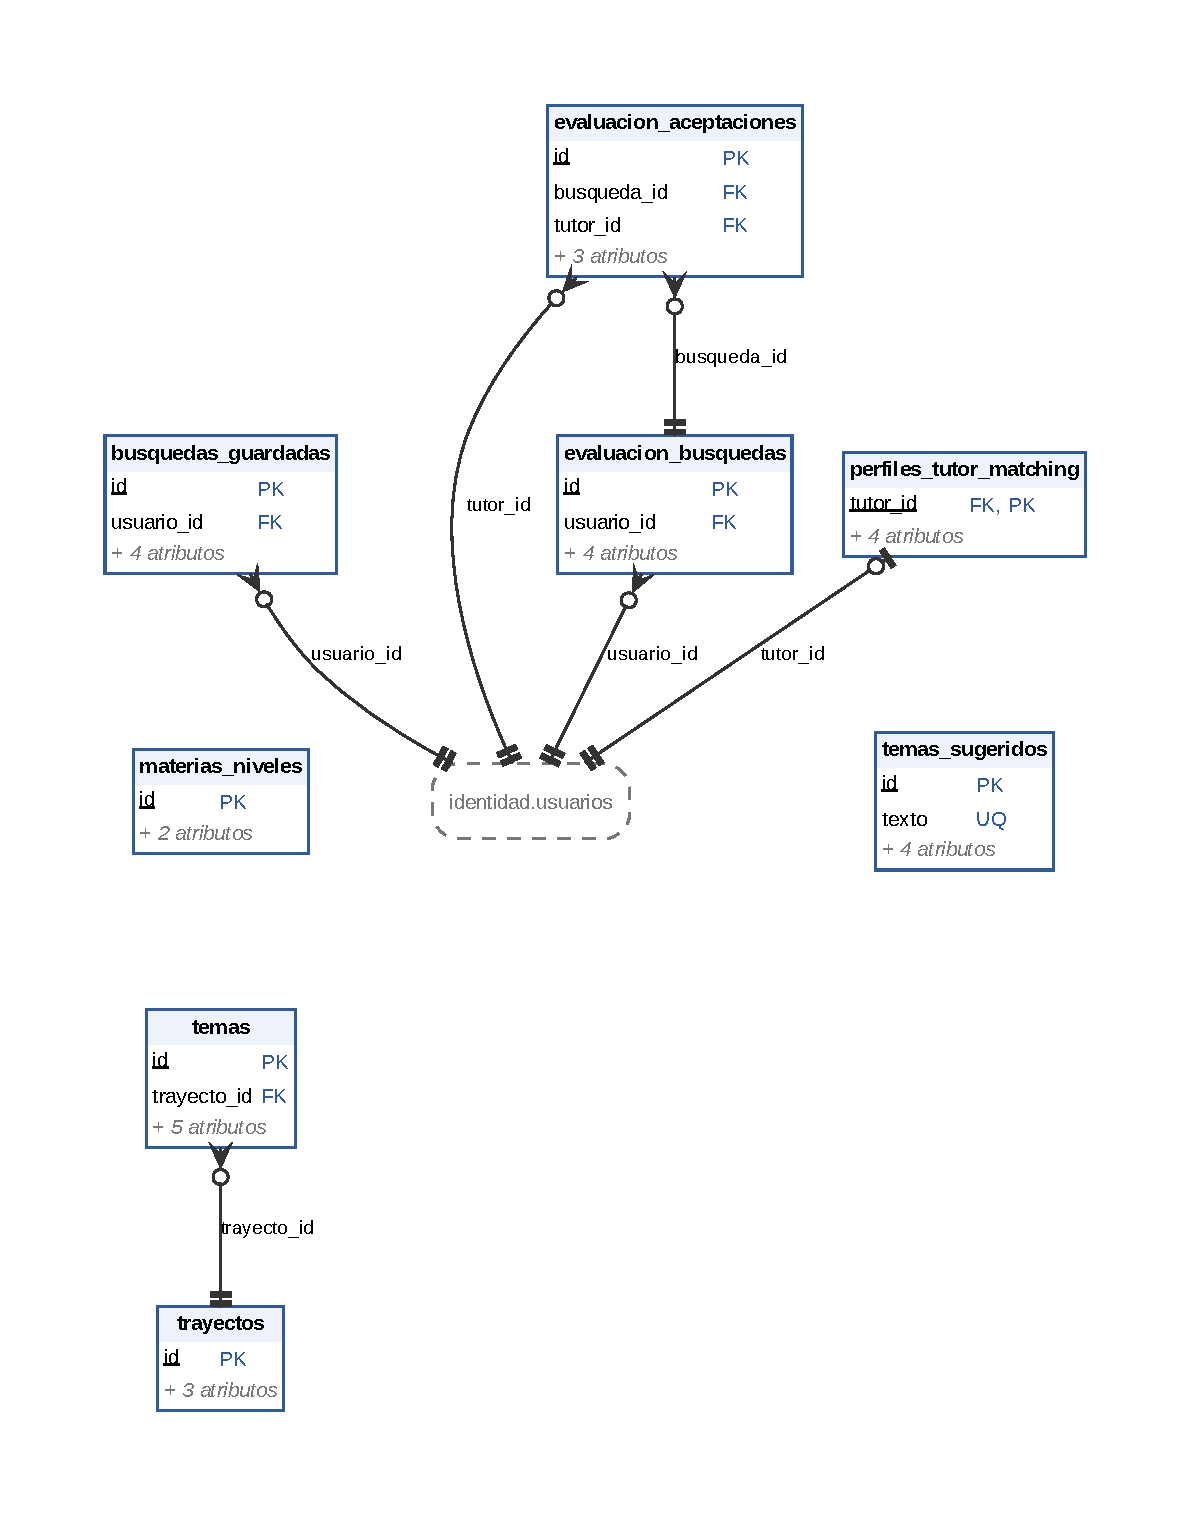
\includegraphics[scale=0.744]{figuras/der/matching}
    \caption{Diagrama entidad-relación del esquema \texttt{matching} (M2)}
    \label{fig:der-matching}
\end{figure}

\subsubsection{\texorpdfstring{\texttt{matching.busquedas\_\allowbreak{}guardadas}}{matching.busquedas\_guardadas}}\label{dd:matching.busquedas_guardadas}

Búsquedas que el usuario guarda para volver a ejecutar; se guardan la consulta y los filtros, nunca la lista de resultados. \emph{Migraciones:} V7, V49.

{\small
\begin{xltabular}{\textwidth}{@{}>{\raggedright\arraybackslash}p{3.6cm} >{\raggedright\arraybackslash}p{2.3cm} >{\raggedright\arraybackslash}p{1cm} >{\centering\arraybackslash}p{0.85cm} L@{}}
    \toprule
    \tb{Atributo} & \tb{Tipo} & \tb{Clave} & \tb{Nulo} & \tb{Descripción} \\
    \midrule
    \endfirsthead
    \toprule
    \tb{Atributo} & \tb{Tipo} & \tb{Clave} & \tb{Nulo} & \tb{Descripción} \\
    \midrule
    \endhead
    \bottomrule
    \endfoot
    \texttt{id} & \texttt{uuid} & PK & no & Identificador (UUID generado por la base) \\
    \texttt{usuario\_\allowbreak{}id} & \texttt{uuid} & FK & no & Usuario que guardó la búsqueda \\
    \texttt{texto\_\allowbreak{}busqueda} & \texttt{varchar(\allowbreak{}500)} &  & no & Texto libre de la consulta \\
    \texttt{created\_\allowbreak{}at} & \texttt{timestamptz} &  & no & Fecha y hora de creación de la fila. Por defecto: \texttt{now(\allowbreak{})} \\
    \texttt{filtros} & \texttt{jsonb} &  & no & Filtros aplicados (nivel, materia, nombre, precio máximo) en JSON. Por defecto: \texttt{\textquotesingle{}\{\}\textquotesingle{}} \\
    \texttt{huella} & \texttt{varchar(\allowbreak{}64)} &  & no & SHA-256 del texto normalizado y los filtros ordenados; impide guardar dos veces la misma búsqueda \\
\end{xltabular}
}

{\small
\begin{xltabular}{\textwidth}{@{}>{\raggedright\arraybackslash}p{1.7cm} >{\raggedright\arraybackslash}p{4.6cm} L@{}}
    \toprule
    \tb{Tipo} & \tb{Nombre} & \tb{Definición} \\
    \midrule
    \endfirsthead
    \toprule
    \tb{Tipo} & \tb{Nombre} & \tb{Definición} \\
    \midrule
    \endhead
    \bottomrule
    \endfoot
    FK & \texttt{busquedas\_\allowbreak{}guardadas\_\allowbreak{}usuario\_\allowbreak{}id\_\allowbreak{}fkey} & \texttt{(\allowbreak{}usuario\_\allowbreak{}id) $\rightarrow$ identidad.usuarios(\allowbreak{}id)} \\
    PK & \texttt{busquedas\_\allowbreak{}guardadas\_\allowbreak{}pkey} & \texttt{(\allowbreak{}id)} \\
    Índice & \texttt{idx\_\allowbreak{}busquedas\_\allowbreak{}guardadas\_\allowbreak{}usuario} & \texttt{(\allowbreak{}usuario\_\allowbreak{}id)} \\
    UNIQUE & \texttt{uq\_\allowbreak{}busquedas\_\allowbreak{}guardadas\_\allowbreak{}usuario\_\allowbreak{}huella} & \texttt{(\allowbreak{}usuario\_\allowbreak{}id,\allowbreak{} huella)} \\
\end{xltabular}
}

\subsubsection{\texorpdfstring{\texttt{matching.evaluacion\_\allowbreak{}aceptaciones}}{matching.evaluacion\_aceptaciones}}\label{dd:matching.evaluacion_aceptaciones}

Instrumentación de la evaluación (I-01): el usuario abrió el perfil o reservó a un tutor sugerido en una búsqueda registrada. \emph{Migraciones:} V58.

{\small
\begin{xltabular}{\textwidth}{@{}>{\raggedright\arraybackslash}p{3.6cm} >{\raggedright\arraybackslash}p{2.3cm} >{\raggedright\arraybackslash}p{1cm} >{\centering\arraybackslash}p{0.85cm} L@{}}
    \toprule
    \tb{Atributo} & \tb{Tipo} & \tb{Clave} & \tb{Nulo} & \tb{Descripción} \\
    \midrule
    \endfirsthead
    \toprule
    \tb{Atributo} & \tb{Tipo} & \tb{Clave} & \tb{Nulo} & \tb{Descripción} \\
    \midrule
    \endhead
    \bottomrule
    \endfoot
    \texttt{id} & \texttt{uuid} & PK & no & Identificador (UUID generado por la base) \\
    \texttt{busqueda\_\allowbreak{}id} & \texttt{uuid} & FK & no & Búsqueda registrada en la que apareció el tutor \\
    \texttt{tutor\_\allowbreak{}id} & \texttt{uuid} & FK & no & Tutor aceptado \\
    \texttt{posicion} & \texttt{integer} &  & no & Posición del tutor en el ranking (1 es el primero); la calcula el servidor \\
    \texttt{tipo} & \texttt{varchar(\allowbreak{}10)} &  & no & PERFIL (abrió el perfil) o RESERVA (reservó) \\
    \texttt{created\_\allowbreak{}at} & \texttt{timestamptz} &  & no & Fecha y hora de la aceptación. Por defecto: \texttt{now(\allowbreak{})} \\
\end{xltabular}
}

{\small
\begin{xltabular}{\textwidth}{@{}>{\raggedright\arraybackslash}p{1.7cm} >{\raggedright\arraybackslash}p{4.6cm} L@{}}
    \toprule
    \tb{Tipo} & \tb{Nombre} & \tb{Definición} \\
    \midrule
    \endfirsthead
    \toprule
    \tb{Tipo} & \tb{Nombre} & \tb{Definición} \\
    \midrule
    \endhead
    \bottomrule
    \endfoot
    CHECK & \texttt{evaluacion\_\allowbreak{}aceptaciones\_\allowbreak{}posicion\_\allowbreak{}check} & \texttt{posicion \textgreater{}= 1} \\
    CHECK & \texttt{evaluacion\_\allowbreak{}aceptaciones\_\allowbreak{}tipo\_\allowbreak{}check} & \texttt{tipo IN (\allowbreak{}\textquotesingle{}PERFIL\textquotesingle{},\allowbreak{} \textquotesingle{}RESERVA\textquotesingle{})} \\
    FK & \texttt{evaluacion\_\allowbreak{}aceptaciones\_\allowbreak{}busqueda\_\allowbreak{}id\_\allowbreak{}fkey} & \texttt{(\allowbreak{}busqueda\_\allowbreak{}id) $\rightarrow$ matching.evaluacion\_\allowbreak{}busquedas(\allowbreak{}id)} \texttt{ON DELETE CASCADE} \\
    FK & \texttt{evaluacion\_\allowbreak{}aceptaciones\_\allowbreak{}tutor\_\allowbreak{}id\_\allowbreak{}fkey} & \texttt{(\allowbreak{}tutor\_\allowbreak{}id) $\rightarrow$ identidad.usuarios(\allowbreak{}id)} \\
    PK & \texttt{evaluacion\_\allowbreak{}aceptaciones\_\allowbreak{}pkey} & \texttt{(\allowbreak{}id)} \\
    UNIQUE & \texttt{uq\_\allowbreak{}evaluacion\_\allowbreak{}aceptacion} & \texttt{(\allowbreak{}busqueda\_\allowbreak{}id,\allowbreak{} tutor\_\allowbreak{}id,\allowbreak{} tipo)} \\
\end{xltabular}
}

\subsubsection{\texorpdfstring{\texttt{matching.evaluacion\_\allowbreak{}busquedas}}{matching.evaluacion\_busquedas}}\label{dd:matching.evaluacion_busquedas}

Instrumentación de la evaluación del \gls{matching} (indicador I-01): qué tutores se mostraron y en qué orden. No guarda el texto buscado ni las búsquedas de menores. Solo se escribe con \path{tinku.evaluacion.habilitada}. \emph{Migraciones:} V58.

{\small
\begin{xltabular}{\textwidth}{@{}>{\raggedright\arraybackslash}p{3.6cm} >{\raggedright\arraybackslash}p{2.3cm} >{\raggedright\arraybackslash}p{1cm} >{\centering\arraybackslash}p{0.85cm} L@{}}
    \toprule
    \tb{Atributo} & \tb{Tipo} & \tb{Clave} & \tb{Nulo} & \tb{Descripción} \\
    \midrule
    \endfirsthead
    \toprule
    \tb{Atributo} & \tb{Tipo} & \tb{Clave} & \tb{Nulo} & \tb{Descripción} \\
    \midrule
    \endhead
    \bottomrule
    \endfoot
    \texttt{id} & \texttt{uuid} & PK & no & Identificador (UUID generado por la base) \\
    \texttt{usuario\_\allowbreak{}id} & \texttt{uuid} & FK & no & Usuario que buscó \\
    \texttt{longitud\_\allowbreak{}texto} & \texttt{integer} &  & no & Longitud del texto buscado, en caracteres \\
    \texttt{cantidad\_\allowbreak{}resultados} & \texttt{integer} &  & no & Cantidad de tutores devueltos \\
    \texttt{tutor\_\allowbreak{}ids} & \texttt{uuid[]} &  & no & Tutores mostrados, en el orden del ranking \\
    \texttt{created\_\allowbreak{}at} & \texttt{timestamptz} &  & no & Fecha y hora de la búsqueda. Por defecto: \texttt{now(\allowbreak{})} \\
\end{xltabular}
}

{\small
\begin{xltabular}{\textwidth}{@{}>{\raggedright\arraybackslash}p{1.7cm} >{\raggedright\arraybackslash}p{4.6cm} L@{}}
    \toprule
    \tb{Tipo} & \tb{Nombre} & \tb{Definición} \\
    \midrule
    \endfirsthead
    \toprule
    \tb{Tipo} & \tb{Nombre} & \tb{Definición} \\
    \midrule
    \endhead
    \bottomrule
    \endfoot
    CHECK & \texttt{evaluacion\_\allowbreak{}busquedas\_\allowbreak{}cantidad\_\allowbreak{}resultados\_\allowbreak{}check} & \texttt{cantidad\_\allowbreak{}resultados \textgreater{}= 0} \\
    CHECK & \texttt{evaluacion\_\allowbreak{}busquedas\_\allowbreak{}longitud\_\allowbreak{}texto\_\allowbreak{}check} & \texttt{longitud\_\allowbreak{}texto \textgreater{}= 0} \\
    FK & \texttt{evaluacion\_\allowbreak{}busquedas\_\allowbreak{}usuario\_\allowbreak{}id\_\allowbreak{}fkey} & \texttt{(\allowbreak{}usuario\_\allowbreak{}id) $\rightarrow$ identidad.usuarios(\allowbreak{}id)} \\
    PK & \texttt{evaluacion\_\allowbreak{}busquedas\_\allowbreak{}pkey} & \texttt{(\allowbreak{}id)} \\
    Índice & \texttt{idx\_\allowbreak{}evaluacion\_\allowbreak{}busquedas\_\allowbreak{}created} & \texttt{(\allowbreak{}created\_\allowbreak{}at)} \\
\end{xltabular}
}

\subsubsection{\texorpdfstring{\texttt{matching.materias\_\allowbreak{}niveles}}{matching.materias\_niveles}}\label{dd:matching.materias_niveles}

Catálogo inicial de materias por nivel (V7). Lo reemplazó el catálogo de trayectos y temas (V19); solo lo usa el endpoint heredado \path{PUT /api/perfil-matching}. \emph{Migraciones:} V7.

{\small
\begin{xltabular}{\textwidth}{@{}>{\raggedright\arraybackslash}p{3.6cm} >{\raggedright\arraybackslash}p{2.3cm} >{\raggedright\arraybackslash}p{1cm} >{\centering\arraybackslash}p{0.85cm} L@{}}
    \toprule
    \tb{Atributo} & \tb{Tipo} & \tb{Clave} & \tb{Nulo} & \tb{Descripción} \\
    \midrule
    \endfirsthead
    \toprule
    \tb{Atributo} & \tb{Tipo} & \tb{Clave} & \tb{Nulo} & \tb{Descripción} \\
    \midrule
    \endhead
    \bottomrule
    \endfoot
    \texttt{id} & \texttt{uuid} & PK & no & Identificador (UUID generado por la base) \\
    \texttt{nivel} & \texttt{varchar(\allowbreak{}20)} &  & no & primario, secundario o universitario \\
    \texttt{materia} & \texttt{varchar(\allowbreak{}100)} &  & no & Nombre de la materia \\
\end{xltabular}
}

{\small
\begin{xltabular}{\textwidth}{@{}>{\raggedright\arraybackslash}p{1.7cm} >{\raggedright\arraybackslash}p{4.6cm} L@{}}
    \toprule
    \tb{Tipo} & \tb{Nombre} & \tb{Definición} \\
    \midrule
    \endfirsthead
    \toprule
    \tb{Tipo} & \tb{Nombre} & \tb{Definición} \\
    \midrule
    \endhead
    \bottomrule
    \endfoot
    CHECK & \texttt{materias\_\allowbreak{}niveles\_\allowbreak{}nivel\_\allowbreak{}check} & \texttt{nivel IN (\allowbreak{}\textquotesingle{}primario\textquotesingle{},\allowbreak{} \textquotesingle{}secundario\textquotesingle{},\allowbreak{} \textquotesingle{}universitario\textquotesingle{})} \\
    PK & \texttt{materias\_\allowbreak{}niveles\_\allowbreak{}pkey} & \texttt{(\allowbreak{}id)} \\
    UNIQUE & \texttt{uq\_\allowbreak{}materia\_\allowbreak{}nivel} & \texttt{(\allowbreak{}nivel,\allowbreak{} materia)} \\
    Índice & \texttt{idx\_\allowbreak{}materias\_\allowbreak{}niveles\_\allowbreak{}nivel} & \texttt{(\allowbreak{}nivel)} \\
\end{xltabular}
}

\subsubsection{\texorpdfstring{\texttt{matching.perfiles\_\allowbreak{}tutor\_\allowbreak{}matching}}{matching.perfiles\_tutor\_matching}}\label{dd:matching.perfiles_tutor_matching}

Perfil del tutor para el motor de \gls{matching}: temas elegidos y \gls{embeddings} del perfil. \emph{Migraciones:} V7, V19.

{\small
\begin{xltabular}{\textwidth}{@{}>{\raggedright\arraybackslash}p{3.6cm} >{\raggedright\arraybackslash}p{2.3cm} >{\raggedright\arraybackslash}p{1cm} >{\centering\arraybackslash}p{0.85cm} L@{}}
    \toprule
    \tb{Atributo} & \tb{Tipo} & \tb{Clave} & \tb{Nulo} & \tb{Descripción} \\
    \midrule
    \endfirsthead
    \toprule
    \tb{Atributo} & \tb{Tipo} & \tb{Clave} & \tb{Nulo} & \tb{Descripción} \\
    \midrule
    \endhead
    \bottomrule
    \endfoot
    \texttt{tutor\_\allowbreak{}id} & \texttt{uuid} & FK, PK & no & Tutor al que pertenece el perfil \\
    \texttt{materias\_\allowbreak{}niveles\_\allowbreak{}ids} & \texttt{uuid[]} &  & no & Materias del catálogo inicial; arreglo sin clave foránea, solo lo llena el endpoint heredado. Por defecto: \texttt{\textquotesingle{}\{\}\textquotesingle{}} \\
    \texttt{embedding} & \texttt{vector(\allowbreak{}384)} &  & sí & \gls{embeddings} del perfil completo (384 dimensiones); se usa solo si ninguno de sus temas tiene \gls{embeddings} \\
    \texttt{activo\_\allowbreak{}para\_\allowbreak{}matching} & \texttt{boolean} &  & no & Bandera de V7; el filtro que se aplica es \path{identidad.usuarios.activo_para_matching}. Por defecto: \texttt{false} \\
    \texttt{tema\_\allowbreak{}ids} & \texttt{uuid[]} &  & no & Temas del catálogo elegidos por el tutor; arreglo sin clave foránea, con índice GIN. Por defecto: \texttt{\textquotesingle{}\{\}\textquotesingle{}} \\
\end{xltabular}
}

{\small
\begin{xltabular}{\textwidth}{@{}>{\raggedright\arraybackslash}p{1.7cm} >{\raggedright\arraybackslash}p{4.6cm} L@{}}
    \toprule
    \tb{Tipo} & \tb{Nombre} & \tb{Definición} \\
    \midrule
    \endfirsthead
    \toprule
    \tb{Tipo} & \tb{Nombre} & \tb{Definición} \\
    \midrule
    \endhead
    \bottomrule
    \endfoot
    FK & \texttt{perfiles\_\allowbreak{}tutor\_\allowbreak{}matching\_\allowbreak{}tutor\_\allowbreak{}id\_\allowbreak{}fkey} & \texttt{(\allowbreak{}tutor\_\allowbreak{}id) $\rightarrow$ identidad.usuarios(\allowbreak{}id)} \\
    PK & \texttt{perfiles\_\allowbreak{}tutor\_\allowbreak{}matching\_\allowbreak{}pkey} & \texttt{(\allowbreak{}tutor\_\allowbreak{}id)} \\
    Índice & \texttt{idx\_\allowbreak{}perfiles\_\allowbreak{}tutor\_\allowbreak{}matching\_\allowbreak{}tema\_\allowbreak{}ids} & \texttt{(\allowbreak{}tema\_\allowbreak{}ids) USING gin} \\
\end{xltabular}
}

\subsubsection{\texorpdfstring{\texttt{matching.temas}}{matching.temas}}\label{dd:matching.temas}

Temas de cada trayecto: la unidad que elige el tutor y con la que se calcula la similitud de una búsqueda (ADR-M2-03). \emph{Migraciones:} V19, V20, V42.

{\small
\begin{xltabular}{\textwidth}{@{}>{\raggedright\arraybackslash}p{3.6cm} >{\raggedright\arraybackslash}p{2.3cm} >{\raggedright\arraybackslash}p{1cm} >{\centering\arraybackslash}p{0.85cm} L@{}}
    \toprule
    \tb{Atributo} & \tb{Tipo} & \tb{Clave} & \tb{Nulo} & \tb{Descripción} \\
    \midrule
    \endfirsthead
    \toprule
    \tb{Atributo} & \tb{Tipo} & \tb{Clave} & \tb{Nulo} & \tb{Descripción} \\
    \midrule
    \endhead
    \bottomrule
    \endfoot
    \texttt{id} & \texttt{uuid} & PK & no & Identificador (UUID generado por la base) \\
    \texttt{trayecto\_\allowbreak{}id} & \texttt{uuid} & FK & no & Trayecto al que pertenece el tema \\
    \texttt{nombre} & \texttt{text} &  & no & Nombre del tema \\
    \texttt{descripcion} & \texttt{text} &  & no & Qué se trabaja en el tema; es el texto que se convierte en \gls{embeddings} \\
    \texttt{orden} & \texttt{integer} &  & no & Posición del tema dentro del trayecto. Por defecto: \texttt{0} \\
    \texttt{embedding} & \texttt{vector(\allowbreak{}384)} &  & sí & \gls{embeddings} del tema (384 dimensiones); nulo si ningún tutor lo eligió todavía \\
    \texttt{embedding\_\allowbreak{}fuente} & \texttt{text} &  & sí & Texto con el que se calculó el \gls{embeddings}; si cambia, se recalcula \\
\end{xltabular}
}

{\small
\begin{xltabular}{\textwidth}{@{}>{\raggedright\arraybackslash}p{1.7cm} >{\raggedright\arraybackslash}p{4.6cm} L@{}}
    \toprule
    \tb{Tipo} & \tb{Nombre} & \tb{Definición} \\
    \midrule
    \endfirsthead
    \toprule
    \tb{Tipo} & \tb{Nombre} & \tb{Definición} \\
    \midrule
    \endhead
    \bottomrule
    \endfoot
    FK & \texttt{temas\_\allowbreak{}trayecto\_\allowbreak{}id\_\allowbreak{}fkey} & \texttt{(\allowbreak{}trayecto\_\allowbreak{}id) $\rightarrow$ matching.trayectos(\allowbreak{}id)} \\
    PK & \texttt{temas\_\allowbreak{}pkey} & \texttt{(\allowbreak{}id)} \\
    UNIQUE & \texttt{uq\_\allowbreak{}tema} & \texttt{(\allowbreak{}trayecto\_\allowbreak{}id,\allowbreak{} nombre)} \\
\end{xltabular}
}

\subsubsection{\texorpdfstring{\texttt{matching.temas\_\allowbreak{}sugeridos}}{matching.temas\_sugeridos}}\label{dd:matching.temas_sugeridos}

Contador agregado de temas buscados que el catálogo no cubre (ADR-M2-04). No guarda quién buscó ni una fila por búsqueda, y excluye las búsquedas de menores. El servicio la mantiene en 500 filas como máximo. \emph{Migraciones:} V43.

{\small
\begin{xltabular}{\textwidth}{@{}>{\raggedright\arraybackslash}p{3.6cm} >{\raggedright\arraybackslash}p{2.3cm} >{\raggedright\arraybackslash}p{1cm} >{\centering\arraybackslash}p{0.85cm} L@{}}
    \toprule
    \tb{Atributo} & \tb{Tipo} & \tb{Clave} & \tb{Nulo} & \tb{Descripción} \\
    \midrule
    \endfirsthead
    \toprule
    \tb{Atributo} & \tb{Tipo} & \tb{Clave} & \tb{Nulo} & \tb{Descripción} \\
    \midrule
    \endhead
    \bottomrule
    \endfoot
    \texttt{id} & \texttt{uuid} & PK & no & Identificador (UUID generado por la base) \\
    \texttt{texto} & \texttt{text} & UQ & no & Texto de búsqueda normalizado \\
    \texttt{veces} & \texttt{integer} &  & no & Cantidad de veces que se buscó. Por defecto: \texttt{1} \\
    \texttt{nivel} & \texttt{text} &  & sí & Nivel del tema del catálogo más parecido \\
    \texttt{materia} & \texttt{text} &  & sí & Materia del tema del catálogo más parecido \\
    \texttt{ultima\_\allowbreak{}vez} & \texttt{timestamptz} &  & no & Fecha y hora de la última búsqueda. Por defecto: \texttt{now(\allowbreak{})} \\
\end{xltabular}
}

{\small
\begin{xltabular}{\textwidth}{@{}>{\raggedright\arraybackslash}p{1.7cm} >{\raggedright\arraybackslash}p{4.6cm} L@{}}
    \toprule
    \tb{Tipo} & \tb{Nombre} & \tb{Definición} \\
    \midrule
    \endfirsthead
    \toprule
    \tb{Tipo} & \tb{Nombre} & \tb{Definición} \\
    \midrule
    \endhead
    \bottomrule
    \endfoot
    PK & \texttt{temas\_\allowbreak{}sugeridos\_\allowbreak{}pkey} & \texttt{(\allowbreak{}id)} \\
    UNIQUE & \texttt{temas\_\allowbreak{}sugeridos\_\allowbreak{}texto\_\allowbreak{}key} & \texttt{(\allowbreak{}texto)} \\
    Índice & \texttt{idx\_\allowbreak{}temas\_\allowbreak{}sugeridos\_\allowbreak{}veces} & \texttt{(\allowbreak{}veces DESC,\allowbreak{} ultima\_\allowbreak{}vez DESC)} \\
\end{xltabular}
}

\subsubsection{\texorpdfstring{\texttt{matching.trayectos}}{matching.trayectos}}\label{dd:matching.trayectos}

Catálogo cerrado de trayectos: nivel, año o carrera y materia. Lo siembra \path{V20__m2_temas_seed.sql}. \emph{Migraciones:} V19, V20.

{\small
\begin{xltabular}{\textwidth}{@{}>{\raggedright\arraybackslash}p{3.6cm} >{\raggedright\arraybackslash}p{2.3cm} >{\raggedright\arraybackslash}p{1cm} >{\centering\arraybackslash}p{0.85cm} L@{}}
    \toprule
    \tb{Atributo} & \tb{Tipo} & \tb{Clave} & \tb{Nulo} & \tb{Descripción} \\
    \midrule
    \endfirsthead
    \toprule
    \tb{Atributo} & \tb{Tipo} & \tb{Clave} & \tb{Nulo} & \tb{Descripción} \\
    \midrule
    \endhead
    \bottomrule
    \endfoot
    \texttt{id} & \texttt{uuid} & PK & no & Identificador (UUID generado por la base) \\
    \texttt{nivel} & \texttt{text} &  & no & primario, secundario o universitario \\
    \texttt{anio\_\allowbreak{}o\_\allowbreak{}carrera} & \texttt{text} &  & no & Año o curso (por ejemplo, ``4°'') o carrera \\
    \texttt{materia} & \texttt{text} &  & no & Nombre de la materia \\
\end{xltabular}
}

{\small
\begin{xltabular}{\textwidth}{@{}>{\raggedright\arraybackslash}p{1.7cm} >{\raggedright\arraybackslash}p{4.6cm} L@{}}
    \toprule
    \tb{Tipo} & \tb{Nombre} & \tb{Definición} \\
    \midrule
    \endfirsthead
    \toprule
    \tb{Tipo} & \tb{Nombre} & \tb{Definición} \\
    \midrule
    \endhead
    \bottomrule
    \endfoot
    CHECK & \texttt{trayectos\_\allowbreak{}nivel\_\allowbreak{}check} & \texttt{nivel IN (\allowbreak{}\textquotesingle{}primario\textquotesingle{},\allowbreak{} \textquotesingle{}secundario\textquotesingle{},\allowbreak{} \textquotesingle{}universitario\textquotesingle{})} \\
    PK & \texttt{trayectos\_\allowbreak{}pkey} & \texttt{(\allowbreak{}id)} \\
    UNIQUE & \texttt{uq\_\allowbreak{}trayecto} & \texttt{(\allowbreak{}nivel,\allowbreak{} anio\_\allowbreak{}o\_\allowbreak{}carrera,\allowbreak{} materia)} \\
\end{xltabular}
}

\subsection{Esquema \texttt{aula} (M3)}\label{dd:aula}

Aula virtual: sesión de clase asociada a cada reserva, alertas del kill-switch y confirmación de la contraparte en la rama de adultos. Tablas: 3. Su diagrama entidad-relación es la figura~\ref{fig:der-aula}.

\begin{figure}[htbp]
    \centering
    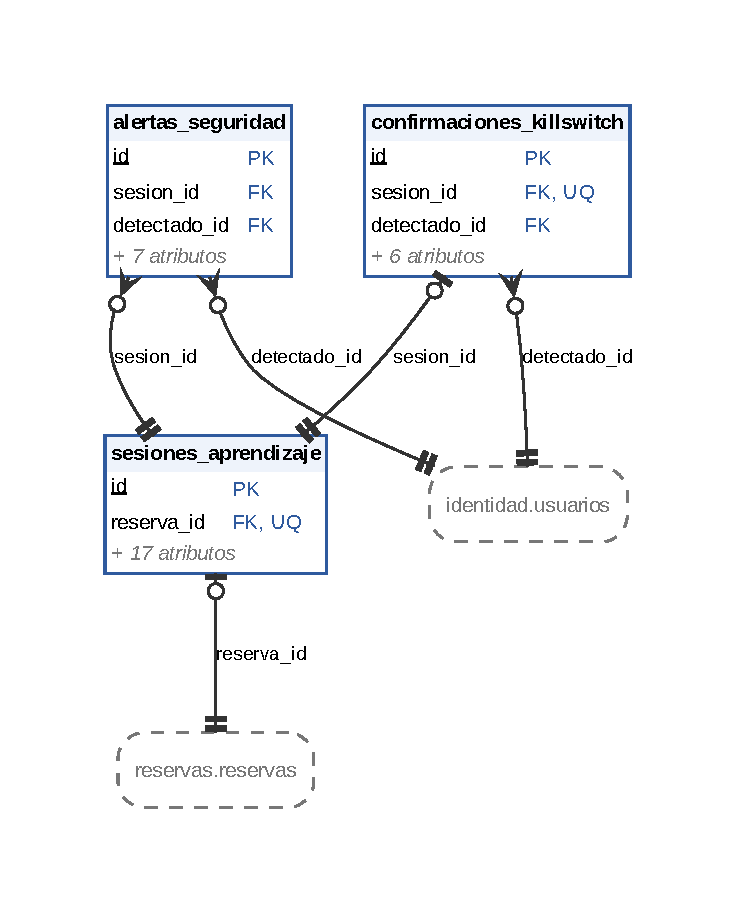
\includegraphics[scale=1.000]{figuras/der/aula}
    \caption{Diagrama entidad-relación del esquema \texttt{aula} (M3)}
    \label{fig:der-aula}
\end{figure}

\subsubsection{\texorpdfstring{\texttt{aula.alertas\_\allowbreak{}seguridad}}{aula.alertas\_seguridad}}\label{dd:aula.alertas_seguridad}

Alerta del kill-switch. Es una entidad distinta de la denuncia: la revisa moderación dentro de 12 horas, sin esperar descargo. \emph{Migraciones:} V8, V13.

{\small
\begin{xltabular}{\textwidth}{@{}>{\raggedright\arraybackslash}p{3.6cm} >{\raggedright\arraybackslash}p{2.3cm} >{\raggedright\arraybackslash}p{1cm} >{\centering\arraybackslash}p{0.85cm} L@{}}
    \toprule
    \tb{Atributo} & \tb{Tipo} & \tb{Clave} & \tb{Nulo} & \tb{Descripción} \\
    \midrule
    \endfirsthead
    \toprule
    \tb{Atributo} & \tb{Tipo} & \tb{Clave} & \tb{Nulo} & \tb{Descripción} \\
    \midrule
    \endhead
    \bottomrule
    \endfoot
    \texttt{id} & \texttt{uuid} & PK & no & Identificador (UUID generado por la base) \\
    \texttt{sesion\_\allowbreak{}id} & \texttt{uuid} & FK & no & Sesión en la que se detectó el contenido \\
    \texttt{rama} & \texttt{varchar(\allowbreak{}10)} &  & no & menor o adultos; la decide el backend con datos de M1, nunca el cliente \\
    \texttt{detectado\_\allowbreak{}id} & \texttt{uuid} & FK & no & Usuario cuyo video disparó la detección \\
    \texttt{clip\_\allowbreak{}url} & \texttt{varchar(\allowbreak{}500)} &  & sí & Referencia al clip de evidencia \\
    \texttt{clip\_\allowbreak{}retencion\_\allowbreak{}hasta} & \texttt{timestamptz} &  & sí & Fin de la retención del clip: 30 días desde la resolución \\
    \texttt{estado} & \texttt{varchar(\allowbreak{}30)} &  & no & Estado de la revisión. Por defecto: \texttt{\textquotesingle{}pendiente\_\allowbreak{}revision\textquotesingle{}} \\
    \texttt{created\_\allowbreak{}at} & \texttt{timestamptz} &  & no & Fecha y hora de la detección. Por defecto: \texttt{now(\allowbreak{})} \\
    \texttt{descargo\_\allowbreak{}texto} & \texttt{varchar(\allowbreak{}300)} &  & sí & Descargo del usuario detectado (hasta 300 caracteres); no bloquea la resolución \\
    \texttt{descargo\_\allowbreak{}recibido\_\allowbreak{}at} & \texttt{timestamptz} &  & sí & Fecha y hora del descargo \\
\end{xltabular}
}

{\small
\begin{xltabular}{\textwidth}{@{}>{\raggedright\arraybackslash}p{1.7cm} >{\raggedright\arraybackslash}p{4.6cm} L@{}}
    \toprule
    \tb{Tipo} & \tb{Nombre} & \tb{Definición} \\
    \midrule
    \endfirsthead
    \toprule
    \tb{Tipo} & \tb{Nombre} & \tb{Definición} \\
    \midrule
    \endhead
    \bottomrule
    \endfoot
    CHECK & \texttt{alertas\_\allowbreak{}seguridad\_\allowbreak{}estado\_\allowbreak{}check} & \texttt{estado IN (\allowbreak{}\textquotesingle{}pendiente\_\allowbreak{}revision\textquotesingle{},\allowbreak{} \textquotesingle{}resuelta\_\allowbreak{}reactivacion\textquotesingle{},\allowbreak{} \textquotesingle{}resuelta\_\allowbreak{}baja\textquotesingle{})} \\
    CHECK & \texttt{alertas\_\allowbreak{}seguridad\_\allowbreak{}rama\_\allowbreak{}check} & \texttt{rama IN (\allowbreak{}\textquotesingle{}menor\textquotesingle{},\allowbreak{} \textquotesingle{}adultos\textquotesingle{})} \\
    FK & \texttt{alertas\_\allowbreak{}seguridad\_\allowbreak{}detectado\_\allowbreak{}id\_\allowbreak{}fkey} & \texttt{(\allowbreak{}detectado\_\allowbreak{}id) $\rightarrow$ identidad.usuarios(\allowbreak{}id)} \\
    FK & \texttt{alertas\_\allowbreak{}seguridad\_\allowbreak{}sesion\_\allowbreak{}id\_\allowbreak{}fkey} & \texttt{(\allowbreak{}sesion\_\allowbreak{}id) $\rightarrow$ aula.sesiones\_\allowbreak{}aprendizaje(\allowbreak{}id)} \\
    PK & \texttt{alertas\_\allowbreak{}seguridad\_\allowbreak{}pkey} & \texttt{(\allowbreak{}id)} \\
    Índice & \texttt{idx\_\allowbreak{}alertas\_\allowbreak{}seguridad\_\allowbreak{}estado} & \texttt{(\allowbreak{}estado)} \\
    Índice & \texttt{idx\_\allowbreak{}alertas\_\allowbreak{}seguridad\_\allowbreak{}sesion} & \texttt{(\allowbreak{}sesion\_\allowbreak{}id)} \\
\end{xltabular}
}

\subsubsection{\texorpdfstring{\texttt{aula.confirmaciones\_\allowbreak{}killswitch}}{aula.confirmaciones\_killswitch}}\label{dd:aula.confirmaciones_killswitch}

Pregunta a la contraparte en la rama de adultos del kill-switch, antes de cortar la clase (ADR-M3-07). Sin respuesta en plazo, cuenta como ``No''. \emph{Migraciones:} V12, V47.

{\small
\begin{xltabular}{\textwidth}{@{}>{\raggedright\arraybackslash}p{3.6cm} >{\raggedright\arraybackslash}p{2.3cm} >{\raggedright\arraybackslash}p{1cm} >{\centering\arraybackslash}p{0.85cm} L@{}}
    \toprule
    \tb{Atributo} & \tb{Tipo} & \tb{Clave} & \tb{Nulo} & \tb{Descripción} \\
    \midrule
    \endfirsthead
    \toprule
    \tb{Atributo} & \tb{Tipo} & \tb{Clave} & \tb{Nulo} & \tb{Descripción} \\
    \midrule
    \endhead
    \bottomrule
    \endfoot
    \texttt{id} & \texttt{uuid} & PK & no & Identificador (UUID generado por la base) \\
    \texttt{sesion\_\allowbreak{}id} & \texttt{uuid} & FK, UQ & no & Sesión en la que se hizo la pregunta (una por sesión) \\
    \texttt{detectado\_\allowbreak{}id} & \texttt{uuid} & FK & no & Usuario cuyo video disparó la detección \\
    \texttt{respondido\_\allowbreak{}id} & \texttt{uuid} &  & sí & Usuario que respondió; nulo mientras se espera la respuesta \\
    \texttt{vio} & \texttt{boolean} &  & sí & Respuesta: si la contraparte vio el contenido; nula hasta que responda \\
    \texttt{created\_\allowbreak{}at} & \texttt{timestamptz} &  & no & Fecha y hora de la pregunta. Por defecto: \texttt{now(\allowbreak{})} \\
    \texttt{responded\_\allowbreak{}at} & \texttt{timestamptz} &  & sí & Fecha y hora de la respuesta \\
    \texttt{vence\_\allowbreak{}at} & \texttt{timestamptz} &  & sí & Fin del plazo para responder \\
    \texttt{vencida} & \texttt{boolean} &  & no & El plazo venció sin respuesta. Por defecto: \texttt{false} \\
\end{xltabular}
}

{\small
\begin{xltabular}{\textwidth}{@{}>{\raggedright\arraybackslash}p{1.7cm} >{\raggedright\arraybackslash}p{4.6cm} L@{}}
    \toprule
    \tb{Tipo} & \tb{Nombre} & \tb{Definición} \\
    \midrule
    \endfirsthead
    \toprule
    \tb{Tipo} & \tb{Nombre} & \tb{Definición} \\
    \midrule
    \endhead
    \bottomrule
    \endfoot
    FK & \texttt{confirmaciones\_\allowbreak{}killswitch\_\allowbreak{}detectado\_\allowbreak{}id\_\allowbreak{}fkey} & \texttt{(\allowbreak{}detectado\_\allowbreak{}id) $\rightarrow$ identidad.usuarios(\allowbreak{}id)} \\
    FK & \texttt{confirmaciones\_\allowbreak{}killswitch\_\allowbreak{}sesion\_\allowbreak{}id\_\allowbreak{}fkey} & \texttt{(\allowbreak{}sesion\_\allowbreak{}id) $\rightarrow$ aula.sesiones\_\allowbreak{}aprendizaje(\allowbreak{}id)} \\
    PK & \texttt{confirmaciones\_\allowbreak{}killswitch\_\allowbreak{}pkey} & \texttt{(\allowbreak{}id)} \\
    UNIQUE & \texttt{confirmaciones\_\allowbreak{}killswitch\_\allowbreak{}sesion\_\allowbreak{}id\_\allowbreak{}key} & \texttt{(\allowbreak{}sesion\_\allowbreak{}id)} \\
    Índice & \texttt{idx\_\allowbreak{}confirmaciones\_\allowbreak{}killswitch\_\allowbreak{}sesion} & \texttt{(\allowbreak{}sesion\_\allowbreak{}id)} \\
\end{xltabular}
}

\subsubsection{\texorpdfstring{\texttt{aula.sesiones\_\allowbreak{}aprendizaje}}{aula.sesiones\_aprendizaje}}\label{dd:aula.sesiones_aprendizaje}

Sesión de aula de una reserva (relación 1 a 1): sala de video, asistencia, conexión y duración. No guarda grabaciones de video. \emph{Migraciones:} V8, V9, V10, V12, V13, V14, V15, V26, V29, V36, V60.

{\small
\begin{xltabular}{\textwidth}{@{}>{\raggedright\arraybackslash}p{3.6cm} >{\raggedright\arraybackslash}p{2.3cm} >{\raggedright\arraybackslash}p{1cm} >{\centering\arraybackslash}p{0.85cm} L@{}}
    \toprule
    \tb{Atributo} & \tb{Tipo} & \tb{Clave} & \tb{Nulo} & \tb{Descripción} \\
    \midrule
    \endfirsthead
    \toprule
    \tb{Atributo} & \tb{Tipo} & \tb{Clave} & \tb{Nulo} & \tb{Descripción} \\
    \midrule
    \endhead
    \bottomrule
    \endfoot
    \texttt{id} & \texttt{uuid} & PK & no & Identificador (UUID generado por la base) \\
    \texttt{reserva\_\allowbreak{}id} & \texttt{uuid} & FK, UQ & no & Reserva a la que corresponde la sesión \\
    \texttt{livekit\_\allowbreak{}room\_\allowbreak{}id} & \texttt{varchar(\allowbreak{}100)} &  & sí & Sala de LiveKit; nula hasta que se crea, 5 minutos antes del inicio \\
    \texttt{estado} & \texttt{varchar(\allowbreak{}30)} &  & no & Estado de la clase. Por defecto: \texttt{\textquotesingle{}no\_\allowbreak{}iniciada\textquotesingle{}} \\
    \texttt{inicio\_\allowbreak{}real} & \texttt{timestamptz} &  & sí & Momento en que empezó la clase \\
    \texttt{fin\_\allowbreak{}real} & \texttt{timestamptz} &  & sí & Momento en que terminó la clase \\
    \texttt{duracion\_\allowbreak{}efectiva\_\allowbreak{}segundos} & \texttt{integer} &  & sí & Duración efectiva, calculada al finalizar; decide la regla del 50\,\% y el umbral del resumen \\
    \texttt{created\_\allowbreak{}at} & \texttt{timestamptz} &  & no & Fecha y hora de creación de la fila. Por defecto: \texttt{now(\allowbreak{})} \\
    \texttt{updated\_\allowbreak{}at} & \texttt{timestamptz} &  & no & Fecha y hora de la última modificación. Por defecto: \texttt{now(\allowbreak{})} \\
    \texttt{estudiante\_\allowbreak{}joined\_\allowbreak{}at} & \texttt{timestamptz} &  & sí & Primera entrada del estudiante a la sala (webhook de LiveKit) \\
    \texttt{tutor\_\allowbreak{}joined\_\allowbreak{}at} & \texttt{timestamptz} &  & sí & Primera entrada del tutor a la sala (webhook de LiveKit) \\
    \texttt{duracion\_\allowbreak{}agendada\_\allowbreak{}segundos} & \texttt{integer} &  & sí & Duración agendada, congelada al programar la sesión \\
    \texttt{tutor\_\allowbreak{}conectado} & \texttt{boolean} &  & no & El tutor está conectado en este momento. Por defecto: \texttt{false} \\
    \texttt{estudiante\_\allowbreak{}conectado} & \texttt{boolean} &  & no & El estudiante está conectado en este momento. Por defecto: \texttt{false} \\
    \texttt{par\_\allowbreak{}roto\_\allowbreak{}at} & \texttt{timestamptz} &  & sí & Desde cuándo falta alguno de los dos; nulo si están ambos o no empezó \\
    \texttt{audio\_\allowbreak{}referencia} & \texttt{varchar(\allowbreak{}300)} &  & sí & Referencia interna del audio para el resumen contratado \\
    \texttt{audio\_\allowbreak{}recibido\_\allowbreak{}at} & \texttt{timestamptz} &  & sí & Fecha y hora de recepción del audio \\
    \texttt{audio\_\allowbreak{}borrado\_\allowbreak{}at} & \texttt{timestamptz} &  & sí & Fecha y hora del borrado del audio \\
    \texttt{estudiante\_\allowbreak{}admitido\_\allowbreak{}at} & \texttt{timestamptz} &  & sí & Momento en que el tutor admitió al estudiante desde la sala de espera \\
\end{xltabular}
}

{\small
\begin{xltabular}{\textwidth}{@{}>{\raggedright\arraybackslash}p{1.7cm} >{\raggedright\arraybackslash}p{4.6cm} L@{}}
    \toprule
    \tb{Tipo} & \tb{Nombre} & \tb{Definición} \\
    \midrule
    \endfirsthead
    \toprule
    \tb{Tipo} & \tb{Nombre} & \tb{Definición} \\
    \midrule
    \endhead
    \bottomrule
    \endfoot
    CHECK & \texttt{sesiones\_\allowbreak{}aprendizaje\_\allowbreak{}estado\_\allowbreak{}check} & \texttt{estado IN (\allowbreak{}\textquotesingle{}no\_\allowbreak{}iniciada\textquotesingle{},\allowbreak{} \textquotesingle{}en\_\allowbreak{}curso\textquotesingle{},\allowbreak{} \textquotesingle{}finalizada\textquotesingle{},\allowbreak{} \textquotesingle{}finalizada\_\allowbreak{}anticipada\textquotesingle{},\allowbreak{} \textquotesingle{}interrumpida\textquotesingle{})} \\
    FK & \texttt{fk\_\allowbreak{}sesiones\_\allowbreak{}reserva} & \texttt{(\allowbreak{}reserva\_\allowbreak{}id) $\rightarrow$ reservas.reservas(\allowbreak{}id)} \\
    PK & \texttt{sesiones\_\allowbreak{}aprendizaje\_\allowbreak{}pkey} & \texttt{(\allowbreak{}id)} \\
    UNIQUE & \texttt{sesiones\_\allowbreak{}aprendizaje\_\allowbreak{}reserva\_\allowbreak{}id\_\allowbreak{}key} & \texttt{(\allowbreak{}reserva\_\allowbreak{}id)} \\
    Índice & \texttt{idx\_\allowbreak{}sesiones\_\allowbreak{}aprendizaje\_\allowbreak{}estado} & \texttt{(\allowbreak{}estado)} \\
\end{xltabular}
}

\subsection{Esquema \texttt{reservas} (M4)}\label{dd:reservas}

Reservas y agenda: franjas de disponibilidad, solicitudes del menor, reservas, paquetes mensuales, pedidos previos, notas y reprogramaciones. Tablas: 7. Su diagrama entidad-relación es la figura~\ref{fig:der-reservas}.

\begin{figure}[htbp]
    \centering
    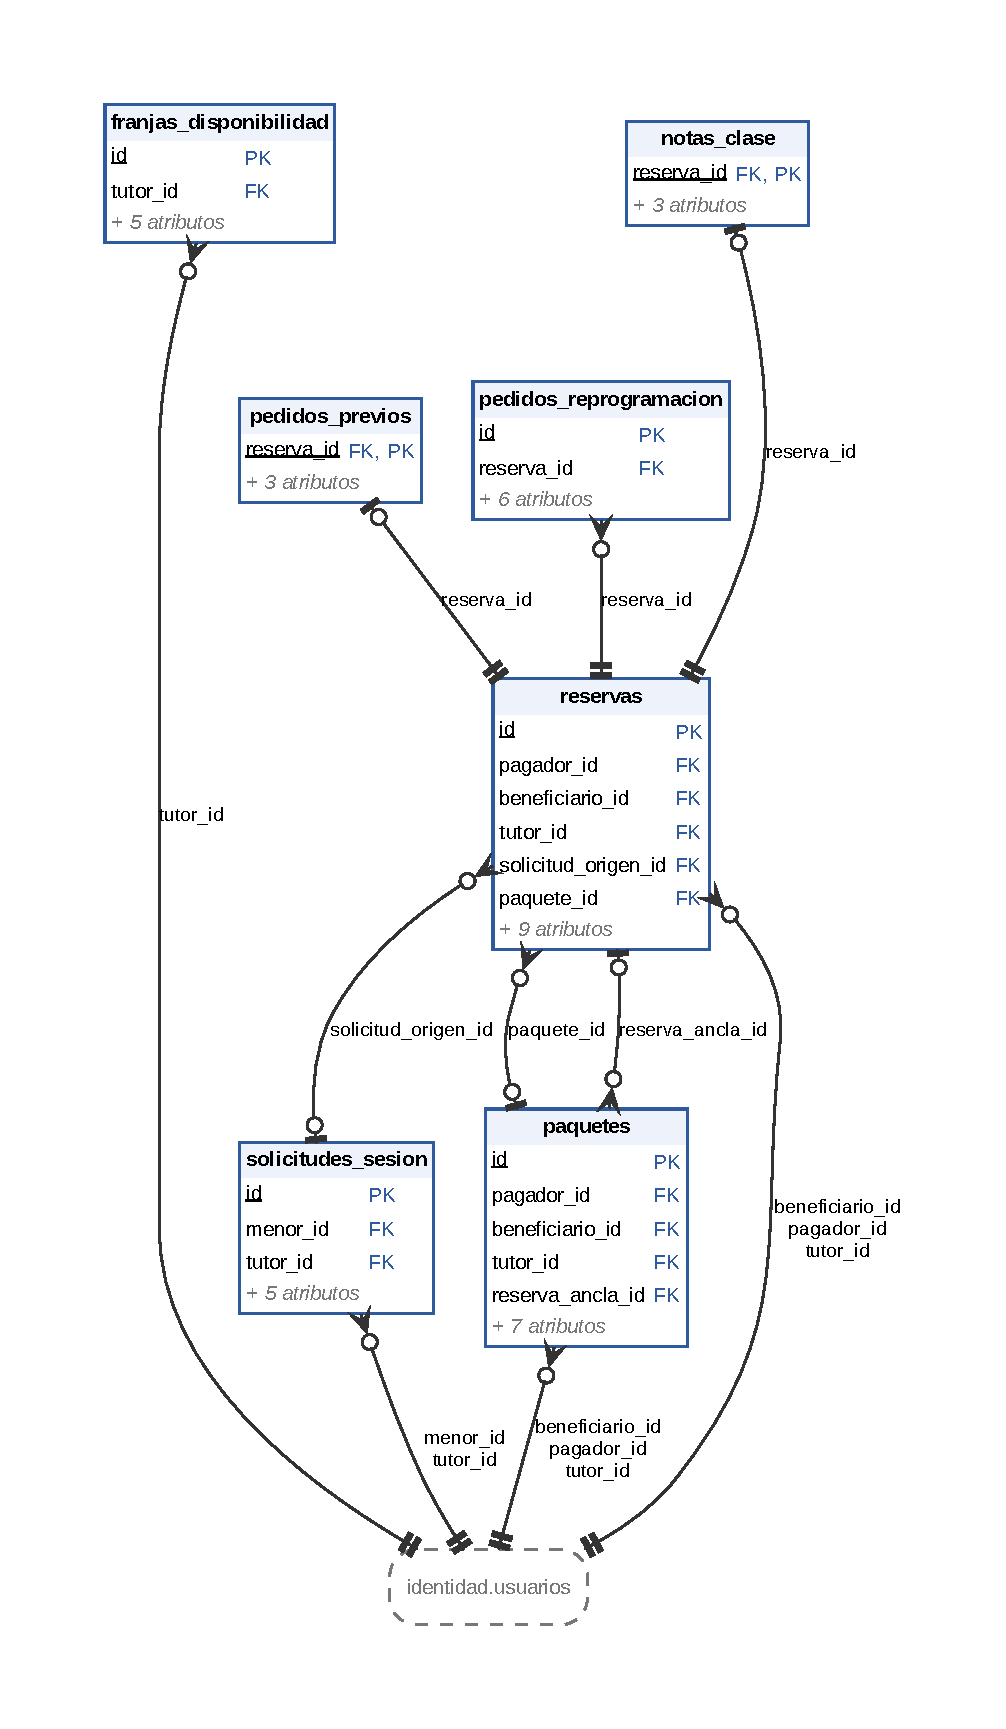
\includegraphics[scale=0.747]{figuras/der/reservas}
    \caption{Diagrama entidad-relación del esquema \texttt{reservas} (M4)}
    \label{fig:der-reservas}
\end{figure}

\subsubsection{\texorpdfstring{\texttt{reservas.franjas\_\allowbreak{}disponibilidad}}{reservas.franjas\_disponibilidad}}\label{dd:reservas.franjas_disponibilidad}

Franjas que publica el tutor: semanales (día de la semana) o puntuales (fecha). Solo se reserva dentro de una franja activa. \emph{Migraciones:} V9, V29, V34.

{\small
\begin{xltabular}{\textwidth}{@{}>{\raggedright\arraybackslash}p{3.6cm} >{\raggedright\arraybackslash}p{2.3cm} >{\raggedright\arraybackslash}p{1cm} >{\centering\arraybackslash}p{0.85cm} L@{}}
    \toprule
    \tb{Atributo} & \tb{Tipo} & \tb{Clave} & \tb{Nulo} & \tb{Descripción} \\
    \midrule
    \endfirsthead
    \toprule
    \tb{Atributo} & \tb{Tipo} & \tb{Clave} & \tb{Nulo} & \tb{Descripción} \\
    \midrule
    \endhead
    \bottomrule
    \endfoot
    \texttt{id} & \texttt{uuid} & PK & no & Identificador (UUID generado por la base) \\
    \texttt{tutor\_\allowbreak{}id} & \texttt{uuid} & FK & no & Tutor que publica la franja \\
    \texttt{dia\_\allowbreak{}semana} & \texttt{smallint} &  & sí & Día de la semana de una franja semanal (0 = domingo a 6 = sábado) \\
    \texttt{fecha\_\allowbreak{}especifica} & \texttt{date} &  & sí & Fecha de una franja puntual \\
    \texttt{hora\_\allowbreak{}inicio} & \texttt{time} &  & no & Hora de inicio (hora de Argentina) \\
    \texttt{hora\_\allowbreak{}fin} & \texttt{time} &  & no & Hora de fin, posterior al inicio \\
    \texttt{activa} & \texttt{boolean} &  & no & La franja está publicada. Por defecto: \texttt{true} \\
\end{xltabular}
}

{\small
\begin{xltabular}{\textwidth}{@{}>{\raggedright\arraybackslash}p{1.7cm} >{\raggedright\arraybackslash}p{4.6cm} L@{}}
    \toprule
    \tb{Tipo} & \tb{Nombre} & \tb{Definición} \\
    \midrule
    \endfirsthead
    \toprule
    \tb{Tipo} & \tb{Nombre} & \tb{Definición} \\
    \midrule
    \endhead
    \bottomrule
    \endfoot
    CHECK & \texttt{chk\_\allowbreak{}franja\_\allowbreak{}modo} & \texttt{(\allowbreak{}(\allowbreak{}dia\_\allowbreak{}semana IS NOT NULL) AND (\allowbreak{}fecha\_\allowbreak{}especifica IS NULL)) OR (\allowbreak{}(\allowbreak{}dia\_\allowbreak{}semana IS NULL) AND (\allowbreak{}fecha\_\allowbreak{}especifica IS NOT NULL))} \\
    CHECK & \texttt{franjas\_\allowbreak{}disponibilidad\_\allowbreak{}check} & \texttt{hora\_\allowbreak{}fin \textgreater{} hora\_\allowbreak{}inicio} \\
    CHECK & \texttt{franjas\_\allowbreak{}disponibilidad\_\allowbreak{}dia\_\allowbreak{}semana\_\allowbreak{}check} & \texttt{(\allowbreak{}dia\_\allowbreak{}semana \textgreater{}= 0) AND (\allowbreak{}dia\_\allowbreak{}semana \textless{}= 6)} \\
    FK & \texttt{franjas\_\allowbreak{}disponibilidad\_\allowbreak{}tutor\_\allowbreak{}id\_\allowbreak{}fkey} & \texttt{(\allowbreak{}tutor\_\allowbreak{}id) $\rightarrow$ identidad.usuarios(\allowbreak{}id)} \\
    PK & \texttt{franjas\_\allowbreak{}disponibilidad\_\allowbreak{}pkey} & \texttt{(\allowbreak{}id)} \\
    EXCLUDE & \texttt{ex\_\allowbreak{}franjas\_\allowbreak{}puntual\_\allowbreak{}sin\_\allowbreak{}superposicion} & \texttt{gist (\allowbreak{}tutor\_\allowbreak{}id WITH =,\allowbreak{} fecha\_\allowbreak{}especifica WITH =,\allowbreak{} tsrange(\allowbreak{}(\allowbreak{}fecha\_\allowbreak{}especifica + hora\_\allowbreak{}inicio),\allowbreak{} (\allowbreak{}fecha\_\allowbreak{}especifica + hora\_\allowbreak{}fin),\allowbreak{} \textquotesingle{}[)\textquotesingle{}) WITH \&\&) WHERE (\allowbreak{}activa AND (\allowbreak{}fecha\_\allowbreak{}especifica IS NOT NULL))} \\
    EXCLUDE & \texttt{ex\_\allowbreak{}franjas\_\allowbreak{}semanal\_\allowbreak{}sin\_\allowbreak{}superposicion} & \texttt{gist (\allowbreak{}tutor\_\allowbreak{}id WITH =,\allowbreak{} dia\_\allowbreak{}semana WITH =,\allowbreak{} tsrange(\allowbreak{}(\allowbreak{}\textquotesingle{}2000-01-01\textquotesingle{}::date + hora\_\allowbreak{}inicio),\allowbreak{} (\allowbreak{}\textquotesingle{}2000-01-01\textquotesingle{}::date + hora\_\allowbreak{}fin),\allowbreak{} \textquotesingle{}[)\textquotesingle{}) WITH \&\&) WHERE (\allowbreak{}activa AND (\allowbreak{}dia\_\allowbreak{}semana IS NOT NULL))} \\
    Índice & \texttt{idx\_\allowbreak{}franjas\_\allowbreak{}tutor\_\allowbreak{}activa} & \texttt{(\allowbreak{}tutor\_\allowbreak{}id,\allowbreak{} activa)} \\
\end{xltabular}
}

\subsubsection{\texorpdfstring{\texttt{reservas.notas\_\allowbreak{}clase}}{reservas.notas\_clase}}\label{dd:reservas.notas_clase}

Nota del tutor al Adulto Responsable sobre la clase (una fila por reserva). \emph{Migraciones:} V44.

{\small
\begin{xltabular}{\textwidth}{@{}>{\raggedright\arraybackslash}p{3.6cm} >{\raggedright\arraybackslash}p{2.3cm} >{\raggedright\arraybackslash}p{1cm} >{\centering\arraybackslash}p{0.85cm} L@{}}
    \toprule
    \tb{Atributo} & \tb{Tipo} & \tb{Clave} & \tb{Nulo} & \tb{Descripción} \\
    \midrule
    \endfirsthead
    \toprule
    \tb{Atributo} & \tb{Tipo} & \tb{Clave} & \tb{Nulo} & \tb{Descripción} \\
    \midrule
    \endhead
    \bottomrule
    \endfoot
    \texttt{reserva\_\allowbreak{}id} & \texttt{uuid} & FK, PK & no & Reserva a la que corresponde la nota \\
    \texttt{texto} & \texttt{varchar(\allowbreak{}1000)} &  & no & Contenido de la nota (hasta 1000 caracteres) \\
    \texttt{created\_\allowbreak{}at} & \texttt{timestamptz} &  & no & Fecha y hora de creación de la fila. Por defecto: \texttt{now(\allowbreak{})} \\
    \texttt{updated\_\allowbreak{}at} & \texttt{timestamptz} &  & no & Fecha y hora de la última edición. Por defecto: \texttt{now(\allowbreak{})} \\
\end{xltabular}
}

{\small
\begin{xltabular}{\textwidth}{@{}>{\raggedright\arraybackslash}p{1.7cm} >{\raggedright\arraybackslash}p{4.6cm} L@{}}
    \toprule
    \tb{Tipo} & \tb{Nombre} & \tb{Definición} \\
    \midrule
    \endfirsthead
    \toprule
    \tb{Tipo} & \tb{Nombre} & \tb{Definición} \\
    \midrule
    \endhead
    \bottomrule
    \endfoot
    FK & \texttt{notas\_\allowbreak{}clase\_\allowbreak{}reserva\_\allowbreak{}id\_\allowbreak{}fkey} & \texttt{(\allowbreak{}reserva\_\allowbreak{}id) $\rightarrow$ reservas.reservas(\allowbreak{}id)} \\
    PK & \texttt{notas\_\allowbreak{}clase\_\allowbreak{}pkey} & \texttt{(\allowbreak{}reserva\_\allowbreak{}id)} \\
\end{xltabular}
}

\subsubsection{\texorpdfstring{\texttt{reservas.paquetes}}{reservas.paquetes}}\label{dd:reservas.paquetes}

Paquete mensual: varias clases semanales con un solo pago (ADR-M5-03). Cada clase es una reserva con \path{paquete_id}; la primera es el ancla del pago. \emph{Migraciones:} V46.

{\small
\begin{xltabular}{\textwidth}{@{}>{\raggedright\arraybackslash}p{3.6cm} >{\raggedright\arraybackslash}p{2.3cm} >{\raggedright\arraybackslash}p{1cm} >{\centering\arraybackslash}p{0.85cm} L@{}}
    \toprule
    \tb{Atributo} & \tb{Tipo} & \tb{Clave} & \tb{Nulo} & \tb{Descripción} \\
    \midrule
    \endfirsthead
    \toprule
    \tb{Atributo} & \tb{Tipo} & \tb{Clave} & \tb{Nulo} & \tb{Descripción} \\
    \midrule
    \endhead
    \bottomrule
    \endfoot
    \texttt{id} & \texttt{uuid} & PK & no & Identificador (UUID generado por la aplicación) \\
    \texttt{pagador\_\allowbreak{}id} & \texttt{uuid} & FK & no & Quien paga el paquete \\
    \texttt{beneficiario\_\allowbreak{}id} & \texttt{uuid} & FK & no & Quien recibe las clases \\
    \texttt{tutor\_\allowbreak{}id} & \texttt{uuid} & FK & no & Tutor que dicta las clases \\
    \texttt{reserva\_\allowbreak{}ancla\_\allowbreak{}id} & \texttt{uuid} & FK & sí & Primera reserva del paquete; es la referencia del pago en MercadoPago \\
    \texttt{cantidad\_\allowbreak{}clases} & \texttt{integer} &  & no & Cantidad de clases del paquete \\
    \texttt{duracion\_\allowbreak{}minutos} & \texttt{integer} &  & no & Duración de cada clase \\
    \texttt{descuento\_\allowbreak{}porcentaje} & \texttt{integer} &  & no & Descuento aplicado (0 a 30\,\%) \\
    \texttt{precio\_\allowbreak{}total} & \texttt{numeric(\allowbreak{}10,\allowbreak{}2)} &  & no & Precio total congelado del paquete \\
    \texttt{estado} & \texttt{varchar(\allowbreak{}20)} &  & no & pendiente\_pago, confirmado o cancelado \\
    \texttt{vigente\_\allowbreak{}hasta} & \texttt{timestamptz} &  & no & Fin de la vigencia del paquete \\
    \texttt{created\_\allowbreak{}at} & \texttt{timestamptz} &  & no & Fecha y hora de creación de la fila. Por defecto: \texttt{now(\allowbreak{})} \\
\end{xltabular}
}

{\small
\begin{xltabular}{\textwidth}{@{}>{\raggedright\arraybackslash}p{1.7cm} >{\raggedright\arraybackslash}p{4.6cm} L@{}}
    \toprule
    \tb{Tipo} & \tb{Nombre} & \tb{Definición} \\
    \midrule
    \endfirsthead
    \toprule
    \tb{Tipo} & \tb{Nombre} & \tb{Definición} \\
    \midrule
    \endhead
    \bottomrule
    \endfoot
    CHECK & \texttt{paquetes\_\allowbreak{}cantidad\_\allowbreak{}clases\_\allowbreak{}check} & \texttt{cantidad\_\allowbreak{}clases \textgreater{} 0} \\
    CHECK & \texttt{paquetes\_\allowbreak{}descuento\_\allowbreak{}porcentaje\_\allowbreak{}check} & \texttt{(\allowbreak{}descuento\_\allowbreak{}porcentaje \textgreater{}= 0) AND (\allowbreak{}descuento\_\allowbreak{}porcentaje \textless{}= 30)} \\
    CHECK & \texttt{paquetes\_\allowbreak{}estado\_\allowbreak{}check} & \texttt{estado IN (\allowbreak{}\textquotesingle{}pendiente\_\allowbreak{}pago\textquotesingle{},\allowbreak{} \textquotesingle{}confirmado\textquotesingle{},\allowbreak{} \textquotesingle{}cancelado\textquotesingle{})} \\
    CHECK & \texttt{paquetes\_\allowbreak{}precio\_\allowbreak{}total\_\allowbreak{}check} & \texttt{precio\_\allowbreak{}total \textgreater{}= 0} \\
    FK & \texttt{fk\_\allowbreak{}paquetes\_\allowbreak{}reserva\_\allowbreak{}ancla} & \texttt{(\allowbreak{}reserva\_\allowbreak{}ancla\_\allowbreak{}id) $\rightarrow$ reservas.reservas(\allowbreak{}id)} \\
    FK & \texttt{paquetes\_\allowbreak{}beneficiario\_\allowbreak{}id\_\allowbreak{}fkey} & \texttt{(\allowbreak{}beneficiario\_\allowbreak{}id) $\rightarrow$ identidad.usuarios(\allowbreak{}id)} \\
    FK & \texttt{paquetes\_\allowbreak{}pagador\_\allowbreak{}id\_\allowbreak{}fkey} & \texttt{(\allowbreak{}pagador\_\allowbreak{}id) $\rightarrow$ identidad.usuarios(\allowbreak{}id)} \\
    FK & \texttt{paquetes\_\allowbreak{}tutor\_\allowbreak{}id\_\allowbreak{}fkey} & \texttt{(\allowbreak{}tutor\_\allowbreak{}id) $\rightarrow$ identidad.usuarios(\allowbreak{}id)} \\
    PK & \texttt{paquetes\_\allowbreak{}pkey} & \texttt{(\allowbreak{}id)} \\
\end{xltabular}
}

\subsubsection{\texorpdfstring{\texttt{reservas.pedidos\_\allowbreak{}previos}}{reservas.pedidos\_previos}}\label{dd:reservas.pedidos_previos}

Texto que el alumno o su Adulto Responsable deja antes de la clase para el tutor (una fila por reserva). \emph{Migraciones:} V44.

{\small
\begin{xltabular}{\textwidth}{@{}>{\raggedright\arraybackslash}p{3.6cm} >{\raggedright\arraybackslash}p{2.3cm} >{\raggedright\arraybackslash}p{1cm} >{\centering\arraybackslash}p{0.85cm} L@{}}
    \toprule
    \tb{Atributo} & \tb{Tipo} & \tb{Clave} & \tb{Nulo} & \tb{Descripción} \\
    \midrule
    \endfirsthead
    \toprule
    \tb{Atributo} & \tb{Tipo} & \tb{Clave} & \tb{Nulo} & \tb{Descripción} \\
    \midrule
    \endhead
    \bottomrule
    \endfoot
    \texttt{reserva\_\allowbreak{}id} & \texttt{uuid} & FK, PK & no & Reserva a la que corresponde el pedido \\
    \texttt{texto} & \texttt{varchar(\allowbreak{}1000)} &  & no & Contenido del pedido (hasta 1000 caracteres) \\
    \texttt{created\_\allowbreak{}at} & \texttt{timestamptz} &  & no & Fecha y hora de creación de la fila. Por defecto: \texttt{now(\allowbreak{})} \\
    \texttt{updated\_\allowbreak{}at} & \texttt{timestamptz} &  & no & Fecha y hora de la última edición. Por defecto: \texttt{now(\allowbreak{})} \\
\end{xltabular}
}

{\small
\begin{xltabular}{\textwidth}{@{}>{\raggedright\arraybackslash}p{1.7cm} >{\raggedright\arraybackslash}p{4.6cm} L@{}}
    \toprule
    \tb{Tipo} & \tb{Nombre} & \tb{Definición} \\
    \midrule
    \endfirsthead
    \toprule
    \tb{Tipo} & \tb{Nombre} & \tb{Definición} \\
    \midrule
    \endhead
    \bottomrule
    \endfoot
    FK & \texttt{pedidos\_\allowbreak{}previos\_\allowbreak{}reserva\_\allowbreak{}id\_\allowbreak{}fkey} & \texttt{(\allowbreak{}reserva\_\allowbreak{}id) $\rightarrow$ reservas.reservas(\allowbreak{}id)} \\
    PK & \texttt{pedidos\_\allowbreak{}previos\_\allowbreak{}pkey} & \texttt{(\allowbreak{}reserva\_\allowbreak{}id)} \\
\end{xltabular}
}

\subsubsection{\texorpdfstring{\texttt{reservas.pedidos\_\allowbreak{}reprogramacion}}{reservas.pedidos\_reprogramacion}}\label{dd:reservas.pedidos_reprogramacion}

Pedido del tutor para cambiar el horario de una reserva. Puede haber uno solo pendiente por reserva; los resueltos quedan como historial. \emph{Migraciones:} V45.

{\small
\begin{xltabular}{\textwidth}{@{}>{\raggedright\arraybackslash}p{3.6cm} >{\raggedright\arraybackslash}p{2.3cm} >{\raggedright\arraybackslash}p{1cm} >{\centering\arraybackslash}p{0.85cm} L@{}}
    \toprule
    \tb{Atributo} & \tb{Tipo} & \tb{Clave} & \tb{Nulo} & \tb{Descripción} \\
    \midrule
    \endfirsthead
    \toprule
    \tb{Atributo} & \tb{Tipo} & \tb{Clave} & \tb{Nulo} & \tb{Descripción} \\
    \midrule
    \endhead
    \bottomrule
    \endfoot
    \texttt{id} & \texttt{uuid} & PK & no & Identificador (UUID generado por la aplicación) \\
    \texttt{reserva\_\allowbreak{}id} & \texttt{uuid} & FK & no & Reserva que se quiere reprogramar \\
    \texttt{horario\_\allowbreak{}original} & \texttt{timestamptz} &  & no & Horario de la reserva al hacer el pedido \\
    \texttt{horario\_\allowbreak{}propuesto} & \texttt{timestamptz} &  & no & Nuevo horario propuesto \\
    \texttt{motivo} & \texttt{varchar(\allowbreak{}300)} &  & sí & Motivo informado por el tutor \\
    \texttt{estado} & \texttt{varchar(\allowbreak{}20)} &  & no & pendiente, aceptado, rechazado, vencido o retirado \\
    \texttt{created\_\allowbreak{}at} & \texttt{timestamptz} &  & no & Fecha y hora de creación de la fila. Por defecto: \texttt{now(\allowbreak{})} \\
    \texttt{resuelto\_\allowbreak{}at} & \texttt{timestamptz} &  & sí & Fecha y hora de la resolución \\
\end{xltabular}
}

{\small
\begin{xltabular}{\textwidth}{@{}>{\raggedright\arraybackslash}p{1.7cm} >{\raggedright\arraybackslash}p{4.6cm} L@{}}
    \toprule
    \tb{Tipo} & \tb{Nombre} & \tb{Definición} \\
    \midrule
    \endfirsthead
    \toprule
    \tb{Tipo} & \tb{Nombre} & \tb{Definición} \\
    \midrule
    \endhead
    \bottomrule
    \endfoot
    CHECK & \texttt{pedidos\_\allowbreak{}reprogramacion\_\allowbreak{}estado\_\allowbreak{}check} & \texttt{estado IN (\allowbreak{}\textquotesingle{}pendiente\textquotesingle{},\allowbreak{} \textquotesingle{}aceptado\textquotesingle{},\allowbreak{} \textquotesingle{}rechazado\textquotesingle{},\allowbreak{} \textquotesingle{}vencido\textquotesingle{},\allowbreak{} \textquotesingle{}retirado\textquotesingle{})} \\
    FK & \texttt{pedidos\_\allowbreak{}reprogramacion\_\allowbreak{}reserva\_\allowbreak{}id\_\allowbreak{}fkey} & \texttt{(\allowbreak{}reserva\_\allowbreak{}id) $\rightarrow$ reservas.reservas(\allowbreak{}id)} \\
    PK & \texttt{pedidos\_\allowbreak{}reprogramacion\_\allowbreak{}pkey} & \texttt{(\allowbreak{}id)} \\
    UNIQUE & \texttt{uq\_\allowbreak{}pedido\_\allowbreak{}reprogramacion\_\allowbreak{}pendiente} & \texttt{(\allowbreak{}reserva\_\allowbreak{}id) WHERE estado = \textquotesingle{}pendiente\textquotesingle{}} \\
\end{xltabular}
}

\subsubsection{\texorpdfstring{\texttt{reservas.reservas}}{reservas.reservas}}\label{dd:reservas.reservas}

Clase reservada. Distingue a quien paga, a quien recibe la clase y al tutor, y congela el precio y la duración al crearse. \emph{Migraciones:} V9, V11, V29, V30, V35, V36, V37, V38, V44, V45, V46.

{\small
\begin{xltabular}{\textwidth}{@{}>{\raggedright\arraybackslash}p{3.6cm} >{\raggedright\arraybackslash}p{2.3cm} >{\raggedright\arraybackslash}p{1cm} >{\centering\arraybackslash}p{0.85cm} L@{}}
    \toprule
    \tb{Atributo} & \tb{Tipo} & \tb{Clave} & \tb{Nulo} & \tb{Descripción} \\
    \midrule
    \endfirsthead
    \toprule
    \tb{Atributo} & \tb{Tipo} & \tb{Clave} & \tb{Nulo} & \tb{Descripción} \\
    \midrule
    \endhead
    \bottomrule
    \endfoot
    \texttt{id} & \texttt{uuid} & PK & no & Identificador (UUID generado por la base) \\
    \texttt{pagador\_\allowbreak{}id} & \texttt{uuid} & FK & no & Quien paga: el estudiante adulto o el Adulto Responsable \\
    \texttt{beneficiario\_\allowbreak{}id} & \texttt{uuid} & FK & no & Quien recibe la clase \\
    \texttt{tutor\_\allowbreak{}id} & \texttt{uuid} & FK & no & Tutor que dicta la clase \\
    \texttt{solicitud\_\allowbreak{}origen\_\allowbreak{}id} & \texttt{uuid} & FK & sí & Solicitud del menor que originó la reserva, si la hubo \\
    \texttt{horario} & \texttt{timestamptz} &  & no & Inicio de la clase \\
    \texttt{precio} & \texttt{numeric(\allowbreak{}10,\allowbreak{}2)} &  & no & Precio de la clase, congelado al reservar \\
    \texttt{estado} & \texttt{varchar(\allowbreak{}20)} &  & no & Estado de la reserva. Por defecto: \texttt{\textquotesingle{}pendiente\_\allowbreak{}pago\textquotesingle{}} \\
    \texttt{motivo\_\allowbreak{}cancelacion} & \texttt{varchar(\allowbreak{}30)} &  & sí & Motivo de la cancelación; obligatorio solo en estado \texttt{cancelada} \\
    \texttt{created\_\allowbreak{}at} & \texttt{timestamptz} &  & no & Fecha y hora de creación de la fila. Por defecto: \texttt{now(\allowbreak{})} \\
    \texttt{duracion\_\allowbreak{}minutos} & \texttt{integer} &  & no & Duración (30 a 180 minutos, en bloques de 30) \\
    \texttt{horario\_\allowbreak{}fin} & \texttt{timestamptz} &  & no & Fin de la clase; existe porque una restricción EXCLUDE no admite \texttt{horario + intervalo} \\
    \texttt{resumen\_\allowbreak{}contratado} & \texttt{boolean} &  & no & Se contrató el adicional de resumen. Por defecto: \texttt{false} \\
    \texttt{precio\_\allowbreak{}adicional\_\allowbreak{}resumen} & \texttt{numeric(\allowbreak{}10,\allowbreak{}2)} &  & sí & Precio congelado del adicional; presente si y solo si se contrató \\
    \texttt{paquete\_\allowbreak{}id} & \texttt{uuid} & FK & sí & Paquete mensual al que pertenece la clase, si lo hay \\
\end{xltabular}
}

{\small
\begin{xltabular}{\textwidth}{@{}>{\raggedright\arraybackslash}p{1.7cm} >{\raggedright\arraybackslash}p{4.6cm} L@{}}
    \toprule
    \tb{Tipo} & \tb{Nombre} & \tb{Definición} \\
    \midrule
    \endfirsthead
    \toprule
    \tb{Tipo} & \tb{Nombre} & \tb{Definición} \\
    \midrule
    \endhead
    \bottomrule
    \endfoot
    CHECK & \texttt{chk\_\allowbreak{}motivo\_\allowbreak{}solo\_\allowbreak{}si\_\allowbreak{}cancelada} & \texttt{(\allowbreak{}(\allowbreak{}estado = \textquotesingle{}cancelada\textquotesingle{}) AND (\allowbreak{}motivo\_\allowbreak{}cancelacion IS NOT NULL)) OR (\allowbreak{}(\allowbreak{}estado \textless{}\textgreater{} \textquotesingle{}cancelada\textquotesingle{}) AND (\allowbreak{}motivo\_\allowbreak{}cancelacion IS NULL))} \\
    CHECK & \texttt{chk\_\allowbreak{}reservas\_\allowbreak{}duracion} & \texttt{(\allowbreak{}(\allowbreak{}duracion\_\allowbreak{}minutos \textgreater{}= 30) AND (\allowbreak{}duracion\_\allowbreak{}minutos \textless{}= 180)) AND (\allowbreak{}(\allowbreak{}duracion\_\allowbreak{}minutos \% 30) = 0)} \\
    CHECK & \texttt{chk\_\allowbreak{}reservas\_\allowbreak{}fin\_\allowbreak{}posterior} & \texttt{horario\_\allowbreak{}fin \textgreater{} horario} \\
    CHECK & \texttt{ck\_\allowbreak{}reservas\_\allowbreak{}tutor\_\allowbreak{}no\_\allowbreak{}es\_\allowbreak{}parte} & \texttt{(\allowbreak{}tutor\_\allowbreak{}id \textless{}\textgreater{} pagador\_\allowbreak{}id) AND (\allowbreak{}tutor\_\allowbreak{}id \textless{}\textgreater{} beneficiario\_\allowbreak{}id)} \\
    CHECK & \texttt{reservas\_\allowbreak{}adicional\_\allowbreak{}resumen\_\allowbreak{}check} & \texttt{resumen\_\allowbreak{}contratado = (\allowbreak{}precio\_\allowbreak{}adicional\_\allowbreak{}resumen IS NOT NULL)} \\
    CHECK & \texttt{reservas\_\allowbreak{}estado\_\allowbreak{}check} & \texttt{estado IN (\allowbreak{}\textquotesingle{}pendiente\_\allowbreak{}pago\textquotesingle{},\allowbreak{} \textquotesingle{}confirmada\textquotesingle{},\allowbreak{} \textquotesingle{}en\_\allowbreak{}curso\textquotesingle{},\allowbreak{} \textquotesingle{}finalizada\textquotesingle{},\allowbreak{} \textquotesingle{}cancelada\textquotesingle{},\allowbreak{} \textquotesingle{}no\_\allowbreak{}show\_\allowbreak{}estudiante\textquotesingle{},\allowbreak{} \textquotesingle{}no\_\allowbreak{}show\_\allowbreak{}tutor\textquotesingle{},\allowbreak{} \textquotesingle{}no\_\allowbreak{}show\_\allowbreak{}doble\textquotesingle{})} \\
    CHECK & \texttt{reservas\_\allowbreak{}motivo\_\allowbreak{}cancelacion\_\allowbreak{}check} & \texttt{motivo\_\allowbreak{}cancelacion IN (\allowbreak{}\textquotesingle{}voluntaria\textquotesingle{},\allowbreak{} \textquotesingle{}timeout\_\allowbreak{}pago\textquotesingle{},\allowbreak{} \textquotesingle{}revocacion\_\allowbreak{}autorizacion\textquotesingle{},\allowbreak{} \textquotesingle{}sancion\textquotesingle{},\allowbreak{} \textquotesingle{}cap\_\allowbreak{}vencido\textquotesingle{})} \\
    CHECK & \texttt{reservas\_\allowbreak{}precio\_\allowbreak{}check} & \texttt{precio \textgreater{}= 0} \\
    FK & \texttt{reservas\_\allowbreak{}beneficiario\_\allowbreak{}id\_\allowbreak{}fkey} & \texttt{(\allowbreak{}beneficiario\_\allowbreak{}id) $\rightarrow$ identidad.usuarios(\allowbreak{}id)} \\
    FK & \texttt{reservas\_\allowbreak{}pagador\_\allowbreak{}id\_\allowbreak{}fkey} & \texttt{(\allowbreak{}pagador\_\allowbreak{}id) $\rightarrow$ identidad.usuarios(\allowbreak{}id)} \\
    FK & \texttt{reservas\_\allowbreak{}paquete\_\allowbreak{}id\_\allowbreak{}fkey} & \texttt{(\allowbreak{}paquete\_\allowbreak{}id) $\rightarrow$ reservas.paquetes(\allowbreak{}id)} \\
    FK & \texttt{reservas\_\allowbreak{}solicitud\_\allowbreak{}origen\_\allowbreak{}id\_\allowbreak{}fkey} & \texttt{(\allowbreak{}solicitud\_\allowbreak{}origen\_\allowbreak{}id) $\rightarrow$ reservas.solicitudes\_\allowbreak{}sesion(\allowbreak{}id)} \\
    FK & \texttt{reservas\_\allowbreak{}tutor\_\allowbreak{}id\_\allowbreak{}fkey} & \texttt{(\allowbreak{}tutor\_\allowbreak{}id) $\rightarrow$ identidad.usuarios(\allowbreak{}id)} \\
    PK & \texttt{reservas\_\allowbreak{}pkey} & \texttt{(\allowbreak{}id)} \\
    EXCLUDE & \texttt{ex\_\allowbreak{}reservas\_\allowbreak{}rango\_\allowbreak{}beneficiario} & \texttt{gist (\allowbreak{}beneficiario\_\allowbreak{}id WITH =,\allowbreak{} tstzrange(\allowbreak{}horario,\allowbreak{} horario\_\allowbreak{}fin,\allowbreak{} \textquotesingle{}[)\textquotesingle{}) WITH \&\&) WHERE (\allowbreak{}estado \textless{}\textgreater{} \textquotesingle{}cancelada\textquotesingle{})} \\
    EXCLUDE & \texttt{ex\_\allowbreak{}reservas\_\allowbreak{}rango\_\allowbreak{}tutor} & \texttt{gist (\allowbreak{}tutor\_\allowbreak{}id WITH =,\allowbreak{} tstzrange(\allowbreak{}horario,\allowbreak{} horario\_\allowbreak{}fin,\allowbreak{} \textquotesingle{}[)\textquotesingle{}) WITH \&\&) WHERE (\allowbreak{}estado \textless{}\textgreater{} \textquotesingle{}cancelada\textquotesingle{})} \\
    Índice & \texttt{idx\_\allowbreak{}reservas\_\allowbreak{}beneficiario\_\allowbreak{}horario} & \texttt{(\allowbreak{}beneficiario\_\allowbreak{}id,\allowbreak{} horario)} \\
    Índice & \texttt{idx\_\allowbreak{}reservas\_\allowbreak{}paquete} & \texttt{(\allowbreak{}paquete\_\allowbreak{}id) WHERE paquete\_\allowbreak{}id IS NOT NULL} \\
    Índice & \texttt{idx\_\allowbreak{}reservas\_\allowbreak{}tutor\_\allowbreak{}horario} & \texttt{(\allowbreak{}tutor\_\allowbreak{}id,\allowbreak{} horario)} \\
\end{xltabular}
}

\subsubsection{\texorpdfstring{\texttt{reservas.solicitudes\_\allowbreak{}sesion}}{reservas.solicitudes\_sesion}}\label{dd:reservas.solicitudes_sesion}

Pedido de clase que hace un menor. No bloquea el horario ni genera cobro: el Adulto Responsable la aprueba y paga para convertirla en reserva. Vence a las 48 horas. \emph{Migraciones:} V9, V29.

{\small
\begin{xltabular}{\textwidth}{@{}>{\raggedright\arraybackslash}p{3.6cm} >{\raggedright\arraybackslash}p{2.3cm} >{\raggedright\arraybackslash}p{1cm} >{\centering\arraybackslash}p{0.85cm} L@{}}
    \toprule
    \tb{Atributo} & \tb{Tipo} & \tb{Clave} & \tb{Nulo} & \tb{Descripción} \\
    \midrule
    \endfirsthead
    \toprule
    \tb{Atributo} & \tb{Tipo} & \tb{Clave} & \tb{Nulo} & \tb{Descripción} \\
    \midrule
    \endhead
    \bottomrule
    \endfoot
    \texttt{id} & \texttt{uuid} & PK & no & Identificador (UUID generado por la base) \\
    \texttt{menor\_\allowbreak{}id} & \texttt{uuid} & FK & no & Menor que pide la clase \\
    \texttt{tutor\_\allowbreak{}id} & \texttt{uuid} & FK & no & Tutor pedido \\
    \texttt{horario\_\allowbreak{}propuesto} & \texttt{timestamptz} &  & no & Inicio propuesto para la clase \\
    \texttt{estado} & \texttt{varchar(\allowbreak{}20)} &  & no & pendiente, convertida, expirada o rechazada. Por defecto: \texttt{\textquotesingle{}pendiente\textquotesingle{}} \\
    \texttt{created\_\allowbreak{}at} & \texttt{timestamptz} &  & no & Fecha y hora de creación de la fila. Por defecto: \texttt{now(\allowbreak{})} \\
    \texttt{expira\_\allowbreak{}at} & \texttt{timestamptz} &  & no & Vencimiento de la solicitud \\
    \texttt{duracion\_\allowbreak{}minutos} & \texttt{integer} &  & no & Duración pedida (30 a 180 minutos, en bloques de 30) \\
\end{xltabular}
}

{\small
\begin{xltabular}{\textwidth}{@{}>{\raggedright\arraybackslash}p{1.7cm} >{\raggedright\arraybackslash}p{4.6cm} L@{}}
    \toprule
    \tb{Tipo} & \tb{Nombre} & \tb{Definición} \\
    \midrule
    \endfirsthead
    \toprule
    \tb{Tipo} & \tb{Nombre} & \tb{Definición} \\
    \midrule
    \endhead
    \bottomrule
    \endfoot
    CHECK & \texttt{chk\_\allowbreak{}solicitudes\_\allowbreak{}duracion} & \texttt{(\allowbreak{}(\allowbreak{}duracion\_\allowbreak{}minutos \textgreater{}= 30) AND (\allowbreak{}duracion\_\allowbreak{}minutos \textless{}= 180)) AND (\allowbreak{}(\allowbreak{}duracion\_\allowbreak{}minutos \% 30) = 0)} \\
    CHECK & \texttt{solicitudes\_\allowbreak{}sesion\_\allowbreak{}check} & \texttt{expira\_\allowbreak{}at \textgreater{} created\_\allowbreak{}at} \\
    CHECK & \texttt{solicitudes\_\allowbreak{}sesion\_\allowbreak{}estado\_\allowbreak{}check} & \texttt{estado IN (\allowbreak{}\textquotesingle{}pendiente\textquotesingle{},\allowbreak{} \textquotesingle{}convertida\textquotesingle{},\allowbreak{} \textquotesingle{}expirada\textquotesingle{},\allowbreak{} \textquotesingle{}rechazada\textquotesingle{})} \\
    FK & \texttt{solicitudes\_\allowbreak{}sesion\_\allowbreak{}menor\_\allowbreak{}id\_\allowbreak{}fkey} & \texttt{(\allowbreak{}menor\_\allowbreak{}id) $\rightarrow$ identidad.usuarios(\allowbreak{}id)} \\
    FK & \texttt{solicitudes\_\allowbreak{}sesion\_\allowbreak{}tutor\_\allowbreak{}id\_\allowbreak{}fkey} & \texttt{(\allowbreak{}tutor\_\allowbreak{}id) $\rightarrow$ identidad.usuarios(\allowbreak{}id)} \\
    PK & \texttt{solicitudes\_\allowbreak{}sesion\_\allowbreak{}pkey} & \texttt{(\allowbreak{}id)} \\
    Índice & \texttt{idx\_\allowbreak{}solicitudes\_\allowbreak{}expiracion} & \texttt{(\allowbreak{}estado,\allowbreak{} expira\_\allowbreak{}at)} \\
    Índice & \texttt{idx\_\allowbreak{}solicitudes\_\allowbreak{}menor\_\allowbreak{}estado} & \texttt{(\allowbreak{}menor\_\allowbreak{}id,\allowbreak{} estado)} \\
\end{xltabular}
}

\subsection{Esquema \texttt{pagos} (M5)}\label{dd:pagos}

Motor de pagos: transacción de cada reserva con su estado de \gls{escrow}, tarifas, cuentas de MercadoPago de los tutores, preferencias de pago y estado global de la pasarela. Tablas: 7. Su diagrama entidad-relación es la figura~\ref{fig:der-pagos}.

\begin{figure}[htbp]
    \centering
    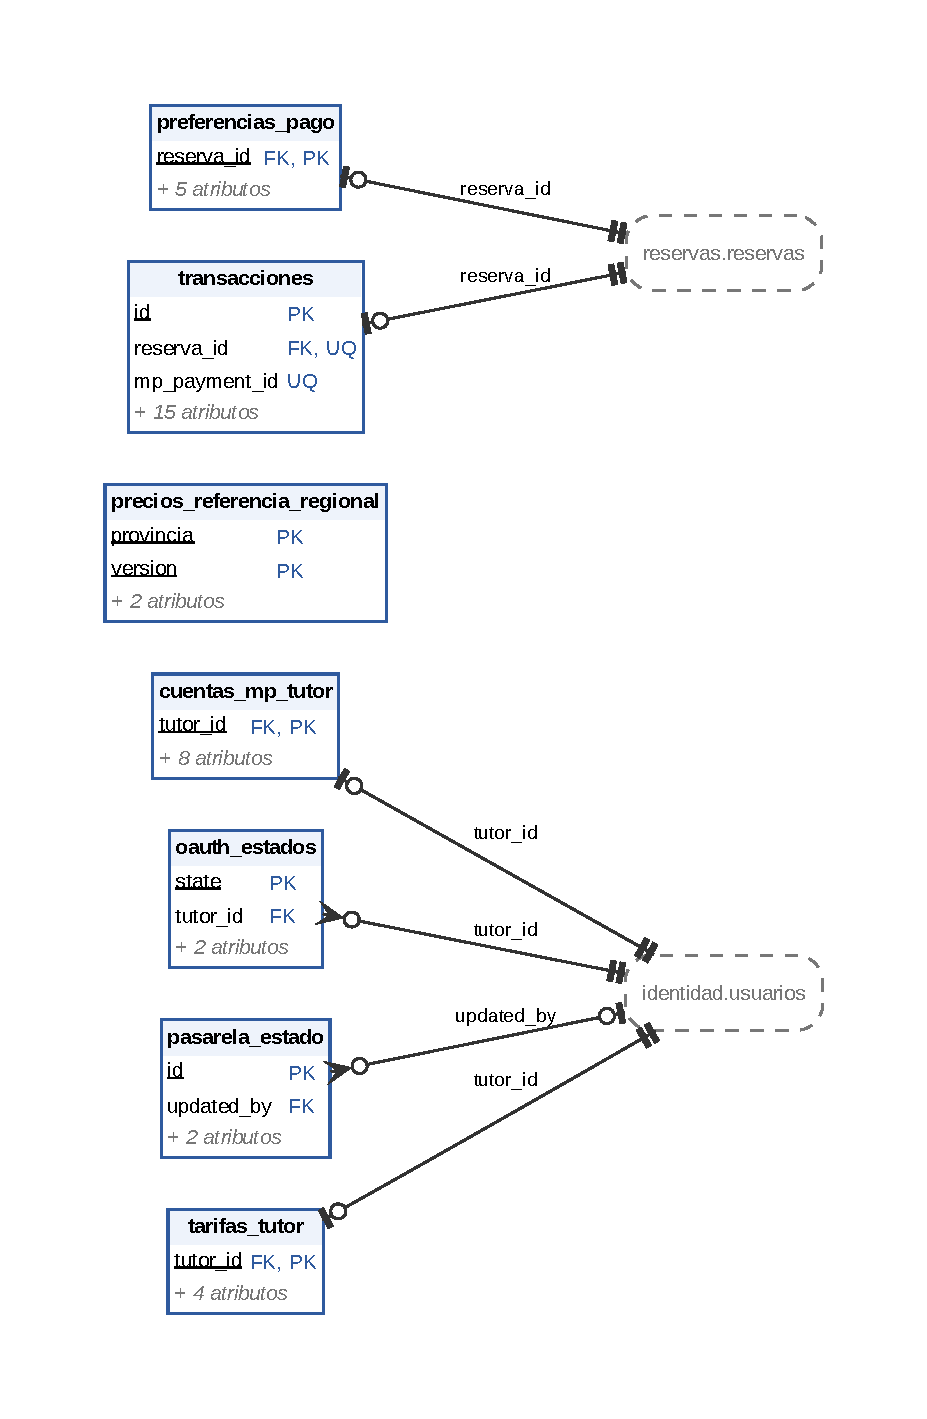
\includegraphics[scale=0.910]{figuras/der/pagos}
    \caption{Diagrama entidad-relación del esquema \texttt{pagos} (M5)}
    \label{fig:der-pagos}
\end{figure}

\subsubsection{\texorpdfstring{\texttt{pagos.cuentas\_\allowbreak{}mp\_\allowbreak{}tutor}}{pagos.cuentas\_mp\_tutor}}\label{dd:pagos.cuentas_mp_tutor}

Cuenta de MercadoPago que cada tutor conecta por \gls{oauth} (modelo A, ADR-M5-02). Los tokens se guardan cifrados con AES-256-GCM y la clave está fuera de la base. \emph{Migraciones:} V39.

{\small
\begin{xltabular}{\textwidth}{@{}>{\raggedright\arraybackslash}p{3.6cm} >{\raggedright\arraybackslash}p{2.3cm} >{\raggedright\arraybackslash}p{1cm} >{\centering\arraybackslash}p{0.85cm} L@{}}
    \toprule
    \tb{Atributo} & \tb{Tipo} & \tb{Clave} & \tb{Nulo} & \tb{Descripción} \\
    \midrule
    \endfirsthead
    \toprule
    \tb{Atributo} & \tb{Tipo} & \tb{Clave} & \tb{Nulo} & \tb{Descripción} \\
    \midrule
    \endhead
    \bottomrule
    \endfoot
    \texttt{tutor\_\allowbreak{}id} & \texttt{uuid} & FK, PK & no & Tutor dueño de la cuenta \\
    \texttt{mp\_\allowbreak{}user\_\allowbreak{}id} & \texttt{varchar(\allowbreak{}40)} &  & no & Identificador del usuario en MercadoPago \\
    \texttt{access\_\allowbreak{}token\_\allowbreak{}cifrado} & \texttt{bytea} &  & no & Token de acceso, cifrado \\
    \texttt{refresh\_\allowbreak{}token\_\allowbreak{}cifrado} & \texttt{bytea} &  & sí & Token de renovación, cifrado \\
    \texttt{public\_\allowbreak{}key} & \texttt{varchar(\allowbreak{}100)} &  & sí & Clave pública de la cuenta \\
    \texttt{expira\_\allowbreak{}at} & \texttt{timestamptz} &  & no & Vencimiento del token de acceso \\
    \texttt{estado} & \texttt{varchar(\allowbreak{}20)} &  & no & CONECTADA, REVOCADA o ERROR \\
    \texttt{conectada\_\allowbreak{}at} & \texttt{timestamptz} &  & no & Fecha y hora de la conexión. Por defecto: \texttt{now(\allowbreak{})} \\
    \texttt{updated\_\allowbreak{}at} & \texttt{timestamptz} &  & no & Fecha y hora de la última modificación. Por defecto: \texttt{now(\allowbreak{})} \\
\end{xltabular}
}

{\small
\begin{xltabular}{\textwidth}{@{}>{\raggedright\arraybackslash}p{1.7cm} >{\raggedright\arraybackslash}p{4.6cm} L@{}}
    \toprule
    \tb{Tipo} & \tb{Nombre} & \tb{Definición} \\
    \midrule
    \endfirsthead
    \toprule
    \tb{Tipo} & \tb{Nombre} & \tb{Definición} \\
    \midrule
    \endhead
    \bottomrule
    \endfoot
    CHECK & \texttt{cuentas\_\allowbreak{}mp\_\allowbreak{}tutor\_\allowbreak{}estado\_\allowbreak{}check} & \texttt{estado IN (\allowbreak{}\textquotesingle{}CONECTADA\textquotesingle{},\allowbreak{} \textquotesingle{}REVOCADA\textquotesingle{},\allowbreak{} \textquotesingle{}ERROR\textquotesingle{})} \\
    FK & \texttt{cuentas\_\allowbreak{}mp\_\allowbreak{}tutor\_\allowbreak{}tutor\_\allowbreak{}id\_\allowbreak{}fkey} & \texttt{(\allowbreak{}tutor\_\allowbreak{}id) $\rightarrow$ identidad.usuarios(\allowbreak{}id)} \\
    PK & \texttt{cuentas\_\allowbreak{}mp\_\allowbreak{}tutor\_\allowbreak{}pkey} & \texttt{(\allowbreak{}tutor\_\allowbreak{}id)} \\
    UNIQUE & \texttt{uq\_\allowbreak{}cuentas\_\allowbreak{}mp\_\allowbreak{}user} & \texttt{(\allowbreak{}mp\_\allowbreak{}user\_\allowbreak{}id) WHERE estado = \textquotesingle{}CONECTADA\textquotesingle{}} \\
\end{xltabular}
}

\subsubsection{\texorpdfstring{\texttt{pagos.oauth\_\allowbreak{}estados}}{pagos.oauth\_estados}}\label{dd:pagos.oauth_estados}

Estado temporal del flujo de autorización \gls{oauth}; dura minutos. \emph{Migraciones:} V39.

{\small
\begin{xltabular}{\textwidth}{@{}>{\raggedright\arraybackslash}p{3.6cm} >{\raggedright\arraybackslash}p{2.3cm} >{\raggedright\arraybackslash}p{1cm} >{\centering\arraybackslash}p{0.85cm} L@{}}
    \toprule
    \tb{Atributo} & \tb{Tipo} & \tb{Clave} & \tb{Nulo} & \tb{Descripción} \\
    \midrule
    \endfirsthead
    \toprule
    \tb{Atributo} & \tb{Tipo} & \tb{Clave} & \tb{Nulo} & \tb{Descripción} \\
    \midrule
    \endhead
    \bottomrule
    \endfoot
    \texttt{state} & \texttt{varchar(\allowbreak{}64)} & PK & no & Valor \texttt{state} contra CSRF \\
    \texttt{tutor\_\allowbreak{}id} & \texttt{uuid} & FK & no & Tutor que inició la conexión \\
    \texttt{code\_\allowbreak{}verifier} & \texttt{varchar(\allowbreak{}128)} &  & no & Verificador PKCE \\
    \texttt{expira\_\allowbreak{}at} & \texttt{timestamptz} &  & no & Vencimiento del estado \\
\end{xltabular}
}

{\small
\begin{xltabular}{\textwidth}{@{}>{\raggedright\arraybackslash}p{1.7cm} >{\raggedright\arraybackslash}p{4.6cm} L@{}}
    \toprule
    \tb{Tipo} & \tb{Nombre} & \tb{Definición} \\
    \midrule
    \endfirsthead
    \toprule
    \tb{Tipo} & \tb{Nombre} & \tb{Definición} \\
    \midrule
    \endhead
    \bottomrule
    \endfoot
    FK & \texttt{oauth\_\allowbreak{}estados\_\allowbreak{}tutor\_\allowbreak{}id\_\allowbreak{}fkey} & \texttt{(\allowbreak{}tutor\_\allowbreak{}id) $\rightarrow$ identidad.usuarios(\allowbreak{}id)} \\
    PK & \texttt{oauth\_\allowbreak{}estados\_\allowbreak{}pkey} & \texttt{(\allowbreak{}state)} \\
\end{xltabular}
}

\subsubsection{\texorpdfstring{\texttt{pagos.pasarela\_\allowbreak{}estado}}{pagos.pasarela\_estado}}\label{dd:pagos.pasarela_estado}

Estado global de la pasarela de pagos, en una única fila. Si falta, se asume habilitada: la falta del dato nunca hace pasar un cobro por bypass. \emph{Migraciones:} V22.

{\small
\begin{xltabular}{\textwidth}{@{}>{\raggedright\arraybackslash}p{3.6cm} >{\raggedright\arraybackslash}p{2.3cm} >{\raggedright\arraybackslash}p{1cm} >{\centering\arraybackslash}p{0.85cm} L@{}}
    \toprule
    \tb{Atributo} & \tb{Tipo} & \tb{Clave} & \tb{Nulo} & \tb{Descripción} \\
    \midrule
    \endfirsthead
    \toprule
    \tb{Atributo} & \tb{Tipo} & \tb{Clave} & \tb{Nulo} & \tb{Descripción} \\
    \midrule
    \endhead
    \bottomrule
    \endfoot
    \texttt{id} & \texttt{smallint} & PK & no & Siempre 1 (fila única) \\
    \texttt{habilitada} & \texttt{boolean} &  & no & Cobro real con MercadoPago; con \texttt{false}, modo bypass \\
    \texttt{updated\_\allowbreak{}at} & \texttt{timestamptz} &  & no & Fecha y hora del último cambio \\
    \texttt{updated\_\allowbreak{}by} & \texttt{uuid} & FK & sí & Usuario administrador que hizo el cambio \\
\end{xltabular}
}

{\small
\begin{xltabular}{\textwidth}{@{}>{\raggedright\arraybackslash}p{1.7cm} >{\raggedright\arraybackslash}p{4.6cm} L@{}}
    \toprule
    \tb{Tipo} & \tb{Nombre} & \tb{Definición} \\
    \midrule
    \endfirsthead
    \toprule
    \tb{Tipo} & \tb{Nombre} & \tb{Definición} \\
    \midrule
    \endhead
    \bottomrule
    \endfoot
    CHECK & \texttt{pasarela\_\allowbreak{}estado\_\allowbreak{}id\_\allowbreak{}check} & \texttt{id = 1} \\
    FK & \texttt{pasarela\_\allowbreak{}estado\_\allowbreak{}updated\_\allowbreak{}by\_\allowbreak{}fkey} & \texttt{(\allowbreak{}updated\_\allowbreak{}by) $\rightarrow$ identidad.usuarios(\allowbreak{}id)} \\
    PK & \texttt{pasarela\_\allowbreak{}estado\_\allowbreak{}pkey} & \texttt{(\allowbreak{}id)} \\
\end{xltabular}
}

\subsubsection{\texorpdfstring{\texttt{pagos.precios\_\allowbreak{}referencia\_\allowbreak{}regional}}{pagos.precios\_referencia\_regional}}\label{dd:pagos.precios_referencia_regional}

Precio de referencia por provincia, versionado: una versión nueva nunca pisa la anterior. Se toma como vigente la de mayor versión. \emph{Migraciones:} V11.

{\small
\begin{xltabular}{\textwidth}{@{}>{\raggedright\arraybackslash}p{3.6cm} >{\raggedright\arraybackslash}p{2.3cm} >{\raggedright\arraybackslash}p{1cm} >{\centering\arraybackslash}p{0.85cm} L@{}}
    \toprule
    \tb{Atributo} & \tb{Tipo} & \tb{Clave} & \tb{Nulo} & \tb{Descripción} \\
    \midrule
    \endfirsthead
    \toprule
    \tb{Atributo} & \tb{Tipo} & \tb{Clave} & \tb{Nulo} & \tb{Descripción} \\
    \midrule
    \endhead
    \bottomrule
    \endfoot
    \texttt{provincia} & \texttt{varchar} & PK & no & Provincia \\
    \texttt{version} & \texttt{integer} & PK & no & Número de versión (desde 1) \\
    \texttt{valor\_\allowbreak{}sugerido} & \texttt{numeric(\allowbreak{}10,\allowbreak{}2)} &  & no & Precio sugerido \\
    \texttt{vigente\_\allowbreak{}desde} & \texttt{timestamptz} &  & no & Inicio de la vigencia \\
\end{xltabular}
}

{\small
\begin{xltabular}{\textwidth}{@{}>{\raggedright\arraybackslash}p{1.7cm} >{\raggedright\arraybackslash}p{4.6cm} L@{}}
    \toprule
    \tb{Tipo} & \tb{Nombre} & \tb{Definición} \\
    \midrule
    \endfirsthead
    \toprule
    \tb{Tipo} & \tb{Nombre} & \tb{Definición} \\
    \midrule
    \endhead
    \bottomrule
    \endfoot
    CHECK & \texttt{precios\_\allowbreak{}referencia\_\allowbreak{}regional\_\allowbreak{}version\_\allowbreak{}check} & \texttt{version \textgreater{}= 1} \\
    PK & \texttt{precios\_\allowbreak{}referencia\_\allowbreak{}regional\_\allowbreak{}pkey} & \texttt{(\allowbreak{}provincia,\allowbreak{} version)} \\
\end{xltabular}
}

\subsubsection{\texorpdfstring{\texttt{pagos.preferencias\_\allowbreak{}pago}}{pagos.preferencias\_pago}}\label{dd:pagos.preferencias_pago}

Preferencia de pago de MercadoPago generada para cada reserva, para conciliar el pago aunque no vuelva el navegador ni llegue el webhook. \emph{Migraciones:} V38.

{\small
\begin{xltabular}{\textwidth}{@{}>{\raggedright\arraybackslash}p{3.6cm} >{\raggedright\arraybackslash}p{2.3cm} >{\raggedright\arraybackslash}p{1cm} >{\centering\arraybackslash}p{0.85cm} L@{}}
    \toprule
    \tb{Atributo} & \tb{Tipo} & \tb{Clave} & \tb{Nulo} & \tb{Descripción} \\
    \midrule
    \endfirsthead
    \toprule
    \tb{Atributo} & \tb{Tipo} & \tb{Clave} & \tb{Nulo} & \tb{Descripción} \\
    \midrule
    \endhead
    \bottomrule
    \endfoot
    \texttt{reserva\_\allowbreak{}id} & \texttt{uuid} & FK, PK & no & Reserva a la que corresponde la preferencia \\
    \texttt{preference\_\allowbreak{}id} & \texttt{varchar(\allowbreak{}100)} &  & no & Identificador de la preferencia en MercadoPago \\
    \texttt{created\_\allowbreak{}at} & \texttt{timestamptz} &  & no & Fecha y hora de creación de la fila. Por defecto: \texttt{now(\allowbreak{})} \\
    \texttt{conciliado\_\allowbreak{}at} & \texttt{timestamptz} &  & sí & Momento en que la reserva ya tiene su transacción; el barrido deja de mirarla \\
    \texttt{intentos\_\allowbreak{}conciliacion} & \texttt{integer} &  & no & Intentos del barrido de conciliación. Por defecto: \texttt{0} \\
    \texttt{alertado\_\allowbreak{}at} & \texttt{timestamptz} &  & sí & Aviso a Soporte por un pago aprobado que no se pudo atribuir (se avisa una vez) \\
\end{xltabular}
}

{\small
\begin{xltabular}{\textwidth}{@{}>{\raggedright\arraybackslash}p{1.7cm} >{\raggedright\arraybackslash}p{4.6cm} L@{}}
    \toprule
    \tb{Tipo} & \tb{Nombre} & \tb{Definición} \\
    \midrule
    \endfirsthead
    \toprule
    \tb{Tipo} & \tb{Nombre} & \tb{Definición} \\
    \midrule
    \endhead
    \bottomrule
    \endfoot
    FK & \texttt{preferencias\_\allowbreak{}pago\_\allowbreak{}reserva\_\allowbreak{}id\_\allowbreak{}fkey} & \texttt{(\allowbreak{}reserva\_\allowbreak{}id) $\rightarrow$ reservas.reservas(\allowbreak{}id)} \\
    PK & \texttt{preferencias\_\allowbreak{}pago\_\allowbreak{}pkey} & \texttt{(\allowbreak{}reserva\_\allowbreak{}id)} \\
    Índice & \texttt{idx\_\allowbreak{}preferencias\_\allowbreak{}sin\_\allowbreak{}conciliar} & \texttt{(\allowbreak{}created\_\allowbreak{}at) WHERE conciliado\_\allowbreak{}at IS NULL} \\
\end{xltabular}
}

\subsubsection{\texorpdfstring{\texttt{pagos.tarifas\_\allowbreak{}tutor}}{pagos.tarifas\_tutor}}\label{dd:pagos.tarifas_tutor}

Tarifa vigente de cada tutor y configuración de su paquete mensual. Solo rige hacia adelante: las reservas existentes conservan su precio. \emph{Migraciones:} V17, V31, V46.

{\small
\begin{xltabular}{\textwidth}{@{}>{\raggedright\arraybackslash}p{3.6cm} >{\raggedright\arraybackslash}p{2.3cm} >{\raggedright\arraybackslash}p{1cm} >{\centering\arraybackslash}p{0.85cm} L@{}}
    \toprule
    \tb{Atributo} & \tb{Tipo} & \tb{Clave} & \tb{Nulo} & \tb{Descripción} \\
    \midrule
    \endfirsthead
    \toprule
    \tb{Atributo} & \tb{Tipo} & \tb{Clave} & \tb{Nulo} & \tb{Descripción} \\
    \midrule
    \endhead
    \bottomrule
    \endfoot
    \texttt{tutor\_\allowbreak{}id} & \texttt{uuid} & FK, PK & no & Tutor al que pertenece la tarifa \\
    \texttt{precio\_\allowbreak{}hora} & \texttt{numeric(\allowbreak{}10,\allowbreak{}2)} &  & no & Precio por hora; la reserva cotiza \texttt{precio\_hora} $\times$ duración / 60 \\
    \texttt{updated\_\allowbreak{}at} & \texttt{timestamptz} &  & no & Fecha y hora del último cambio. Por defecto: \texttt{now(\allowbreak{})} \\
    \texttt{paquete\_\allowbreak{}habilitado} & \texttt{boolean} &  & no & El tutor ofrece paquete mensual. Por defecto: \texttt{false} \\
    \texttt{paquete\_\allowbreak{}descuento\_\allowbreak{}porcentaje} & \texttt{integer} &  & no & Descuento del paquete (0 a 30\,\%). Por defecto: \texttt{0} \\
\end{xltabular}
}

{\small
\begin{xltabular}{\textwidth}{@{}>{\raggedright\arraybackslash}p{1.7cm} >{\raggedright\arraybackslash}p{4.6cm} L@{}}
    \toprule
    \tb{Tipo} & \tb{Nombre} & \tb{Definición} \\
    \midrule
    \endfirsthead
    \toprule
    \tb{Tipo} & \tb{Nombre} & \tb{Definición} \\
    \midrule
    \endhead
    \bottomrule
    \endfoot
    CHECK & \texttt{tarifas\_\allowbreak{}tutor\_\allowbreak{}paquete\_\allowbreak{}descuento\_\allowbreak{}porcentaje\_\allowbreak{}check} & \texttt{(\allowbreak{}paquete\_\allowbreak{}descuento\_\allowbreak{}porcentaje \textgreater{}= 0) AND (\allowbreak{}paquete\_\allowbreak{}descuento\_\allowbreak{}porcentaje \textless{}= 30)} \\
    CHECK & \texttt{tarifas\_\allowbreak{}tutor\_\allowbreak{}precio\_\allowbreak{}sesion\_\allowbreak{}check} & \texttt{precio\_\allowbreak{}hora \textgreater{}= 0} \\
    FK & \texttt{tarifas\_\allowbreak{}tutor\_\allowbreak{}tutor\_\allowbreak{}id\_\allowbreak{}fkey} & \texttt{(\allowbreak{}tutor\_\allowbreak{}id) $\rightarrow$ identidad.usuarios(\allowbreak{}id)} \\
    PK & \texttt{tarifas\_\allowbreak{}tutor\_\allowbreak{}pkey} & \texttt{(\allowbreak{}tutor\_\allowbreak{}id)} \\
\end{xltabular}
}

\subsubsection{\texorpdfstring{\texttt{pagos.transacciones}}{pagos.transacciones}}\label{dd:pagos.transacciones}

Cobro de una reserva (una por reserva) con la comisión de la plataforma y el estado del \gls{escrow}. Con el modelo de cobro A (ADR-M5-02) el dinero ya está en la cuenta del tutor y \path{retenido_escrow} indica que sigue abierta la ventana en la que se puede reembolsar. \emph{Migraciones:} V11, V22, V24, V25, V36, V40, V54.

{\small
\begin{xltabular}{\textwidth}{@{}>{\raggedright\arraybackslash}p{3.6cm} >{\raggedright\arraybackslash}p{2.3cm} >{\raggedright\arraybackslash}p{1cm} >{\centering\arraybackslash}p{0.85cm} L@{}}
    \toprule
    \tb{Atributo} & \tb{Tipo} & \tb{Clave} & \tb{Nulo} & \tb{Descripción} \\
    \midrule
    \endfirsthead
    \toprule
    \tb{Atributo} & \tb{Tipo} & \tb{Clave} & \tb{Nulo} & \tb{Descripción} \\
    \midrule
    \endhead
    \bottomrule
    \endfoot
    \texttt{id} & \texttt{uuid} & PK & no & Identificador (UUID generado por la base) \\
    \texttt{reserva\_\allowbreak{}id} & \texttt{uuid} & FK, UQ & no & Reserva cobrada \\
    \texttt{mp\_\allowbreak{}payment\_\allowbreak{}id} & \texttt{varchar} & UQ & no & Identificador del pago en MercadoPago \\
    \texttt{monto\_\allowbreak{}bruto} & \texttt{numeric(\allowbreak{}10,\allowbreak{}2)} &  & no & Monto cobrado \\
    \texttt{comision\_\allowbreak{}plataforma} & \texttt{numeric(\allowbreak{}10,\allowbreak{}2)} &  & no & Comisión de la plataforma; no supera el monto bruto \\
    \texttt{estado} & \texttt{varchar(\allowbreak{}20)} &  & no & Estado del \gls{escrow}. Por defecto: \texttt{\textquotesingle{}retenido\_\allowbreak{}escrow\textquotesingle{}} \\
    \texttt{liberar\_\allowbreak{}at} & \texttt{timestamptz} &  & sí & Momento de liberación: fin de la clase más 24 horas \\
    \texttt{intentos\_\allowbreak{}liberacion} & \texttt{integer} &  & no & Fallos del trabajo de liberación (con 3 pasa a intervención manual). Por defecto: \texttt{0} \\
    \texttt{created\_\allowbreak{}at} & \texttt{timestamptz} &  & no & Fecha y hora del pago aprobado. Por defecto: \texttt{now(\allowbreak{})} \\
    \texttt{en\_\allowbreak{}bypass} & \texttt{boolean} &  & no & Nació con la pasarela deshabilitada: sin dinero real, liberar y reembolsar no llaman a MercadoPago. Por defecto: \texttt{false} \\
    \texttt{monto\_\allowbreak{}adicional\_\allowbreak{}resumen} & \texttt{numeric(\allowbreak{}10,\allowbreak{}2)} &  & no & Parte del cobro que corresponde al adicional de resumen. Por defecto: \texttt{0} \\
    \texttt{adicional\_\allowbreak{}reembolsado\_\allowbreak{}at} & \texttt{timestamptz} &  & sí & Fecha y hora del reembolso del adicional \\
    \texttt{adicional\_\allowbreak{}reembolso\_\allowbreak{}estado} & \texttt{varchar(\allowbreak{}20)} &  & sí & Estado del reembolso del adicional cuando el resumen falla \\
    \texttt{adicional\_\allowbreak{}reembolso\_\allowbreak{}intentos} & \texttt{integer} &  & no & Intentos del reembolso del adicional. Por defecto: \texttt{0} \\
    \texttt{adicional\_\allowbreak{}reembolso\_\allowbreak{}error} & \texttt{varchar(\allowbreak{}300)} &  & sí & Último error del reembolso del adicional \\
    \texttt{adicional\_\allowbreak{}reembolso\_\allowbreak{}nota} & \texttt{varchar(\allowbreak{}300)} &  & sí & Nota de Soporte Financiero al resolverlo a mano \\
    \texttt{reembolso\_\allowbreak{}parcial\_\allowbreak{}monto} & \texttt{numeric(\allowbreak{}10,\allowbreak{}2)} &  & sí & Monto del reembolso parcial manual (uno por transacción) \\
    \texttt{reembolso\_\allowbreak{}parcial\_\allowbreak{}at} & \texttt{timestamptz} &  & sí & Fecha y hora del reembolso parcial manual \\
\end{xltabular}
}

{\small
\begin{xltabular}{\textwidth}{@{}>{\raggedright\arraybackslash}p{1.7cm} >{\raggedright\arraybackslash}p{4.6cm} L@{}}
    \toprule
    \tb{Tipo} & \tb{Nombre} & \tb{Definición} \\
    \midrule
    \endfirsthead
    \toprule
    \tb{Tipo} & \tb{Nombre} & \tb{Definición} \\
    \midrule
    \endhead
    \bottomrule
    \endfoot
    CHECK & \texttt{transacciones\_\allowbreak{}adicional\_\allowbreak{}reembolso\_\allowbreak{}estado\_\allowbreak{}check} & \texttt{adicional\_\allowbreak{}reembolso\_\allowbreak{}estado IN (\allowbreak{}\textquotesingle{}PENDIENTE\textquotesingle{},\allowbreak{} \textquotesingle{}FALLIDO\textquotesingle{},\allowbreak{} \textquotesingle{}HECHO\textquotesingle{},\allowbreak{} \textquotesingle{}RESUELTO\_\allowbreak{}MANUAL\textquotesingle{})} \\
    CHECK & \texttt{transacciones\_\allowbreak{}check} & \texttt{(\allowbreak{}comision\_\allowbreak{}plataforma \textgreater{}= 0) AND (\allowbreak{}comision\_\allowbreak{}plataforma \textless{}= monto\_\allowbreak{}bruto)} \\
    CHECK & \texttt{transacciones\_\allowbreak{}estado\_\allowbreak{}check} & \texttt{estado IN (\allowbreak{}\textquotesingle{}retenido\_\allowbreak{}escrow\textquotesingle{},\allowbreak{} \textquotesingle{}liberado\textquotesingle{},\allowbreak{} \textquotesingle{}reembolsado\textquotesingle{},\allowbreak{} \textquotesingle{}pausado\_\allowbreak{}denuncia\textquotesingle{},\allowbreak{} \textquotesingle{}pausado\_\allowbreak{}alerta\textquotesingle{})} \\
    CHECK & \texttt{transacciones\_\allowbreak{}intentos\_\allowbreak{}liberacion\_\allowbreak{}check} & \texttt{intentos\_\allowbreak{}liberacion \textgreater{}= 0} \\
    CHECK & \texttt{transacciones\_\allowbreak{}monto\_\allowbreak{}bruto\_\allowbreak{}check} & \texttt{monto\_\allowbreak{}bruto \textgreater{}= 0} \\
    FK & \texttt{transacciones\_\allowbreak{}reserva\_\allowbreak{}id\_\allowbreak{}fkey} & \texttt{(\allowbreak{}reserva\_\allowbreak{}id) $\rightarrow$ reservas.reservas(\allowbreak{}id)} \\
    PK & \texttt{transacciones\_\allowbreak{}pkey} & \texttt{(\allowbreak{}id)} \\
    Índice & \texttt{idx\_\allowbreak{}transacciones\_\allowbreak{}escrow\_\allowbreak{}liberar} & \texttt{(\allowbreak{}estado,\allowbreak{} liberar\_\allowbreak{}at)} \\
    Índice & \texttt{idx\_\allowbreak{}transacciones\_\allowbreak{}reserva} & \texttt{(\allowbreak{}reserva\_\allowbreak{}id)} \\
    UNIQUE & \texttt{uq\_\allowbreak{}transacciones\_\allowbreak{}mp\_\allowbreak{}payment} & \texttt{(\allowbreak{}mp\_\allowbreak{}payment\_\allowbreak{}id)} \\
    UNIQUE & \texttt{uq\_\allowbreak{}transacciones\_\allowbreak{}reserva} & \texttt{(\allowbreak{}reserva\_\allowbreak{}id)} \\
\end{xltabular}
}

\subsection{Esquema \texttt{resumen} (M6)}\label{dd:resumen}

Resumen automático de la sesión y su ciclo de reintentos. Tablas: 1. Su diagrama entidad-relación es la figura~\ref{fig:der-resumen}.

\begin{figure}[htbp]
    \centering
    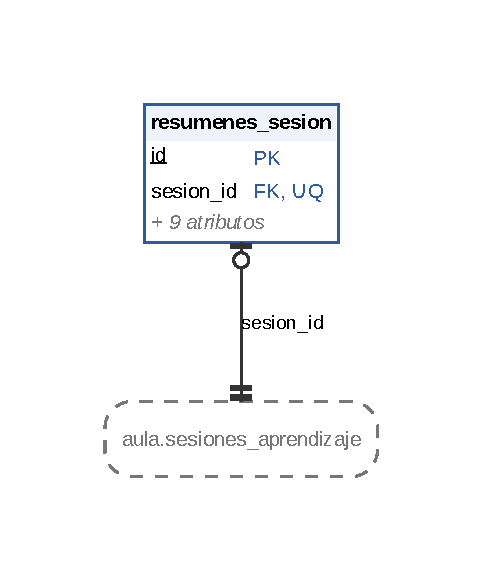
\includegraphics[scale=1.000]{figuras/der/resumen}
    \caption{Diagrama entidad-relación del esquema \texttt{resumen} (M6)}
    \label{fig:der-resumen}
\end{figure}

\subsubsection{\texorpdfstring{\texttt{resumen.resumenes\_\allowbreak{}sesion}}{resumen.resumenes\_sesion}}\label{dd:resumen.resumenes_sesion}

Resumen automático de una sesión (uno por sesión, no se regenera). Solo existe para sesiones de al menos 10 minutos efectivos con el adicional contratado. \emph{Migraciones:} V15.

{\small
\begin{xltabular}{\textwidth}{@{}>{\raggedright\arraybackslash}p{3.6cm} >{\raggedright\arraybackslash}p{2.3cm} >{\raggedright\arraybackslash}p{1cm} >{\centering\arraybackslash}p{0.85cm} L@{}}
    \toprule
    \tb{Atributo} & \tb{Tipo} & \tb{Clave} & \tb{Nulo} & \tb{Descripción} \\
    \midrule
    \endfirsthead
    \toprule
    \tb{Atributo} & \tb{Tipo} & \tb{Clave} & \tb{Nulo} & \tb{Descripción} \\
    \midrule
    \endhead
    \bottomrule
    \endfoot
    \texttt{id} & \texttt{uuid} & PK & no & Identificador (UUID generado por la base) \\
    \texttt{sesion\_\allowbreak{}id} & \texttt{uuid} & FK, UQ & no & Sesión resumida \\
    \texttt{estado} & \texttt{varchar(\allowbreak{}30)} &  & no & Estado del resumen. Por defecto: \texttt{\textquotesingle{}pendiente\textquotesingle{}} \\
    \texttt{prompt\_\allowbreak{}anonimizado} & \texttt{text} &  & sí & Prompt enviado al modelo, ya anonimizado \\
    \texttt{transcript\_\allowbreak{}anonimizado} & \texttt{text} &  & sí & Transcripción anonimizada; se guarda aunque no haya proveedor configurado \\
    \texttt{resumen\_\allowbreak{}final} & \texttt{text} &  & sí & Resumen generado; nulo hasta generarlo \\
    \texttt{intentos} & \texttt{integer} &  & no & Intentos de generación. Por defecto: \texttt{0} \\
    \texttt{proximo\_\allowbreak{}reintento\_\allowbreak{}at} & \texttt{timestamptz} &  & sí & Momento del próximo reintento (espera de 5, 15 y 60 minutos) \\
    \texttt{recordatorio\_\allowbreak{}pendiente} & \texttt{boolean} &  & no & Falta enviar el recordatorio único de 24 horas. Por defecto: \texttt{false} \\
    \texttt{suspendido\_\allowbreak{}seguridad} & \texttt{boolean} &  & no & Hay una denuncia o alerta activa sobre la sesión. Por defecto: \texttt{false} \\
    \texttt{created\_\allowbreak{}at} & \texttt{timestamptz} &  & no & Fecha y hora de creación de la fila. Por defecto: \texttt{now(\allowbreak{})} \\
\end{xltabular}
}

{\small
\begin{xltabular}{\textwidth}{@{}>{\raggedright\arraybackslash}p{1.7cm} >{\raggedright\arraybackslash}p{4.6cm} L@{}}
    \toprule
    \tb{Tipo} & \tb{Nombre} & \tb{Definición} \\
    \midrule
    \endfirsthead
    \toprule
    \tb{Tipo} & \tb{Nombre} & \tb{Definición} \\
    \midrule
    \endhead
    \bottomrule
    \endfoot
    CHECK & \texttt{resumenes\_\allowbreak{}sesion\_\allowbreak{}estado\_\allowbreak{}check} & \texttt{estado IN (\allowbreak{}\textquotesingle{}pendiente\textquotesingle{},\allowbreak{} \textquotesingle{}generado\textquotesingle{},\allowbreak{} \textquotesingle{}suspendido\_\allowbreak{}seguridad\textquotesingle{},\allowbreak{} \textquotesingle{}reintento\_\allowbreak{}agotado\textquotesingle{},\allowbreak{} \textquotesingle{}fallido\textquotesingle{})} \\
    CHECK & \texttt{resumenes\_\allowbreak{}sesion\_\allowbreak{}intentos\_\allowbreak{}check} & \texttt{intentos \textgreater{}= 0} \\
    FK & \texttt{resumenes\_\allowbreak{}sesion\_\allowbreak{}sesion\_\allowbreak{}id\_\allowbreak{}fkey} & \texttt{(\allowbreak{}sesion\_\allowbreak{}id) $\rightarrow$ aula.sesiones\_\allowbreak{}aprendizaje(\allowbreak{}id)} \\
    PK & \texttt{resumenes\_\allowbreak{}sesion\_\allowbreak{}pkey} & \texttt{(\allowbreak{}id)} \\
    UNIQUE & \texttt{resumenes\_\allowbreak{}sesion\_\allowbreak{}sesion\_\allowbreak{}id\_\allowbreak{}key} & \texttt{(\allowbreak{}sesion\_\allowbreak{}id)} \\
    Índice & \texttt{idx\_\allowbreak{}resumenes\_\allowbreak{}sesion\_\allowbreak{}estado} & \texttt{(\allowbreak{}estado)} \\
\end{xltabular}
}

\subsection{Esquema \texttt{reputacion} (M7)}\label{dd:reputacion}

Calificaciones bidireccionales y señales implícitas de comportamiento del tutor. Tablas: 2. Su diagrama entidad-relación es la figura~\ref{fig:der-reputacion}.

\begin{figure}[htbp]
    \centering
    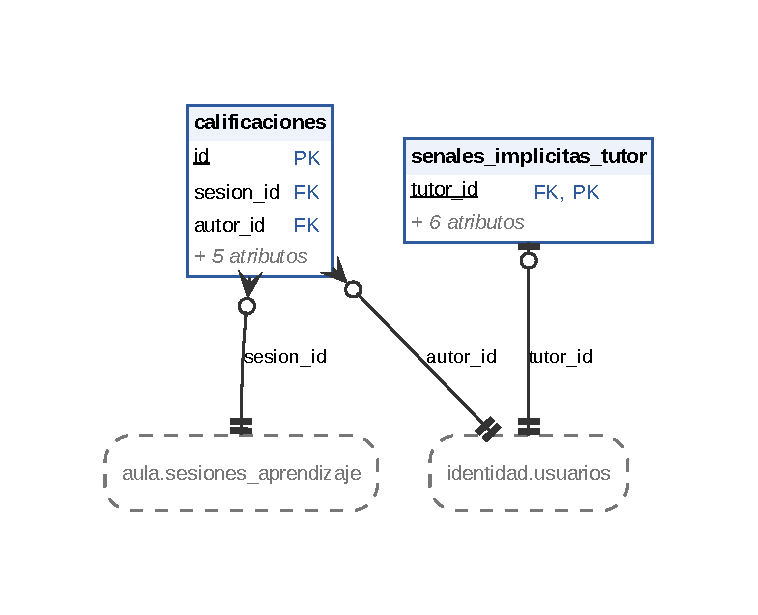
\includegraphics[scale=1.000]{figuras/der/reputacion}
    \caption{Diagrama entidad-relación del esquema \texttt{reputacion} (M7)}
    \label{fig:der-reputacion}
\end{figure}

\subsubsection{\texorpdfstring{\texttt{reputacion.calificaciones}}{reputacion.calificaciones}}\label{dd:reputacion.calificaciones}

Calificación de una sesión. Es bidireccional: el estudiante califica al tutor y el tutor al estudiante; la dirección se deriva del rol del autor. \emph{Migraciones:} V14.

{\small
\begin{xltabular}{\textwidth}{@{}>{\raggedright\arraybackslash}p{3.6cm} >{\raggedright\arraybackslash}p{2.3cm} >{\raggedright\arraybackslash}p{1cm} >{\centering\arraybackslash}p{0.85cm} L@{}}
    \toprule
    \tb{Atributo} & \tb{Tipo} & \tb{Clave} & \tb{Nulo} & \tb{Descripción} \\
    \midrule
    \endfirsthead
    \toprule
    \tb{Atributo} & \tb{Tipo} & \tb{Clave} & \tb{Nulo} & \tb{Descripción} \\
    \midrule
    \endhead
    \bottomrule
    \endfoot
    \texttt{id} & \texttt{uuid} & PK & no & Identificador (UUID generado por la base) \\
    \texttt{sesion\_\allowbreak{}id} & \texttt{uuid} & FK & no & Sesión calificada \\
    \texttt{autor\_\allowbreak{}id} & \texttt{uuid} & FK & no & Usuario que califica \\
    \texttt{direccion} & \texttt{varchar(\allowbreak{}30)} &  & no & estudiante\_a\_tutor o tutor\_a\_estudiante \\
    \texttt{estrellas} & \texttt{smallint} &  & no & Puntaje de 1 a 5 \\
    \texttt{comentario} & \texttt{varchar(\allowbreak{}1000)} &  & sí & Comentario; solo en la dirección estudiante\_a\_tutor \\
    \texttt{editable\_\allowbreak{}hasta} & \texttt{timestamptz} &  & no & Fin del plazo de edición: 48 horas desde la creación \\
    \texttt{created\_\allowbreak{}at} & \texttt{timestamptz} &  & no & Fecha y hora de creación de la fila. Por defecto: \texttt{now(\allowbreak{})} \\
\end{xltabular}
}

{\small
\begin{xltabular}{\textwidth}{@{}>{\raggedright\arraybackslash}p{1.7cm} >{\raggedright\arraybackslash}p{4.6cm} L@{}}
    \toprule
    \tb{Tipo} & \tb{Nombre} & \tb{Definición} \\
    \midrule
    \endfirsthead
    \toprule
    \tb{Tipo} & \tb{Nombre} & \tb{Definición} \\
    \midrule
    \endhead
    \bottomrule
    \endfoot
    CHECK & \texttt{calificaciones\_\allowbreak{}direccion\_\allowbreak{}check} & \texttt{direccion IN (\allowbreak{}\textquotesingle{}estudiante\_\allowbreak{}a\_\allowbreak{}tutor\textquotesingle{},\allowbreak{} \textquotesingle{}tutor\_\allowbreak{}a\_\allowbreak{}estudiante\textquotesingle{})} \\
    CHECK & \texttt{calificaciones\_\allowbreak{}estrellas\_\allowbreak{}check} & \texttt{(\allowbreak{}estrellas \textgreater{}= 1) AND (\allowbreak{}estrellas \textless{}= 5)} \\
    FK & \texttt{calificaciones\_\allowbreak{}autor\_\allowbreak{}id\_\allowbreak{}fkey} & \texttt{(\allowbreak{}autor\_\allowbreak{}id) $\rightarrow$ identidad.usuarios(\allowbreak{}id)} \\
    FK & \texttt{calificaciones\_\allowbreak{}sesion\_\allowbreak{}id\_\allowbreak{}fkey} & \texttt{(\allowbreak{}sesion\_\allowbreak{}id) $\rightarrow$ aula.sesiones\_\allowbreak{}aprendizaje(\allowbreak{}id)} \\
    PK & \texttt{calificaciones\_\allowbreak{}pkey} & \texttt{(\allowbreak{}id)} \\
    UNIQUE & \texttt{uq\_\allowbreak{}calificacion\_\allowbreak{}por\_\allowbreak{}sesion\_\allowbreak{}autor\_\allowbreak{}direccion} & \texttt{(\allowbreak{}sesion\_\allowbreak{}id,\allowbreak{} autor\_\allowbreak{}id,\allowbreak{} direccion)} \\
    Índice & \texttt{idx\_\allowbreak{}calificaciones\_\allowbreak{}sesion} & \texttt{(\allowbreak{}sesion\_\allowbreak{}id)} \\
    Índice & \texttt{idx\_\allowbreak{}calificaciones\_\allowbreak{}tutor\_\allowbreak{}direccion} & \texttt{(\allowbreak{}direccion)} \\
\end{xltabular}
}

\subsubsection{\texorpdfstring{\texttt{reputacion.senales\_\allowbreak{}implicitas\_\allowbreak{}tutor}}{reputacion.senales\_implicitas\_tutor}}\label{dd:reputacion.senales_implicitas_tutor}

Señales de comportamiento del tutor, agregadas y recalculadas de forma incremental (ADR-M7-01). No es un registro de eventos. \emph{Migraciones:} V14.

{\small
\begin{xltabular}{\textwidth}{@{}>{\raggedright\arraybackslash}p{3.6cm} >{\raggedright\arraybackslash}p{2.3cm} >{\raggedright\arraybackslash}p{1cm} >{\centering\arraybackslash}p{0.85cm} L@{}}
    \toprule
    \tb{Atributo} & \tb{Tipo} & \tb{Clave} & \tb{Nulo} & \tb{Descripción} \\
    \midrule
    \endfirsthead
    \toprule
    \tb{Atributo} & \tb{Tipo} & \tb{Clave} & \tb{Nulo} & \tb{Descripción} \\
    \midrule
    \endhead
    \bottomrule
    \endfoot
    \texttt{tutor\_\allowbreak{}id} & \texttt{uuid} & FK, PK & no & Tutor al que corresponden las señales \\
    \texttt{puntualidad\_\allowbreak{}promedio} & \texttt{numeric(\allowbreak{}5,\allowbreak{}4)} &  & no & Puntualidad promedio (0 a 1). Por defecto: \texttt{1.0} \\
    \texttt{tasa\_\allowbreak{}recontratacion} & \texttt{numeric(\allowbreak{}5,\allowbreak{}4)} &  & no & Proporción de alumnos que vuelven a reservar. Por defecto: \texttt{0.0} \\
    \texttt{tasa\_\allowbreak{}cancelacion\_\allowbreak{}noshow} & \texttt{numeric(\allowbreak{}5,\allowbreak{}4)} &  & no & Proporción de clases canceladas o con ausencia del tutor. Por defecto: \texttt{0.0} \\
    \texttt{tiempo\_\allowbreak{}respuesta\_\allowbreak{}promedio\_\allowbreak{}min} & \texttt{integer} &  & no & Tiempo promedio de respuesta, en minutos. Por defecto: \texttt{0} \\
    \texttt{sesiones\_\allowbreak{}dictadas\_\allowbreak{}total} & \texttt{integer} &  & no & Cantidad de sesiones dictadas. Por defecto: \texttt{0} \\
    \texttt{updated\_\allowbreak{}at} & \texttt{timestamptz} &  & no & Fecha y hora del último recálculo. Por defecto: \texttt{now(\allowbreak{})} \\
\end{xltabular}
}

{\small
\begin{xltabular}{\textwidth}{@{}>{\raggedright\arraybackslash}p{1.7cm} >{\raggedright\arraybackslash}p{4.6cm} L@{}}
    \toprule
    \tb{Tipo} & \tb{Nombre} & \tb{Definición} \\
    \midrule
    \endfirsthead
    \toprule
    \tb{Tipo} & \tb{Nombre} & \tb{Definición} \\
    \midrule
    \endhead
    \bottomrule
    \endfoot
    FK & \texttt{senales\_\allowbreak{}implicitas\_\allowbreak{}tutor\_\allowbreak{}tutor\_\allowbreak{}id\_\allowbreak{}fkey} & \texttt{(\allowbreak{}tutor\_\allowbreak{}id) $\rightarrow$ identidad.usuarios(\allowbreak{}id)} \\
    PK & \texttt{senales\_\allowbreak{}implicitas\_\allowbreak{}tutor\_\allowbreak{}pkey} & \texttt{(\allowbreak{}tutor\_\allowbreak{}id)} \\
\end{xltabular}
}

\subsection{Esquema \texttt{admin} (M8)}\label{dd:admin}

Panel de administración: administradores, auditoría, tickets de soporte, notificaciones y respuestas \gls{nps}. Tablas: 6. Su diagrama entidad-relación es la figura~\ref{fig:der-admin}.

\begin{figure}[htbp]
    \centering
    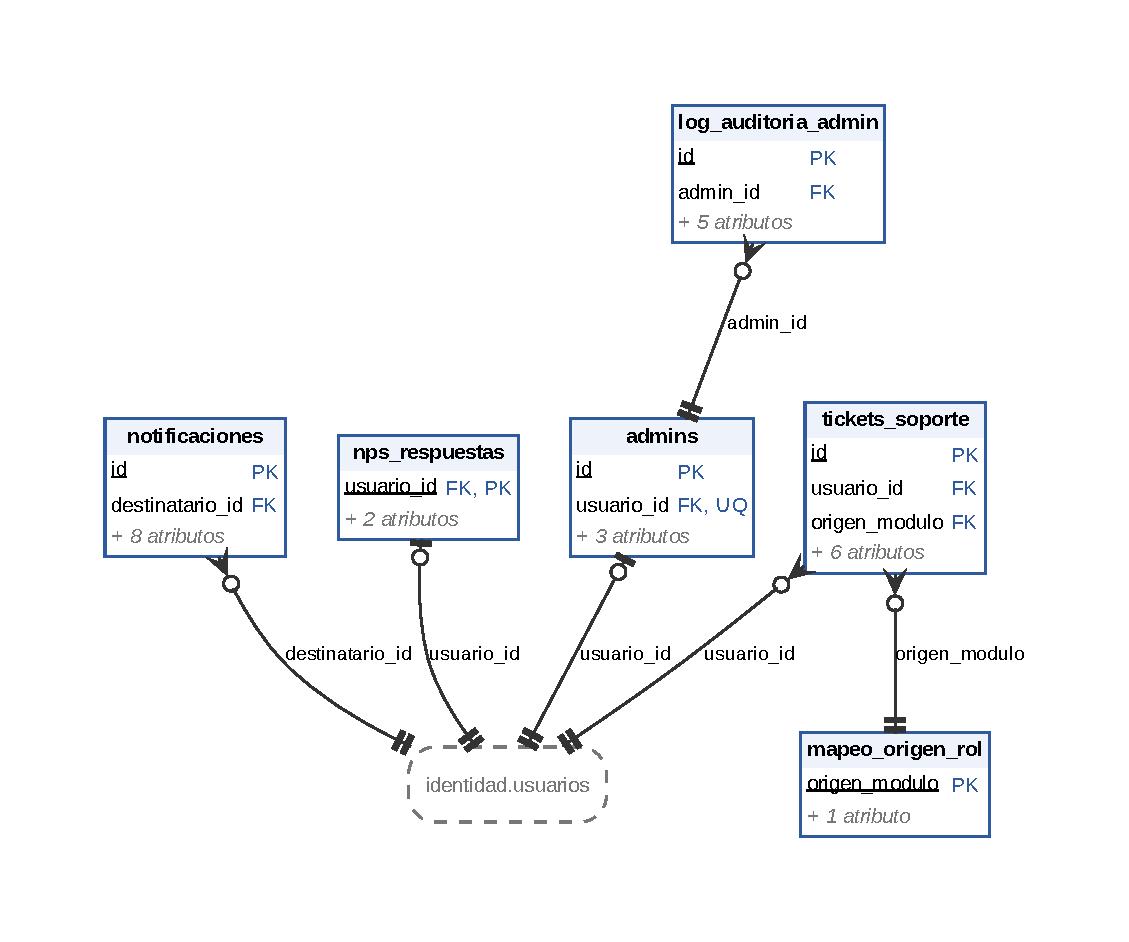
\includegraphics[scale=0.784]{figuras/der/admin}
    \caption{Diagrama entidad-relación del esquema \texttt{admin} (M8)}
    \label{fig:der-admin}
\end{figure}

\subsubsection{\texorpdfstring{\texttt{admin.admins}}{admin.admins}}\label{dd:admin.admins}

Personal interno con acceso al panel. Cada administrador está vinculado a un usuario y tiene exactamente uno de dos roles. \emph{Migraciones:} V16.

{\small
\begin{xltabular}{\textwidth}{@{}>{\raggedright\arraybackslash}p{3.6cm} >{\raggedright\arraybackslash}p{2.3cm} >{\raggedright\arraybackslash}p{1cm} >{\centering\arraybackslash}p{0.85cm} L@{}}
    \toprule
    \tb{Atributo} & \tb{Tipo} & \tb{Clave} & \tb{Nulo} & \tb{Descripción} \\
    \midrule
    \endfirsthead
    \toprule
    \tb{Atributo} & \tb{Tipo} & \tb{Clave} & \tb{Nulo} & \tb{Descripción} \\
    \midrule
    \endhead
    \bottomrule
    \endfoot
    \texttt{id} & \texttt{uuid} & PK & no & Identificador (UUID generado por la base) \\
    \texttt{usuario\_\allowbreak{}id} & \texttt{uuid} & FK, UQ & no & Usuario vinculado (uno por administrador) \\
    \texttt{rol} & \texttt{varchar(\allowbreak{}30)} &  & no & MODERACION\_SEGURIDAD o SOPORTE\_FINANCIERO \\
    \texttt{activo} & \texttt{boolean} &  & no & El administrador puede operar. Por defecto: \texttt{true} \\
    \texttt{created\_\allowbreak{}at} & \texttt{timestamptz} &  & no & Fecha y hora de creación de la fila. Por defecto: \texttt{now(\allowbreak{})} \\
\end{xltabular}
}

{\small
\begin{xltabular}{\textwidth}{@{}>{\raggedright\arraybackslash}p{1.7cm} >{\raggedright\arraybackslash}p{4.6cm} L@{}}
    \toprule
    \tb{Tipo} & \tb{Nombre} & \tb{Definición} \\
    \midrule
    \endfirsthead
    \toprule
    \tb{Tipo} & \tb{Nombre} & \tb{Definición} \\
    \midrule
    \endhead
    \bottomrule
    \endfoot
    CHECK & \texttt{admins\_\allowbreak{}rol\_\allowbreak{}check} & \texttt{rol IN (\allowbreak{}\textquotesingle{}MODERACION\_\allowbreak{}SEGURIDAD\textquotesingle{},\allowbreak{} \textquotesingle{}SOPORTE\_\allowbreak{}FINANCIERO\textquotesingle{})} \\
    FK & \texttt{admins\_\allowbreak{}usuario\_\allowbreak{}id\_\allowbreak{}fkey} & \texttt{(\allowbreak{}usuario\_\allowbreak{}id) $\rightarrow$ identidad.usuarios(\allowbreak{}id)} \\
    PK & \texttt{admins\_\allowbreak{}pkey} & \texttt{(\allowbreak{}id)} \\
    UNIQUE & \texttt{admins\_\allowbreak{}usuario\_\allowbreak{}id\_\allowbreak{}key} & \texttt{(\allowbreak{}usuario\_\allowbreak{}id)} \\
    Índice & \texttt{idx\_\allowbreak{}admins\_\allowbreak{}rol} & \texttt{(\allowbreak{}rol)} \\
\end{xltabular}
}

\subsubsection{\texorpdfstring{\texttt{admin.log\_\allowbreak{}auditoria\_\allowbreak{}admin}}{admin.log\_auditoria\_admin}}\label{dd:admin.log_auditoria_admin}

Auditoría de cada acción de un administrador. Es de solo agregado a nivel del motor: la tabla pertenece a un rol sin inicio de sesión y la aplicación solo tiene permisos de SELECT e INSERT. \emph{Migraciones:} V16.

{\small
\begin{xltabular}{\textwidth}{@{}>{\raggedright\arraybackslash}p{3.6cm} >{\raggedright\arraybackslash}p{2.3cm} >{\raggedright\arraybackslash}p{1cm} >{\centering\arraybackslash}p{0.85cm} L@{}}
    \toprule
    \tb{Atributo} & \tb{Tipo} & \tb{Clave} & \tb{Nulo} & \tb{Descripción} \\
    \midrule
    \endfirsthead
    \toprule
    \tb{Atributo} & \tb{Tipo} & \tb{Clave} & \tb{Nulo} & \tb{Descripción} \\
    \midrule
    \endhead
    \bottomrule
    \endfoot
    \texttt{id} & \texttt{uuid} & PK & no & Identificador (UUID generado por la base) \\
    \texttt{admin\_\allowbreak{}id} & \texttt{uuid} & FK & no & Administrador que actuó \\
    \texttt{accion} & \texttt{varchar(\allowbreak{}100)} &  & no & Acción realizada \\
    \texttt{entidad\_\allowbreak{}tipo} & \texttt{varchar(\allowbreak{}60)} &  & no & Tipo de la entidad afectada \\
    \texttt{entidad\_\allowbreak{}id} & \texttt{varchar(\allowbreak{}64)} &  & sí & Identificador de la entidad afectada \\
    \texttt{detalle} & \texttt{jsonb} &  & sí & Datos adicionales de la acción, en JSON \\
    \texttt{created\_\allowbreak{}at} & \texttt{timestamptz} &  & no & Fecha y hora de la acción. Por defecto: \texttt{now(\allowbreak{})} \\
\end{xltabular}
}

{\small
\begin{xltabular}{\textwidth}{@{}>{\raggedright\arraybackslash}p{1.7cm} >{\raggedright\arraybackslash}p{4.6cm} L@{}}
    \toprule
    \tb{Tipo} & \tb{Nombre} & \tb{Definición} \\
    \midrule
    \endfirsthead
    \toprule
    \tb{Tipo} & \tb{Nombre} & \tb{Definición} \\
    \midrule
    \endhead
    \bottomrule
    \endfoot
    FK & \texttt{log\_\allowbreak{}auditoria\_\allowbreak{}admin\_\allowbreak{}admin\_\allowbreak{}id\_\allowbreak{}fkey} & \texttt{(\allowbreak{}admin\_\allowbreak{}id) $\rightarrow$ admin.admins(\allowbreak{}id)} \\
    PK & \texttt{log\_\allowbreak{}auditoria\_\allowbreak{}admin\_\allowbreak{}pkey} & \texttt{(\allowbreak{}id)} \\
\end{xltabular}
}

\subsubsection{\texorpdfstring{\texttt{admin.mapeo\_\allowbreak{}origen\_\allowbreak{}rol}}{admin.mapeo\_origen\_rol}}\label{dd:admin.mapeo_origen_rol}

Configuración del enrutamiento de tickets: qué rol atiende cada origen. Se edita sin desplegar código. \emph{Migraciones:} V16.

{\small
\begin{xltabular}{\textwidth}{@{}>{\raggedright\arraybackslash}p{3.6cm} >{\raggedright\arraybackslash}p{2.3cm} >{\raggedright\arraybackslash}p{1cm} >{\centering\arraybackslash}p{0.85cm} L@{}}
    \toprule
    \tb{Atributo} & \tb{Tipo} & \tb{Clave} & \tb{Nulo} & \tb{Descripción} \\
    \midrule
    \endfirsthead
    \toprule
    \tb{Atributo} & \tb{Tipo} & \tb{Clave} & \tb{Nulo} & \tb{Descripción} \\
    \midrule
    \endhead
    \bottomrule
    \endfoot
    \texttt{origen\_\allowbreak{}modulo} & \texttt{varchar(\allowbreak{}60)} & PK & no & Origen del ticket (por ejemplo, \path{M5.pago_fallido}) \\
    \texttt{rol\_\allowbreak{}asignado} & \texttt{varchar(\allowbreak{}30)} &  & no & Rol que atiende los tickets de ese origen \\
\end{xltabular}
}

{\small
\begin{xltabular}{\textwidth}{@{}>{\raggedright\arraybackslash}p{1.7cm} >{\raggedright\arraybackslash}p{4.6cm} L@{}}
    \toprule
    \tb{Tipo} & \tb{Nombre} & \tb{Definición} \\
    \midrule
    \endfirsthead
    \toprule
    \tb{Tipo} & \tb{Nombre} & \tb{Definición} \\
    \midrule
    \endhead
    \bottomrule
    \endfoot
    CHECK & \texttt{mapeo\_\allowbreak{}origen\_\allowbreak{}rol\_\allowbreak{}rol\_\allowbreak{}asignado\_\allowbreak{}check} & \texttt{rol\_\allowbreak{}asignado IN (\allowbreak{}\textquotesingle{}MODERACION\_\allowbreak{}SEGURIDAD\textquotesingle{},\allowbreak{} \textquotesingle{}SOPORTE\_\allowbreak{}FINANCIERO\textquotesingle{})} \\
    PK & \texttt{mapeo\_\allowbreak{}origen\_\allowbreak{}rol\_\allowbreak{}pkey} & \texttt{(\allowbreak{}origen\_\allowbreak{}modulo)} \\
\end{xltabular}
}

\subsubsection{\texorpdfstring{\texttt{admin.notificaciones}}{admin.notificaciones}}\label{dd:admin.notificaciones}

Avisos a los usuarios: es a la vez la bandeja dentro de la aplicación y la cola de salida del correo (ADR-000-06). Se escribe en la misma transacción que el hecho que la origina. \emph{Migraciones:} V32.

{\small
\begin{xltabular}{\textwidth}{@{}>{\raggedright\arraybackslash}p{3.6cm} >{\raggedright\arraybackslash}p{2.3cm} >{\raggedright\arraybackslash}p{1cm} >{\centering\arraybackslash}p{0.85cm} L@{}}
    \toprule
    \tb{Atributo} & \tb{Tipo} & \tb{Clave} & \tb{Nulo} & \tb{Descripción} \\
    \midrule
    \endfirsthead
    \toprule
    \tb{Atributo} & \tb{Tipo} & \tb{Clave} & \tb{Nulo} & \tb{Descripción} \\
    \midrule
    \endhead
    \bottomrule
    \endfoot
    \texttt{id} & \texttt{uuid} & PK & no & Identificador (UUID generado por la aplicación) \\
    \texttt{destinatario\_\allowbreak{}id} & \texttt{uuid} & FK & no & Usuario destinatario \\
    \texttt{tipo} & \texttt{varchar(\allowbreak{}40)} &  & no & Tipo de aviso \\
    \texttt{datos} & \texttt{jsonb} &  & no & Datos del aviso, en JSON. Por defecto: \texttt{\textquotesingle{}\{\}\textquotesingle{}} \\
    \texttt{creada\_\allowbreak{}at} & \texttt{timestamptz} &  & no & Fecha y hora de creación de la fila. Por defecto: \texttt{now(\allowbreak{})} \\
    \texttt{leida\_\allowbreak{}at} & \texttt{timestamptz} &  & sí & Fecha y hora en que el usuario la leyó \\
    \texttt{enviada\_\allowbreak{}email\_\allowbreak{}at} & \texttt{timestamptz} &  & sí & Fecha y hora del envío por correo \\
    \texttt{intentos\_\allowbreak{}email} & \texttt{integer} &  & no & Intentos de envío por correo. Por defecto: \texttt{0} \\
    \texttt{proximo\_\allowbreak{}intento\_\allowbreak{}email\_\allowbreak{}at} & \texttt{timestamptz} &  & sí & Momento del próximo intento (espera de 5, 15 y 60 minutos) \\
    \texttt{email\_\allowbreak{}descartado\_\allowbreak{}at} & \texttt{timestamptz} &  & sí & Se descartó el correo: intentos agotados o destinatario sin correo \\
\end{xltabular}
}

{\small
\begin{xltabular}{\textwidth}{@{}>{\raggedright\arraybackslash}p{1.7cm} >{\raggedright\arraybackslash}p{4.6cm} L@{}}
    \toprule
    \tb{Tipo} & \tb{Nombre} & \tb{Definición} \\
    \midrule
    \endfirsthead
    \toprule
    \tb{Tipo} & \tb{Nombre} & \tb{Definición} \\
    \midrule
    \endhead
    \bottomrule
    \endfoot
    FK & \texttt{notificaciones\_\allowbreak{}destinatario\_\allowbreak{}id\_\allowbreak{}fkey} & \texttt{(\allowbreak{}destinatario\_\allowbreak{}id) $\rightarrow$ identidad.usuarios(\allowbreak{}id)} \\
    PK & \texttt{notificaciones\_\allowbreak{}pkey} & \texttt{(\allowbreak{}id)} \\
    Índice & \texttt{ix\_\allowbreak{}notificaciones\_\allowbreak{}destinatario} & \texttt{(\allowbreak{}destinatario\_\allowbreak{}id,\allowbreak{} creada\_\allowbreak{}at DESC)} \\
    Índice & \texttt{ix\_\allowbreak{}notificaciones\_\allowbreak{}email\_\allowbreak{}pendiente} & \texttt{(\allowbreak{}proximo\_\allowbreak{}intento\_\allowbreak{}email\_\allowbreak{}at) WHERE (\allowbreak{}enviada\_\allowbreak{}email\_\allowbreak{}at IS NULL) AND (\allowbreak{}email\_\allowbreak{}descartado\_\allowbreak{}at IS NULL)} \\
\end{xltabular}
}

\subsubsection{\texorpdfstring{\texttt{admin.nps\_\allowbreak{}respuestas}}{admin.nps\_respuestas}}\label{dd:admin.nps_respuestas}

Respuesta a la pregunta \gls{nps} de intención (indicador I-04), una por usuario. \emph{Migraciones:} V58.

{\small
\begin{xltabular}{\textwidth}{@{}>{\raggedright\arraybackslash}p{3.6cm} >{\raggedright\arraybackslash}p{2.3cm} >{\raggedright\arraybackslash}p{1cm} >{\centering\arraybackslash}p{0.85cm} L@{}}
    \toprule
    \tb{Atributo} & \tb{Tipo} & \tb{Clave} & \tb{Nulo} & \tb{Descripción} \\
    \midrule
    \endfirsthead
    \toprule
    \tb{Atributo} & \tb{Tipo} & \tb{Clave} & \tb{Nulo} & \tb{Descripción} \\
    \midrule
    \endhead
    \bottomrule
    \endfoot
    \texttt{usuario\_\allowbreak{}id} & \texttt{uuid} & FK, PK & no & Usuario que respondió \\
    \texttt{puntaje} & \texttt{smallint} &  & no & Puntaje de 0 a 10 \\
    \texttt{created\_\allowbreak{}at} & \texttt{timestamptz} &  & no & Fecha y hora de la respuesta. Por defecto: \texttt{now(\allowbreak{})} \\
\end{xltabular}
}

{\small
\begin{xltabular}{\textwidth}{@{}>{\raggedright\arraybackslash}p{1.7cm} >{\raggedright\arraybackslash}p{4.6cm} L@{}}
    \toprule
    \tb{Tipo} & \tb{Nombre} & \tb{Definición} \\
    \midrule
    \endfirsthead
    \toprule
    \tb{Tipo} & \tb{Nombre} & \tb{Definición} \\
    \midrule
    \endhead
    \bottomrule
    \endfoot
    CHECK & \texttt{nps\_\allowbreak{}respuestas\_\allowbreak{}puntaje\_\allowbreak{}check} & \texttt{(\allowbreak{}puntaje \textgreater{}= 0) AND (\allowbreak{}puntaje \textless{}= 10)} \\
    FK & \texttt{nps\_\allowbreak{}respuestas\_\allowbreak{}usuario\_\allowbreak{}id\_\allowbreak{}fkey} & \texttt{(\allowbreak{}usuario\_\allowbreak{}id) $\rightarrow$ identidad.usuarios(\allowbreak{}id)} \\
    PK & \texttt{nps\_\allowbreak{}respuestas\_\allowbreak{}pkey} & \texttt{(\allowbreak{}usuario\_\allowbreak{}id)} \\
    Índice & \texttt{idx\_\allowbreak{}nps\_\allowbreak{}respuestas\_\allowbreak{}created} & \texttt{(\allowbreak{}created\_\allowbreak{}at)} \\
\end{xltabular}
}

\subsubsection{\texorpdfstring{\texttt{admin.tickets\_\allowbreak{}soporte}}{admin.tickets\_soporte}}\label{dd:admin.tickets_soporte}

Pedidos del canal ``contactar a soporte''. El origen debe existir en el mapeo, de modo que siempre se puede derivar el rol. \emph{Migraciones:} V16.

{\small
\begin{xltabular}{\textwidth}{@{}>{\raggedright\arraybackslash}p{3.6cm} >{\raggedright\arraybackslash}p{2.3cm} >{\raggedright\arraybackslash}p{1cm} >{\centering\arraybackslash}p{0.85cm} L@{}}
    \toprule
    \tb{Atributo} & \tb{Tipo} & \tb{Clave} & \tb{Nulo} & \tb{Descripción} \\
    \midrule
    \endfirsthead
    \toprule
    \tb{Atributo} & \tb{Tipo} & \tb{Clave} & \tb{Nulo} & \tb{Descripción} \\
    \midrule
    \endhead
    \bottomrule
    \endfoot
    \texttt{id} & \texttt{uuid} & PK & no & Identificador (UUID generado por la base) \\
    \texttt{usuario\_\allowbreak{}id} & \texttt{uuid} & FK & no & Usuario que abre el ticket \\
    \texttt{origen\_\allowbreak{}modulo} & \texttt{varchar(\allowbreak{}60)} & FK & no & Origen del ticket \\
    \texttt{asunto} & \texttt{varchar(\allowbreak{}200)} &  & no & Asunto \\
    \texttt{detalle} & \texttt{varchar(\allowbreak{}1000)} &  & no & Descripción del problema \\
    \texttt{estado} & \texttt{varchar(\allowbreak{}20)} &  & no & ABIERTO, EN\_PROCESO, RESUELTO o CERRADO. Por defecto: \texttt{\textquotesingle{}ABIERTO\textquotesingle{}} \\
    \texttt{rol\_\allowbreak{}asignado} & \texttt{varchar(\allowbreak{}30)} &  & no & Rol que lo atiende, derivado del origen \\
    \texttt{creado\_\allowbreak{}en} & \texttt{timestamptz} &  & no & Fecha y hora de creación de la fila. Por defecto: \texttt{now(\allowbreak{})} \\
    \texttt{resuelto\_\allowbreak{}en} & \texttt{timestamptz} &  & sí & Fecha y hora de la resolución \\
\end{xltabular}
}

{\small
\begin{xltabular}{\textwidth}{@{}>{\raggedright\arraybackslash}p{1.7cm} >{\raggedright\arraybackslash}p{4.6cm} L@{}}
    \toprule
    \tb{Tipo} & \tb{Nombre} & \tb{Definición} \\
    \midrule
    \endfirsthead
    \toprule
    \tb{Tipo} & \tb{Nombre} & \tb{Definición} \\
    \midrule
    \endhead
    \bottomrule
    \endfoot
    CHECK & \texttt{tickets\_\allowbreak{}soporte\_\allowbreak{}estado\_\allowbreak{}check} & \texttt{estado IN (\allowbreak{}\textquotesingle{}ABIERTO\textquotesingle{},\allowbreak{} \textquotesingle{}EN\_\allowbreak{}PROCESO\textquotesingle{},\allowbreak{} \textquotesingle{}RESUELTO\textquotesingle{},\allowbreak{} \textquotesingle{}CERRADO\textquotesingle{})} \\
    CHECK & \texttt{tickets\_\allowbreak{}soporte\_\allowbreak{}rol\_\allowbreak{}asignado\_\allowbreak{}check} & \texttt{rol\_\allowbreak{}asignado IN (\allowbreak{}\textquotesingle{}MODERACION\_\allowbreak{}SEGURIDAD\textquotesingle{},\allowbreak{} \textquotesingle{}SOPORTE\_\allowbreak{}FINANCIERO\textquotesingle{})} \\
    FK & \texttt{tickets\_\allowbreak{}soporte\_\allowbreak{}origen\_\allowbreak{}modulo\_\allowbreak{}fkey} & \texttt{(\allowbreak{}origen\_\allowbreak{}modulo) $\rightarrow$ admin.mapeo\_\allowbreak{}origen\_\allowbreak{}rol(\allowbreak{}origen\_\allowbreak{}modulo)} \\
    FK & \texttt{tickets\_\allowbreak{}soporte\_\allowbreak{}usuario\_\allowbreak{}id\_\allowbreak{}fkey} & \texttt{(\allowbreak{}usuario\_\allowbreak{}id) $\rightarrow$ identidad.usuarios(\allowbreak{}id)} \\
    PK & \texttt{tickets\_\allowbreak{}soporte\_\allowbreak{}pkey} & \texttt{(\allowbreak{}id)} \\
    Índice & \texttt{idx\_\allowbreak{}tickets\_\allowbreak{}rol\_\allowbreak{}estado} & \texttt{(\allowbreak{}rol\_\allowbreak{}asignado,\allowbreak{} estado)} \\
\end{xltabular}
}

\subsection{Esquema \texttt{seguridad} (M9)}\label{dd:seguridad}

Denuncias y sanciones. Tablas: 2. Su diagrama entidad-relación es la figura~\ref{fig:der-seguridad}.

\begin{figure}[htbp]
    \centering
    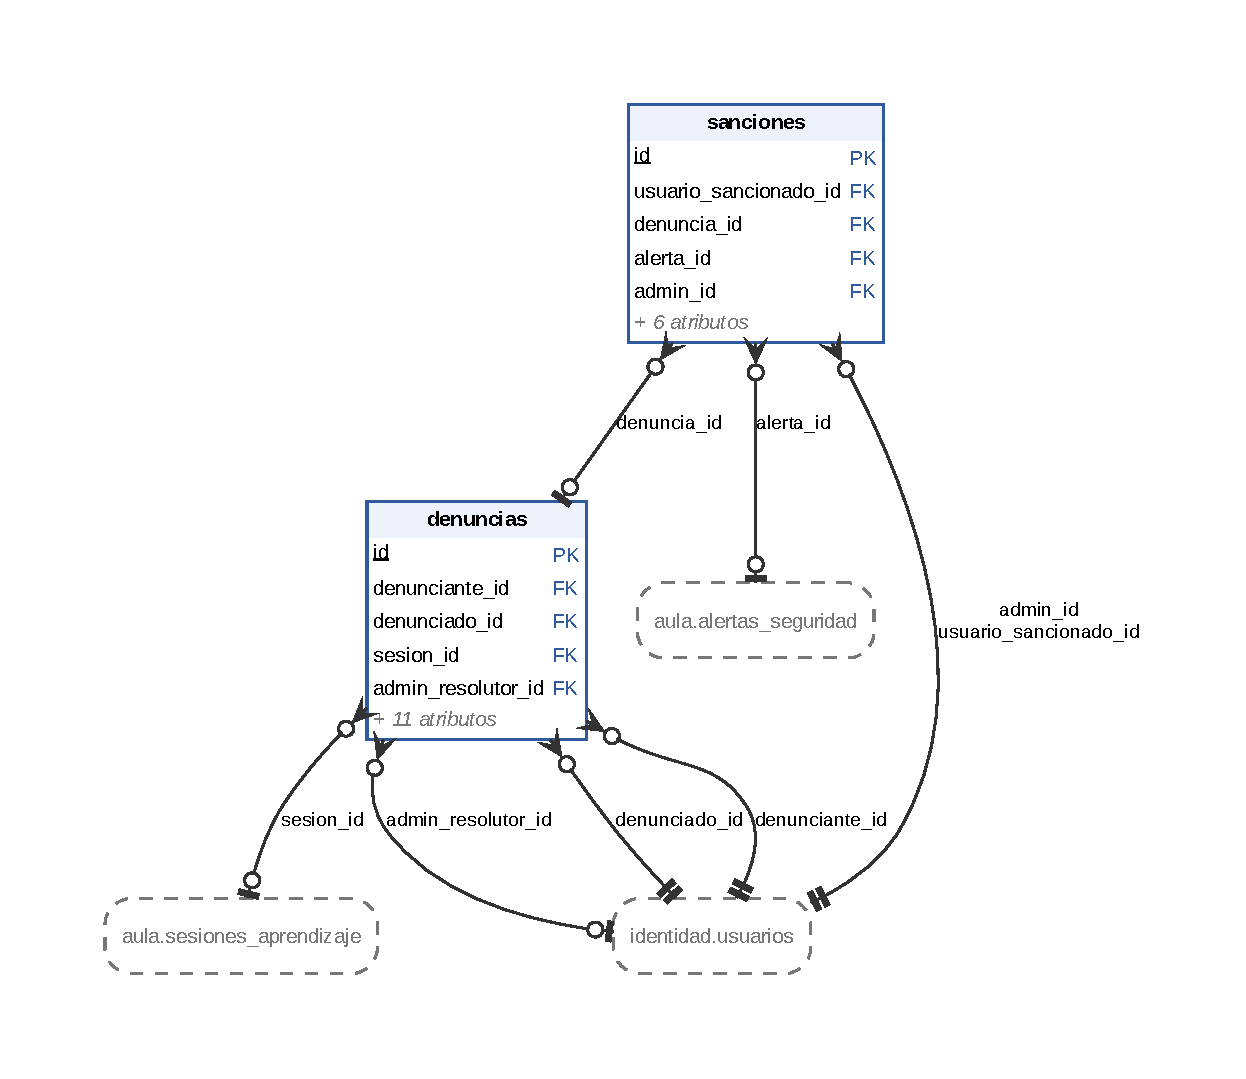
\includegraphics[scale=0.711]{figuras/der/seguridad}
    \caption{Diagrama entidad-relación del esquema \texttt{seguridad} (M9)}
    \label{fig:der-seguridad}
\end{figure}

\subsubsection{\texorpdfstring{\texttt{seguridad.denuncias}}{seguridad.denuncias}}\label{dd:seguridad.denuncias}

Denuncia de un usuario contra otro. El denunciado tiene 48 horas para el descargo y moderación tiene 5 días hábiles más para resolver. \emph{Migraciones:} V13, V48.

{\small
\begin{xltabular}{\textwidth}{@{}>{\raggedright\arraybackslash}p{3.6cm} >{\raggedright\arraybackslash}p{2.3cm} >{\raggedright\arraybackslash}p{1cm} >{\centering\arraybackslash}p{0.85cm} L@{}}
    \toprule
    \tb{Atributo} & \tb{Tipo} & \tb{Clave} & \tb{Nulo} & \tb{Descripción} \\
    \midrule
    \endfirsthead
    \toprule
    \tb{Atributo} & \tb{Tipo} & \tb{Clave} & \tb{Nulo} & \tb{Descripción} \\
    \midrule
    \endhead
    \bottomrule
    \endfoot
    \texttt{id} & \texttt{uuid} & PK & no & Identificador (UUID generado por la base) \\
    \texttt{denunciante\_\allowbreak{}id} & \texttt{uuid} & FK & no & Usuario que denuncia \\
    \texttt{denunciado\_\allowbreak{}id} & \texttt{uuid} & FK & no & Usuario denunciado \\
    \texttt{sesion\_\allowbreak{}id} & \texttt{uuid} & FK & sí & Sesión en la que ocurrió el hecho, si la hay \\
    \texttt{motivo} & \texttt{varchar(\allowbreak{}40)} &  & no & Motivo codificado de la denuncia \\
    \texttt{evidencia\_\allowbreak{}url} & \texttt{varchar(\allowbreak{}500)} &  & sí & Referencia a la evidencia adjunta, si la hay \\
    \texttt{estado} & \texttt{varchar(\allowbreak{}30)} &  & no & Estado de la denuncia. Por defecto: \texttt{\textquotesingle{}REGISTRADA\textquotesingle{}} \\
    \texttt{descargo\_\allowbreak{}texto} & \texttt{varchar(\allowbreak{}300)} &  & sí & Último descargo del denunciado (hasta 300 caracteres) \\
    \texttt{descargo\_\allowbreak{}recibido\_\allowbreak{}at} & \texttt{timestamptz} &  & sí & Fecha y hora del último descargo \\
    \texttt{descargo\_\allowbreak{}vence\_\allowbreak{}at} & \texttt{timestamptz} &  & sí & Fin del plazo de descargo: 48 horas desde que entra en revisión \\
    \texttt{sla\_\allowbreak{}resolucion\_\allowbreak{}vence\_\allowbreak{}at} & \texttt{timestamptz} &  & sí & Fin del plazo de resolución: 5 días hábiles desde el vencimiento del descargo \\
    \texttt{prioridad\_\allowbreak{}alta} & \texttt{boolean} &  & no & La marcó el trabajo de plazos por vencer; no se resuelve sola. Por defecto: \texttt{false} \\
    \texttt{admin\_\allowbreak{}resolutor\_\allowbreak{}id} & \texttt{uuid} & FK & sí & Usuario administrador que resolvió \\
    \texttt{resuelta\_\allowbreak{}at} & \texttt{timestamptz} &  & sí & Fecha y hora de la resolución \\
    \texttt{created\_\allowbreak{}at} & \texttt{timestamptz} &  & no & Fecha y hora de creación de la fila. Por defecto: \texttt{now(\allowbreak{})} \\
    \texttt{descargo\_\allowbreak{}historial} & \texttt{text} &  & sí & Todos los descargos con su fecha, para el administrador \\
\end{xltabular}
}

{\small
\begin{xltabular}{\textwidth}{@{}>{\raggedright\arraybackslash}p{1.7cm} >{\raggedright\arraybackslash}p{4.6cm} L@{}}
    \toprule
    \tb{Tipo} & \tb{Nombre} & \tb{Definición} \\
    \midrule
    \endfirsthead
    \toprule
    \tb{Tipo} & \tb{Nombre} & \tb{Definición} \\
    \midrule
    \endhead
    \bottomrule
    \endfoot
    CHECK & \texttt{denuncias\_\allowbreak{}estado\_\allowbreak{}check} & \texttt{estado IN (\allowbreak{}\textquotesingle{}REGISTRADA\textquotesingle{},\allowbreak{} \textquotesingle{}EN\_\allowbreak{}REVISION\textquotesingle{},\allowbreak{} \textquotesingle{}RESUELTA\_\allowbreak{}INFUNDADA\textquotesingle{},\allowbreak{} \textquotesingle{}RESUELTA\_\allowbreak{}FUNDADA\textquotesingle{},\allowbreak{} \textquotesingle{}ESCALADA\textquotesingle{})} \\
    CHECK & \texttt{denuncias\_\allowbreak{}motivo\_\allowbreak{}check} & \texttt{motivo IN (\allowbreak{}\textquotesingle{}COMPORTAMIENTO\_\allowbreak{}INAPROPIADO\textquotesingle{},\allowbreak{} \textquotesingle{}INCUMPLIMIENTO\textquotesingle{},\allowbreak{} \textquotesingle{}FRAUDE\textquotesingle{},\allowbreak{} \textquotesingle{}CONTENIDO\_\allowbreak{}ILEGAL\textquotesingle{},\allowbreak{} \textquotesingle{}ACOSO\textquotesingle{})} \\
    FK & \texttt{denuncias\_\allowbreak{}admin\_\allowbreak{}resolutor\_\allowbreak{}id\_\allowbreak{}fkey} & \texttt{(\allowbreak{}admin\_\allowbreak{}resolutor\_\allowbreak{}id) $\rightarrow$ identidad.usuarios(\allowbreak{}id)} \\
    FK & \texttt{denuncias\_\allowbreak{}denunciado\_\allowbreak{}id\_\allowbreak{}fkey} & \texttt{(\allowbreak{}denunciado\_\allowbreak{}id) $\rightarrow$ identidad.usuarios(\allowbreak{}id)} \\
    FK & \texttt{denuncias\_\allowbreak{}denunciante\_\allowbreak{}id\_\allowbreak{}fkey} & \texttt{(\allowbreak{}denunciante\_\allowbreak{}id) $\rightarrow$ identidad.usuarios(\allowbreak{}id)} \\
    FK & \texttt{denuncias\_\allowbreak{}sesion\_\allowbreak{}id\_\allowbreak{}fkey} & \texttt{(\allowbreak{}sesion\_\allowbreak{}id) $\rightarrow$ aula.sesiones\_\allowbreak{}aprendizaje(\allowbreak{}id)} \\
    PK & \texttt{denuncias\_\allowbreak{}pkey} & \texttt{(\allowbreak{}id)} \\
    Índice & \texttt{idx\_\allowbreak{}denuncias\_\allowbreak{}denunciado} & \texttt{(\allowbreak{}denunciado\_\allowbreak{}id)} \\
    Índice & \texttt{idx\_\allowbreak{}denuncias\_\allowbreak{}estado} & \texttt{(\allowbreak{}estado)} \\
    Índice & \texttt{idx\_\allowbreak{}denuncias\_\allowbreak{}sesion} & \texttt{(\allowbreak{}sesion\_\allowbreak{}id)} \\
\end{xltabular}
}

\subsubsection{\texorpdfstring{\texttt{seguridad.sanciones}}{seguridad.sanciones}}\label{dd:seguridad.sanciones}

Sanción aplicada a un usuario. Se origina en exactamente una denuncia o una alerta del kill-switch. \emph{Migraciones:} V13.

{\small
\begin{xltabular}{\textwidth}{@{}>{\raggedright\arraybackslash}p{3.6cm} >{\raggedright\arraybackslash}p{2.3cm} >{\raggedright\arraybackslash}p{1cm} >{\centering\arraybackslash}p{0.85cm} L@{}}
    \toprule
    \tb{Atributo} & \tb{Tipo} & \tb{Clave} & \tb{Nulo} & \tb{Descripción} \\
    \midrule
    \endfirsthead
    \toprule
    \tb{Atributo} & \tb{Tipo} & \tb{Clave} & \tb{Nulo} & \tb{Descripción} \\
    \midrule
    \endhead
    \bottomrule
    \endfoot
    \texttt{id} & \texttt{uuid} & PK & no & Identificador (UUID generado por la base) \\
    \texttt{usuario\_\allowbreak{}sancionado\_\allowbreak{}id} & \texttt{uuid} & FK & no & Usuario sancionado \\
    \texttt{origen} & \texttt{varchar(\allowbreak{}30)} &  & no & DENUNCIA o ALERTA\_SEGURIDAD \\
    \texttt{denuncia\_\allowbreak{}id} & \texttt{uuid} & FK & sí & Denuncia de origen; presente solo si el origen es DENUNCIA \\
    \texttt{alerta\_\allowbreak{}id} & \texttt{uuid} & FK & sí & Alerta de origen; presente solo si el origen es ALERTA\_SEGURIDAD \\
    \texttt{tipo} & \texttt{varchar(\allowbreak{}30)} &  & no & Tipo de sanción \\
    \texttt{dias\_\allowbreak{}suspension} & \texttt{integer} &  & sí & Días de suspensión (7, 15 o 30); solo en la suspensión temporal \\
    \texttt{vigente\_\allowbreak{}desde} & \texttt{timestamptz} &  & sí & Inicio de la sanción \\
    \texttt{vigente\_\allowbreak{}hasta} & \texttt{timestamptz} &  & sí & Fin de la sanción; nulo en la suspensión definitiva y el baneo \\
    \texttt{admin\_\allowbreak{}id} & \texttt{uuid} & FK & no & Usuario administrador que la aplicó \\
    \texttt{created\_\allowbreak{}at} & \texttt{timestamptz} &  & no & Fecha y hora de creación de la fila. Por defecto: \texttt{now(\allowbreak{})} \\
\end{xltabular}
}

{\small
\begin{xltabular}{\textwidth}{@{}>{\raggedright\arraybackslash}p{1.7cm} >{\raggedright\arraybackslash}p{4.6cm} L@{}}
    \toprule
    \tb{Tipo} & \tb{Nombre} & \tb{Definición} \\
    \midrule
    \endfirsthead
    \toprule
    \tb{Tipo} & \tb{Nombre} & \tb{Definición} \\
    \midrule
    \endhead
    \bottomrule
    \endfoot
    CHECK & \texttt{sanciones\_\allowbreak{}check} & \texttt{(\allowbreak{}(\allowbreak{}origen = \textquotesingle{}DENUNCIA\textquotesingle{}) AND (\allowbreak{}denuncia\_\allowbreak{}id IS NOT NULL) AND (\allowbreak{}alerta\_\allowbreak{}id IS NULL)) OR (\allowbreak{}(\allowbreak{}origen = \textquotesingle{}ALERTA\_\allowbreak{}SEGURIDAD\textquotesingle{}) AND (\allowbreak{}alerta\_\allowbreak{}id IS NOT NULL) AND (\allowbreak{}denuncia\_\allowbreak{}id IS NULL))} \\
    CHECK & \texttt{sanciones\_\allowbreak{}check1} & \texttt{(\allowbreak{}(\allowbreak{}tipo = \textquotesingle{}SUSPENSION\_\allowbreak{}TEMPORAL\textquotesingle{}) AND (\allowbreak{}dias\_\allowbreak{}suspension IS NOT NULL) AND (\allowbreak{}vigente\_\allowbreak{}hasta IS NOT NULL)) OR (\allowbreak{}(\allowbreak{}tipo \textless{}\textgreater{} \textquotesingle{}SUSPENSION\_\allowbreak{}TEMPORAL\textquotesingle{}) AND (\allowbreak{}dias\_\allowbreak{}suspension IS NULL))} \\
    CHECK & \texttt{sanciones\_\allowbreak{}dias\_\allowbreak{}suspension\_\allowbreak{}check} & \texttt{dias\_\allowbreak{}suspension IN (\allowbreak{}7,\allowbreak{} 15,\allowbreak{} 30)} \\
    CHECK & \texttt{sanciones\_\allowbreak{}origen\_\allowbreak{}check} & \texttt{origen IN (\allowbreak{}\textquotesingle{}DENUNCIA\textquotesingle{},\allowbreak{} \textquotesingle{}ALERTA\_\allowbreak{}SEGURIDAD\textquotesingle{})} \\
    CHECK & \texttt{sanciones\_\allowbreak{}tipo\_\allowbreak{}check} & \texttt{tipo IN (\allowbreak{}\textquotesingle{}ADVERTENCIA\textquotesingle{},\allowbreak{} \textquotesingle{}SUSPENSION\_\allowbreak{}TEMPORAL\textquotesingle{},\allowbreak{} \textquotesingle{}SUSPENSION\_\allowbreak{}DEFINITIVA\textquotesingle{},\allowbreak{} \textquotesingle{}BANEO\_\allowbreak{}AUTORIDADES\textquotesingle{})} \\
    FK & \texttt{sanciones\_\allowbreak{}admin\_\allowbreak{}id\_\allowbreak{}fkey} & \texttt{(\allowbreak{}admin\_\allowbreak{}id) $\rightarrow$ identidad.usuarios(\allowbreak{}id)} \\
    FK & \texttt{sanciones\_\allowbreak{}alerta\_\allowbreak{}id\_\allowbreak{}fkey} & \texttt{(\allowbreak{}alerta\_\allowbreak{}id) $\rightarrow$ aula.alertas\_\allowbreak{}seguridad(\allowbreak{}id)} \\
    FK & \texttt{sanciones\_\allowbreak{}denuncia\_\allowbreak{}id\_\allowbreak{}fkey} & \texttt{(\allowbreak{}denuncia\_\allowbreak{}id) $\rightarrow$ seguridad.denuncias(\allowbreak{}id)} \\
    FK & \texttt{sanciones\_\allowbreak{}usuario\_\allowbreak{}sancionado\_\allowbreak{}id\_\allowbreak{}fkey} & \texttt{(\allowbreak{}usuario\_\allowbreak{}sancionado\_\allowbreak{}id) $\rightarrow$ identidad.usuarios(\allowbreak{}id)} \\
    PK & \texttt{sanciones\_\allowbreak{}pkey} & \texttt{(\allowbreak{}id)} \\
    Índice & \texttt{idx\_\allowbreak{}sanciones\_\allowbreak{}origen} & \texttt{(\allowbreak{}origen,\allowbreak{} denuncia\_\allowbreak{}id,\allowbreak{} alerta\_\allowbreak{}id)} \\
    Índice & \texttt{idx\_\allowbreak{}sanciones\_\allowbreak{}usuario} & \texttt{(\allowbreak{}usuario\_\allowbreak{}sancionado\_\allowbreak{}id)} \\
\end{xltabular}
}

